\documentclass[a4paper,12pt]{report}
\usepackage{a4wide}

%\documentclass[a5paper,10pt]{book}
%\usepackage[top=23mm, bottom=18mm, left=15mm, right=25mm]{geometry}
%\geometry{papersize={170mm,220mm}}


\usepackage[utf8x]{inputenc}
\usepackage[danish]{babel}

\usepackage{xr-hyper} %Externe hyper-ref
\usepackage[colorlinks=true, hyperindex=true, linkcolor=minmblaa, citecolor=minmblaa, urlcolor=minmblaa]{hyperref}
\hypersetup{colorlinks=true,filecolor=minmblaa,bookmarksnumbered=true} %Til hyperreferencer. Referencer med farver
\usepackage{needspace} % giver mulighed for at kræve at der skal være et antal tomme linier på siden før ellers indsættes et sideskift.
\usepackage{framed} %Bokse
\usepackage{wrapfig}

\usepackage{amsmath,amsfonts,amssymb,amsthm,mathtools} %Matematikpakker

\setlength{\parindent}{0mm} %Ingen Indhak i første linje i afsnit

\usepackage{color} %Farvepakke

\usepackage{array}
\usepackage{colortbl}
\usepackage{multirow} %Til at flette rækker i tabeller.

\usepackage{verbatim,mhchem}



	% DOWNLOAD FRA: http://sarovar.org/frs/?group_id=52&release_id=97
	% Læg i directory for hoved TEX fil
%\usepackage[draft]{pdfdraftcopy}
%\draftstring{Licens: Kasper Langt Mellemnavn Skårhøj}
%\draftfontsize{30}
	%\draftfontfamily{hlh}
	%\draftangle{45}
	%\definecolor{mycolor}{rgb}{.825,.855,1}
	%\draftcolor{mycolor}
	%\draftfontattrib



% = Sidehoved =
\usepackage{fancyhdr}
\pagestyle{fancy}
\renewcommand{\sectionmark}[1]{\markright{\protect\titlegraphic{dturoed}\textcolor{dtugraa}{\thesection~\MakeUppercase{#1}}}} % \thesection.\
\fancyhead{}
\fancyfoot{}
\fancyhead[R]{\titlefont\thepage}
\fancyhead[C]{}
\fancyhead[L]{\titlefont \small eNote \MakeUppercase{~\thechapter}~\hspace*{1ex}\rightmark}
\renewcommand\headrulewidth{0pt}
\fancypagestyle{plain}{\fancyfoot[C]{}}% {\titlefont\footnotesize\thepage}}
\setlength{\headheight}{15pt}


% = Længder
%\newlength{\envtblsep}\setlength{\envtblsep}{1\FrameSep}
\newlength{\obsl}\setlength{\obsl}{\textwidth-1.2cm-13.2pt}

% Includes:

% =     Fonts (select one)    =
\usepackage{mathpazo}\linespread{1.05} % Palatino needs more leading (space between lines)
\usepackage{bm} % bold math, must be loaded after the fontpackages

% % Til overskrifter
\DeclareTextFontCommand{\th}{\fontencoding{T1}\fontfamily{phv}\fontseries{b}\selectfont}
\newcommand\titlefont{\fontencoding{T1}\fontfamily{phv}\selectfont}


% =     PGF grafik      =
\usepackage{tikz}
\newcommand\titlegraphic[1]{%
\tikz[baseline] %
\draw[thick,color=#1]
(0pt  ,-0.25em) -- (0pt  ,0.85em)
(2.5pt,-0.25em) -- (2.5pt,0.85em)
(5pt  ,-0.25em) -- (5pt  ,0.85em)
(7.5pt,-0.25em) -- (7.5pt,0.85em);\hspace*{0.8ex} %
}

\newcommand\titlegraphicwide[1]{%
\tikz[baseline] %
\draw[line width=0.8mm,color=#1]
(0pt  ,-0.25em) -- (0pt  ,0.85em)
(4.5pt,-0.25em) -- (4.5pt,0.85em)
(9pt  ,-0.25em) -- (9pt  ,0.85em)
(13.5pt,-0.25em) -- (13.5pt,0.85em);\hspace*{0.8ex} %
}


% =      Title Layout      =
\usepackage{titlesec}
\makeatletter
\titleformat{\chapter}
	[display] % Shape
	{\titlefont\Huge\flushleft} % Title and label format
	{\titlefont\LARGE\bfseries \titlegraphicwide{dturoed}\textcolor{dtugraa}{\@chapapp~\thechapter}} % label
	{0.9em} % label/title separation
	{} % before code
	[] % after code
\makeatother
\titleformat{\section}
	[hang] % Shape
	{\titlefont\Large\flushleft} % Title and label format
	{\thesection} % label
	{0.9em} % label/title separation
	{} % before code
	[] % after code
\titleformat{\subsection}
	[hang] % Shape
	{\titlefont\large} % Title and label format
	{\thesubsection} % label
	{0.9em} % label/title separation
	{} % before code
	[] % after code
\titlespacing{\subsection}{0pt}{*6}{*1.5}
\titleformat{\subsubsection}
	[hang] % Shape
	{\titlefont} % Title and label format
	{\thesubsubsection} % label
	{0.9em} % label/title separation
	{} % before code
	[] % after code



% = Farver
\definecolor{dturoed}{rgb}{0.6, 0.0, 0.0}
\definecolor{dtugraa}{rgb}{0.5, 0.5, 0.5}	% Lidt mørkere. Korrekt = 0.4
\definecolor{mingroenstreg}{rgb}{0.4,0.8,0}	% Sekundærfarve 14 : 102/204/0	(Forårsgrøn) -> Eksempler
\definecolor{mingroen}{rgb}{0.32,0.64,0}		% Sekundærfarve 14, 80% mørkere (tekst)
\definecolor{minorangestreg}{rgb}{1,0.6,0}		% Sekundærfarve 1 : 255/153/0	(Orange) -> Opgaver
\definecolor{minorange}{rgb}{0.8,0.48,0}		% Sekundærfarve 1 , 80% mørkere (tekst)

\definecolor{minblaa}{rgb}{0.2,0.4,0.8}	% Sekundærfarve 13 , 51/102/204 	( Blå -> Definitioner etc)
\definecolor{minmblaa}{rgb}{0.16,0.32,0.64}	% Sekundærfarve 13 , 80% mørkere (tekst)
\definecolor{thmbackground}{rgb}{0.97,.97, 0.99}	% Farve 13 - lys baggrund

\definecolor{mingraastreg}{rgb}{.5,.5,.5}
\definecolor{hvadbackground}{rgb}{0.97,.97, 0.97}
\definecolor{sumgul}{rgb}{1,1,.8}

\definecolor{hjmopgfarve}{rgb}{.96,1,.96}


% = Counter
\newcounter{evncount}[chapter]
\setcounter{evncount}{0}
\renewcommand{\theevncount}{\thechapter.\arabic{evncount}}
\renewcommand{\theequation}{\thechapter-\arabic{equation}}


% = Eksempler = example =
\newenvironment{example}[1][]{
	\refstepcounter{evncount}
	\setlength{\obsl}{\textwidth-1.2cm-13.2pt-9pt} % fix width of the info envirnment%
	\def\FrameCommand{ 
		\textcolor{mingroenstreg}{\vrule width 4pt} 
		\hspace{5pt} 
	}%
	\MakeFramed{\advance\hsize-\width \FrameRestore}%
	\needspace{3\baselineskip}
	\titlegraphic{mingroen}
	\textcolor{mingroen}{
		\th{Eksempel \theevncount \hspace*{5mm} #1}
	} 
	\vspace*{3mm}%
	\begin{small}
	\par
}
{
	\end{small}
	\endMakeFramed
}


% = Opgaver = exercise =
\newenvironment{exercise}[1][]{
	\refstepcounter{evncount}
	\setlength{\obsl}{\textwidth-1.2cm-13.2pt-9pt}% fix width of the info envirnment%
	\def\FrameCommand{
		\textcolor{minorangestreg}{\vrule width 4pt}
		\hspace{5pt}
	}%
	\MakeFramed{\advance\hsize-\width \FrameRestore}%
	\needspace{3\baselineskip}
	\titlegraphic{minorange}
	\textcolor{minorange}{
		\th{Opgave \theevncount \hspace*{5mm} #1}
	} 
	\vspace*{3mm}%
	\begin{small}
	\par
}
{
	\end{small}
	\endMakeFramed
}


% = Bevis
\newenvironment{bevis}{
	\setlength{\obsl}{\textwidth-1.2cm-13.2pt-9pt} % fix width of the info envirnment%
	\def\FrameCommand{
		\textcolor{mingraastreg}{\vrule width 4pt} 
		\hspace{5pt}
	}%
	\MakeFramed{\advance\hsize-\width \FrameRestore}%
	\needspace{3\baselineskip}
	\titlegraphic{black}
	\textcolor{black}{
		\th{Bevis}
	}
	\vspace*{3mm}%
	\begin{small}
	\par
}
{
	\bevisslut 
	\end{small}
	\endMakeFramed
}


% = Definition =
\newenvironment{definition}[1][]{
	\vspace{4mm}
	\pagebreak[1]
	\setlength{\obsl}{\textwidth-1.2cm-2\FrameSep-13.2pt}%
	\def\FrameCommand{
		\fboxsep=\FrameSep\fcolorbox{minblaa}{thmbackground}
	}
	\begin{minipage}{\textwidth}
	\MakeFramed{\advance\hsize-\width\FrameRestore}
	\refstepcounter{evncount}
	\titlegraphic{minblaa}
	\textcolor{minmblaa}{
		\th{Definition \theevncount \hspace*{5mm} #1}
	}
	\vspace*{3mm}
	\par
}
{
	\endMakeFramed 
	\end{minipage}
	\vspace{4mm}
}


% = Theorem =
\newenvironment{theorem}[1][]{
	\vspace{4mm}
	\pagebreak[1]%
	\setlength{\obsl}{\textwidth-1.2cm-2\FrameSep-13.2pt}%
	\def\FrameCommand{
		\fboxsep=\FrameSep\fcolorbox{minblaa}{thmbackground}
	}%
	\begin{minipage}{\textwidth}
	\MakeFramed{\advance\hsize-\width\FrameRestore}%
	\refstepcounter{evncount}
	\titlegraphic{minblaa}
	\textcolor{minmblaa}{
		\th{Sætning \theevncount \hspace*{5mm} #1}
	}
	\vspace*{3mm}
	\par
}
{
	\endMakeFramed 
	\end{minipage}
	\vspace{4mm}
}


% = Lemma =
\newenvironment{lemma}[1][]{
	\vspace{4mm}
	\pagebreak[1]
	\setlength{\obsl}{\textwidth-1.2cm-2\FrameSep-13.2pt}%
	\def\FrameCommand{
		\fboxsep=\FrameSep \fcolorbox{minblaa}{thmbackground}
	}
	\begin{minipage}{\textwidth} 
	\MakeFramed{\advance\hsize-\width \FrameRestore}
	\refstepcounter{evncount}
	\titlegraphic{minblaa}
	\textcolor{minmblaa}{
		\th{Hjælpesætning \theevncount \hspace*{5mm} #1}
	}
	\vspace*{3mm}
	\par
}
{
	\endMakeFramed 
	\end{minipage}
	\vspace{4mm}
}


% = Corollary =
\newenvironment{corollary}[1][]{
	\vspace{4mm}
	\pagebreak[1]
	\setlength{\obsl}{\textwidth-1.2cm-2\FrameSep-13.2pt}%
	\def\FrameCommand{
		\fboxsep=\FrameSep \fcolorbox{minblaa}{thmbackground}
	}
	\begin{minipage}{\textwidth} 
	\MakeFramed{\advance\hsize-\width \FrameRestore}
	\refstepcounter{evncount}
	\titlegraphic{minblaa}
	\textcolor{minmblaa}{
		\th{Følgesætning \theevncount \hspace*{5mm} #1}
	}
	\vspace*{3mm}
	\par
}
{
	\endMakeFramed 
	\end{minipage}
	\vspace{4mm}
}


% = Metode = method
\newenvironment{method}[1][]{
	\vspace{4mm}
	\pagebreak[1]
	\setlength{\obsl}{\textwidth-1.2cm-2\FrameSep-13.2pt}%
	\def\FrameCommand{
		\fboxsep=\FrameSep \fcolorbox{black}{hvadbackground}
	}
	\begin{minipage}{\textwidth} 
	\MakeFramed{\advance\hsize-\width \FrameRestore}
	\refstepcounter{evncount}
	\titlegraphic{black}
	\textcolor{black}{
		\th{Metode \theevncount \hspace*{5mm} #1}
	}
	\vspace*{3mm}
	\par
}
{
	\endMakeFramed
	\end{minipage}
	\vspace{4mm}
}


% = Forklaring = explain =
\newenvironment{explain}[1][]{
	\vspace{4mm}
	\pagebreak[1]
	\setlength{\obsl}{\textwidth-1.2cm-2\FrameSep-13.2pt}%
	\def\FrameCommand{
		\fboxsep=\FrameSep \fcolorbox{black}{hvadbackground}
	}
	\MakeFramed{\advance\hsize-\width \FrameRestore}
	\refstepcounter{evncount}
	\titlegraphic{black}
	\textcolor{black}{
		\th{Forklaring \theevncount \hspace*{5mm} #1}
	}
	\vspace*{3mm}
	\par
}
{
	\endMakeFramed
	\vspace{4mm}
}


% = Bemærkning = remark =
\newenvironment{remark}[1][]{
	\vspace{4mm}
	\pagebreak[1]
	\setlength{\obsl}{\textwidth-1.2cm-2\FrameSep-13.2pt}%
	\def\FrameCommand{
		\fboxsep=\FrameSep \fcolorbox{black}{hvadbackground}
	}
	\begin{minipage}{\textwidth} 
	\MakeFramed{\advance\hsize-\width \FrameRestore}
	\refstepcounter{evncount}
	\titlegraphic{black}
	\textcolor{black}{
		\th{Bemærkning \theevncount \hspace*{5mm} #1}
	}
	\vspace*{3mm}
	\par
}
{
	\endMakeFramed 
	\end{minipage}
	\vspace{4mm}
}







% = OBS! = obs =
\newenvironment{obs}{\vspace{4mm}\par%
\begin{tabular}{m{1.2cm}<{\hspace*{2mm}}@{}|m{\obsl}@{}}\hspace*{-4pt}\raggedleft
\includegraphics[width=1.1cm]{../Strukturfiler/FIGS/Alert01} & \begin{minipage}{\obsl}}{\end{minipage}\\ \end{tabular}\vspace{4mm}\par}


% = INFO = info =
\newenvironment{info}{\vspace{4mm}\par%
\begin{tabular}{m{1.2cm}<{\hspace*{2mm}}@{}|m{\obsl}@{}}\hspace*{-4pt}\raggedleft
\includegraphics[width=1.1cm]{../Strukturfiler/FIGS/Info01} & \begin{minipage}{\obsl}}{\end{minipage}\\ \end{tabular}\vspace{4mm}\par}


% = THINK= think =
\newenvironment{think}{\vspace{4mm}\par%
\begin{tabular}{m{1.2cm}<{\hspace*{2mm}}@{}|m{\obsl}@{}}\hspace*{-4pt}\raggedleft
\includegraphics[width=0.7cm]{../Strukturfiler/FIGS/ChessPiece} & \begin{minipage}{\obsl}}{\end{minipage}\\ \end{tabular}\vspace{4mm}\par}


% = AHA= aha =
\newenvironment{aha}{\vspace{4mm}\par%
\begin{tabular}{m{1.2cm}<{\hspace*{2mm}}@{}|m{\obsl}@{}}\hspace*{-4pt}\raggedleft
\includegraphics[width=1.1cm]{../Strukturfiler/FIGS/Think} & \begin{minipage}{\obsl}}{\end{minipage}\\ \end{tabular}\vspace{4mm}\par}


% = BUILDUP= build =
\newenvironment{build}{\vspace{4mm}\par%
\begin{tabular}{m{1.2cm}<{\hspace*{2mm}}@{}|m{\obsl}@{}}\hspace*{-4pt}\raggedleft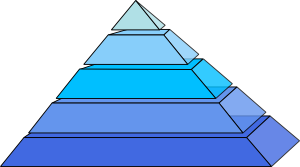
\includegraphics[width=1.1cm]{../Strukturfiler/FIGS/BluePyramid} & \begin{minipage}{\obsl}}{\end{minipage}\\ \end{tabular}\vspace{4mm}\newline}


% = Forudsætning = basis
\newenvironment{basis}{\begin{flushleft} \begin{itshape} }{\end{itshape} \end{flushleft}}


% = Opsummering =
\newenvironment{summary}{\clearpage\pagecolor{sumgul}\section{Opsummering}}{\newpage\pagecolor{white}}











% = Counter
\newcounter{opgavecount}[section]
\setcounter{opgavecount}{0}
\newcounter{spgcount}[opgavecount]
\setcounter{spgcount}{0}
\renewcommand{\thespgcount}{\alph{spgcount})}



% = EXERCISE = (DIVIDER)

\newcommand{\exercisebegin}[1][]{\bigskip\needspace{3\baselineskip}\refstepcounter{opgavecount}\titlegraphic{mingroen}\textcolor{mingroen}{\th{Opgave \theopgavecount \hspace*{1cm} #1}}\medskip\par}

% = QUIZEXERCISE = (DIVIDER)

\newcommand{\quizexercisebegin}[1][]{\bigskip\needspace{3\baselineskip}\refstepcounter{opgavecount}\titlegraphic{mingroen}\textcolor{mingroen}{\th{Quiz-Opgave \theopgavecount \hspace*{1cm} #1}}\medskip\par}

% = QUESTION =

\newenvironment{question}{\refstepcounter{spgcount}\begin{itemize}\item[\thespgcount]}{\end{itemize}\hspace*{\fill}}

% = VINK =

\newenvironment{vink}{\begin{tabular}{m{.9cm}<{\hspace*{2mm}}@{}|m{\obsl}@{}}\hspace*{-4pt}\raggedleft
\includegraphics[width=.9cm]{../Strukturfiler/FIGS/Think} & \begin{minipage}{\obsl}}{\end{minipage}\\ \end{tabular}\medskip\\}
	
% = FACIT =

\newenvironment{facit}{\begin{tabular}{m{.9cm}<{\hspace*{2mm}}@{}|m{\obsl}@{}}\hspace*{-4pt}\raggedleft
\includegraphics[width=.9cm]{../Strukturfiler/FIGS/Check} & \begin{minipage}{\obsl}}{\end{minipage}\\ \end{tabular}\medskip\\}








\newcommand{\afsnit}[1]{\bigskip\th{\titlegraphic{mingroen}\textcolor{mingroen}{#1}} \\ \rule[7pt]{.4\textwidth}{1pt} \vspace*{-2.5mm}\par}

% (DIVIDER):
\newcommand{\ugedagdatotitel}[4]{\pagebreak[4]\section{Semesteruge #1 -- #2 Dag \hspace*{1mm} (#3)} \vspace*{-4mm} \rule[5pt]{\textwidth}{1pt}\vspace*{-2.5mm} \begin{center}\large{\th{#4}}\end{center} \fancyhead[C]{\th{Semesteruge #1}}}

\newenvironment{skema}[1]{\definecolor{shadecolor}{rgb}{0.96,.98, 1.0} \setlength{\FrameSep}{6pt} \renewcommand{\FrameHeightAdjust}{10pt} \vspace*{-4pt}\begin{shaded} \begin{tabular}{#1}}{\end{tabular} \end{shaded} \vspace*{-7pt}}


% ========================

% MAKROER

%\newenvironment{matr}[1][]{\hspace*{-.8mm}\left[\hspace*{-1mm}\begin{array}{#1}}{\end{array}\hspace*{-1mm}\right]\hspace*{-.8mm}}
\newcommand{\bevisslut}{\begin{scriptsize} \begin{flushright} $ \blacksquare $ \end{flushright} \end{scriptsize}}

\newcommand{\tref}[2]{\hyperref[#1]{#2 \ref*{#1}}}
\newcommand{\thref}[2]{\hyperref[#1]{#2}}

\newcommand{\refA}[1]{\colorbox{yellow}{\ref{#1}}}
\newcommand{\hrefA}[2]{\colorbox{yellow}{\href{#1}{#2}}}
\newcommand{\trefA}[2]{\colorbox{yellow}{\hyperref[#1]{#2 \ref*{#1}}}}
\newcommand{\threfA}[2]{\colorbox{yellow}{\hyperref[#1]{#2}}}

\newenvironment{matr}[1]{\hspace*{-.8mm}\begin{bmatrix}\hspace*{-1mm}\begin{array}{#1}}{\end{array}\hspace*{-1mm}\end{bmatrix}\hspace*{-.8mm}}
\newcommand{\transp}{\hspace*{-.6mm}^{\top}}

\newcommand{\maengde}[2]{\left\lbrace \hspace*{-1mm} \begin{array}{c|c} #1 & #2 \end{array} \hspace*{-1mm} \right\rbrace}

\newenvironment{eqnalign}[1]{\setlength{\arraycolsep}{1.3pt}\begin{equation}\begin{array}{#1}}{\end{array}\end{equation}\par}
\newcommand{\eqnl}{\setlength{\arraycolsep}{1.3pt}}

\newcommand{\matind}[3]{{_\mathrm{#1}\mathbf{#2}_\mathrm{#3}}}
\newcommand{\vekind}[2]{{_\mathrm{#1}\mathbf{#2}}}
\newcommand{\jac}[2]{{\mathrm{Jacobi}_\mathbf{#1} (#2)}}
\newcommand{\diver}[2]{{\mathrm{div}\mathbf{#1} (#2)}}
\newcommand{\rot}[1]{{\mathbf{rot}\mathbf{(#1)}}}

\newcommand{\am}{\mathrm{am}}
\newcommand{\gm}{\mathrm{gm}}
\newcommand{\E}{\mathrm{E}}
\newcommand{\Span}{\mathrm{span}}
\newcommand{\mU}{\mathbf{U}}

\newcommand{\ms}{\medskip\\}
\newcommand{\bs}{\bigskip\\}

\newcommand{\mA}{\mathbf{A}}
\newcommand{\mB}{\mathbf{B}}
\newcommand{\mC}{\mathbf{C}}
\newcommand{\mD}{\mathbf{D}}
\newcommand{\mE}{\mathbf{E}}
\newcommand{\mF}{\mathbf{F}}
\newcommand{\mK}{\mathbf{K}}
\newcommand{\mI}{\mathbf{I}}
\newcommand{\mM}{\mathbf{M}}
\newcommand{\mN}{\mathbf{N}}
\newcommand{\mQ}{\mathbf{Q}}
\newcommand{\mT}{\mathbf{T}}
\newcommand{\mV}{\mathbf{V}}
\newcommand{\mW}{\mathbf{W}}
\newcommand{\mX}{\mathbf{X}}
\newcommand{\ma}{\mathbf{a}}
\newcommand{\mb}{\mathbf{b}}
\newcommand{\mc}{\mathbf{c}}
\newcommand{\md}{\mathbf{d}}
\newcommand{\me}{\mathbf{e}}
\newcommand{\mn}{\mathbf{n}}
\newcommand{\mr}{\mathbf{r}}
\newcommand{\mv}{\mathbf{v}}
\newcommand{\mw}{\mathbf{w}}
\newcommand{\mx}{\mathbf{x}}
\newcommand{\mxb}{\mathbf{x_{bet}}}
\newcommand{\my}{\mathbf{y}}
\newcommand{\mz}{\mathbf{z}}
\newcommand{\reel}{\mathbb{R}}
\newcommand{\mL}{\bm{\Lambda}} %Lambda-matrix
\newcommand{\mnul}{\bm{0}}
\newcommand{\trap}[1]{\mathrm{trap}(#1)}
\newcommand{\Det}{\operatorname{Det}}
\newcommand{\adj}{\operatorname{adj}}
\newcommand{\Ar}{\operatorname{Areal}}
\newcommand{\Vol}{\operatorname{Vol}}
\newcommand{\Rum}{\operatorname{Rum}}
\newcommand{\diag}{\operatorname{\bf{diag}}}
\newcommand{\bidiag}{\operatorname{\bf{bidiag}}}
\newcommand{\spanVec}[1]{\mathrm{span}\{#1\}}
\newcommand{\Div}{\operatorname{Div}}
\newcommand{\Rot}{\operatorname{\mathbf{Rot}}}

\newcommand{\Jac}{\operatorname{Jacobi}}
\newcommand{\Tan}{\operatorname{Tan}}
\newcommand{\Ort}{\operatorname{Ort}}
\newcommand{\Flux}{\operatorname{Flux}}
\newcommand{\Cmass}{\operatorname{Cm}}
\newcommand{\Imom}{\operatorname{Im}}
\newcommand{\Pmom}{\operatorname{Pm}}
\newcommand{\IS}{\operatorname{I}}
\newcommand{\IIS}{\operatorname{II}}
\newcommand{\IIIS}{\operatorname{III}}
\newcommand{\Le}{\operatorname{L}}
\newcommand{\app}{\operatorname{app}}
\newcommand{\M}{\operatorname{M}}
\newcommand{\re}{\mathrm{Re}}
\newcommand{\im}{\mathrm{Im}}

\newcommand{\compl}{\mathbb{C}} %de komplekse tal
\newcommand{\e}{\mathrm{e}} %eksponentialfunktionen. lodret 'e', og altså ikke kursiv ligesom andre bogstaver.





% Medialink: SCREEN: (QRcode) + thumbnail image + link på kodenummer (til qr.dtu.dk)
\newcommand{\onlinemedia}[3]{
	\begin{wrapfigure}{r}{3.2cm} 
		\vspace{-30pt} 
		\vspace{#1pt} 
		\begin{flushright} 
			\includegraphics[width=3cm]{qr/#2.png} 
			\tiny 
			\href{http://qr.dtu.dk/#2}{#2: #3}
			\normalsize  
		\end{flushright} 
		\vspace{-10pt} 
	\end{wrapfigure}
}
\newcommand{\onlinemediathumb}[3]{
	\begin{wrapfigure}{r}{3.2cm} 
		\vspace{-30pt} 
		\vspace{#1pt} 
		\begin{flushright} 
			\includegraphics[width=3cm]{qr/#2.png} 
			\includegraphics[width=3cm]{qr/#2_thumb.png} 
			\tiny 
			\href{http://qr.dtu.dk/#2}{#2: #3}
			\normalsize  
		\end{flushright} 
		\vspace{-10pt} 
	\end{wrapfigure}
}



% Index:
\usepackage{makeidx}
\makeindex
\newcommand\ind[2]{\index{#1}\textbf{\textit{\textcolor{black}{#2}}}}

% ###SERVER_EXCLUDE_BEGIN###
\externaldocument[NUID17-]{../../enoten/TN01-Talrum/Talrum}
\externaldocument[NUID1-]{../../enoten/TN02-Ligningssystemer/TNdriver}
\externaldocument[NUID2-]{../../enoten/TN03-Matricer_og_Matrixalgebra/Matricer_og_matrixalgebra}
\externaldocument[NUID3-]{../../enoten/TN04-Kvadratiske_matricer/TNdriver}
\externaldocument[NUID11-]{../../enoten/TN05-Determinanter/Determinanter}
\externaldocument[NUID12-]{../../enoten/TN06-GeometriskeVektorer/GeometriskeVektorer}
\externaldocument[NUID18-]{../../enoten/TN07-Vektorrum/VektorRum}
\externaldocument[NUID21-]{../../enoten/TN08-LinAfbildninger/LinAfbildninger}
\externaldocument[NUID23-]{../../enoten/TN09-Egenvaerdier_og_egenvektorer/TNdriver}
\externaldocument[NUID24-]{../../enoten/TN10-Diagonalisering_med_egenvektorer/TNdriver}
\externaldocument[NUID10-]{../../enoten/TN11-1.ordens_differentialligninger/TNdriver}
\externaldocument[NUID13-]{../../enoten/TN12-1.ordens_differentialligningssystemer/TNdriver}
\externaldocument[NUID14-]{../../enoten/TN13-2.ordens_differentialligninger/TNdriver}
\externaldocument[NUID27-]{../../enoten/TN14-Elemenataere_funktioner/Elementaere_Funktioner}
\externaldocument[NUID28-]{../../enoten/TN15-Funktioner2Variable/Funktioner_To_Variable}
\externaldocument[NUID29-]{../../enoten/TN16-Gradienter_og_Tangentplaner/Gradienter_og_Tangentplaner}
\externaldocument[NUID32-]{../../enoten/TN17-Taylor_formler/Taylor_Formler}
\externaldocument[NUID33-]{../../enoten/TN18-Taylor_2Var/Taylor_2Var}
\externaldocument[NUID34-]{../../enoten/TN19-SymMat/SymmetriskeMatricer}
\externaldocument[NUID35-]{../../enoten/TN20-KegleSnit/Keglesnit}
\externaldocument[NUID36-]{../../enoten/TN21-Riemann_Integral/Riemann_01}
\externaldocument[NUID37-]{../../enoten/TN22-Plan_Int/Plan_Int_01}
\externaldocument[NUID39-]{../../enoten/TN23-Flade_Int/Flade_Rum_Int_01}
\externaldocument[NUID40-]{../../enoten/TN24-Vektorfelter/Vektorfelter_01}
\externaldocument[NUID41-]{../../enoten/TN25-Flux/Flux_02}
\externaldocument[NUID42-]{../../enoten/TN26-Gauss/Gauss_01}
\externaldocument[NUID128-]{../../enoten/TN27-Stokes/Stokes_01}
\externaldocument[NUID43-]{../../enoten/TN29-KomplekseTal/KomplekseTal}

\externaldocument[NUID6-]{../../E-math-opgaver/Opgaver/opgU123}
\externaldocument[NUID19-]{../../E-math-opgaver/Opgaver/opgU45}
\externaldocument[NUID20-]{../../E-math-opgaver/Opgaver/opgU678}
\externaldocument[NUID25-]{../../E-math-opgaver/Opgaver/opgU910SD}
\externaldocument[NUID31-]{../../E-math-opgaver/OpgaverF11-U123/opgF123}
% \externaldocument[NUID9-]{../../E-math-opgaver/Opgaver/Dagsordner E10}
% ###SERVER_EXCLUDE_END###


% Begin document and set alternative chapter title:
\begin{document}
\renewcommand{\chaptername}{eNote}

\setcounter{chapter}{14} %SÆT DETTE TAL TIL 1 MINDRE END DET AKTUELLE TRANSFERNOTE-NUMMER!!

%%%%%%%%%%%%%%%%%%%%%%%%%%%%%%%%%%%%%%%%%%%%%
%%%%%%%%%%%%%%%%%%%%%%%%%%%%%%%%%%%%%%%%%%%%%
%%% HERFRA SKAL DU SKRIVE ELLER INDSÆTTE %%%%
%%% DEN FIL DU ØNSKER %%%%%%%%%%%%%%%%%%%%%%%
%%%%%%%%%%%%%%%%%%%%%%%%%%%%%%%%%%%%%%%%%%%%%
%%%%%%%%%%%%%%%%%%%%%%%%%%%%%%%%%%%%%%%%%%%%%


% REF: TransferNote \ref{TN4-tn4} \nameref{TN4-tn4}
%
% \tref{NUID14-thm.koma}{sætning}
%
% \tref{NUID14-tn13}{eNote}


\chapter{Funktioner af to variable} \label{tn15}


\begin{basis}
I denne og i de efterfølgende eNoter vil vi udvide funktionsbegrebet til at omfatte reelle funktioner af flere variable;  vi starter udvidelsen med $2$ variable, så vi vil i denne eNote definere værdimængder, kontinuitet, og differentiabilitet af funktioner $f(x,y)$ af to variable, her $x$ og $y$. Ligesom for funktioner af \'{e}n variabel vil vi bruge epsilon-funktions-begrebet (nu ligeledes af to variable) til formålet.
\end{basis}


%%%%%%%%%%%%%%%%%%%%%%%%%%%%%%%%%%%%%%%%%%%%%%%%%%%%%%%%%%%%%
%%%%%%%%%%%%%%%%%%%%%%%%%%%%%%%%%%%%%%%%%%%%%%%%%%%%%%%%%%%%%
%%%%%%%%%%%%%%%%%%%%%%%%%%%%%%%%%%%%%%%%%%%%%%%%%%%%%%%%%%%%%



\section{Definitionsmængder} \label{secDefVal}
Ved beskrivelsen af en reel funktion $f(x,y)$ af to variable anføres dels de punkter $(x, y)$, i $(x,y)$-planen hvor funktionen er defineret, og dels de
værdier, som kan fås ved at benytte funktionen på defintionsmængden. \ind{definitionsmængde}{Definitionsmængden} kalder vi $\mathcal{D}m(f)$ og \ind{værdimængde}{værdi\-mængden} kalder vi $\mathcal{V}m(f)$. Det er især definitionsmængderne vi vil fokusere på her. \\

Som noget nyt i forhold til funktioner af \'{e}n variabel er definitionsmængderne i planen generelt ikke så simple som intervallerne på den reelle talakse.

\begin{example}[Definitionsmængde for en funktion af to variable]
Lad os se på en funktion $f(x,y)$ af to variable:
\begin{equation}
f(x,y) = \ln(\sqrt{5 - x^{2} - y^{2}}) \quad .
\end{equation}
For hvilke punkter $(x,y)$ i $\mathbb{R}^{2}$ er denne funktion defineret? Vi
har f.eks. at $f(0,0) = \ln(\sqrt{5})$, $f(2,0) = f(0,2) = 0$, $f(1,0) = f(0,1) = \ln(2)$, og faktisk er $f(\cos(t), \sin(t)) = \ln(2)$ for alle $t$, men $f(3, 7)$ er ikke defineret for denne funktion. Ved inspektion af funktionen ses det, at definitionsmængden for $f(x,y)$ består præcis af de punkter, der ligger helt inde i den cirkelskive, der har centrum i $(0,0)$ og radius $\sqrt{5}$:
\begin{equation}
\mathcal{D}m(f) = \maengde{(x,y) \in \mathbb{R}^{2}}{x^{2} + y^{2} < 5} \quad.
\end{equation}
Læg mærke til, at cirkel-randen af cirkelskiven ikke er med i definitionsmængden.
\end{example}

Vi vil nu  indføre nogle vigtige begreber til beskrivelse af definitionsmængder og iøvrigt generelt til beskrivelse af vilkårlige delmængder af $(x,y)$-planen som kan være gode at benytte sig af, når man f.eks. skal tegne eller skitsere mængderne:

\subsection{Åbne og afsluttede mængder i planen}

\begin{definition}[Åbne mængder i planen] \label{defAAbenMgd}
En delmængde eller et område $M$  i planen kaldes \ind{åben mængde}{en åben mængde} hvis
ethvert punkt $(x_{0}, y_{0})$ i mængden er centrum for en eller anden (gerne meget lille) cirkelskive, som
selv er helt indeholdt i $M$.
\end{definition}

\begin{example}[En cirkelskive]
Mængden $\mathcal{D}m = \maengde{(x,y) \in \mathbb{R}^{2}}{x^{2} + y^{2} < 5}$ er en åben mængde. Men mængden
 $\maengde{(x,y) \in \mathbb{R}^{2}}{x^{2} + y^{2} \leq 5}$ er \emph{ikke} en åben mængde.
\end{example}

\begin{definition}[Randen af en mængde i planen, indre og ydre] \label{defAAbenMgd}
\ind{randen af et område}{Randen af et område} $M$  i planen består af de punkter $(x_{0}, y_{0})$ \emph{i planen} som har følgende egenskab:
Enhver cirkelskive med centrum i $(x_{0}, y_{0})$ indeholder både punkter som tilhører $M$ og punkter som ikke tilhører $M$.
Bemærk, randpunkterne for $M$ ikke selv behøver at være med i mængden $M$. Mængden af randpunkter for $M$ betegnes med $\partial M$.\\

\ind{indre af et område}{Det indre af et område} $M$ er alle de punkter i $M$, som ikke ligger på randen af $M$. Det indre af $M$ betegnes med $\mathring{M}$.\\

\ind{ydre af et område}{Det ydre af et område} $M$ i planen er alle de punkter i planen som ikke tilhører hverken $M$ eller  $\partial M$.
\end{definition}

\begin{example}[Randen af en åben cirkelskive]
Mængden $\mathcal{D}m = \maengde{(x,y) \in \mathbb{R}^{2} }{x^{2} + y^{2} < 5}$ har randen:
\begin{equation}
\partial \mathcal{D}m = \maengde{(x,y) \in \mathbb{R}^{2} }{x^{2} + y^{2} =  5} \quad .
\end{equation}
\end{example}

\begin{definition}[Afslutningen af en mængde i planen]
Hvis en mængde $M$ tilføjes sine randpunkter $\partial M$ fås  \ind{afslutningen af en mængde}{afslutningen} af mængden som  betegnes med:
\begin{equation}
\bar{M} = M \, \cup \, \partial M \quad.
\end{equation}
Hvis randpunkterne allerede er med i mængden $M$ fås ikke derved nogen udvidelse af $M$. Mængden $M$ kaldes \ind{afsluttet mængde}{afsluttet} hvis $\bar{M} = M$.
\end{definition}

\begin{example}[Figurativt om åbne og afsluttede mængder]
Mængden $A$ i figur \ref{figDefMgd} er hverken åben eller afsluttet (der er nogle punkter på randen, som selv er med i mængden og der er andre punkter på randen som ikke er med i mængden. Tegne-forskriften er følgende: Punkter, der er med i mængden er grønne eller ligger på en fuldt optrukket stykke af randen; punkter, der ikke er med i mængden er ikke farvede eller (hvis de er en del af randen) markerede med røde cirkler. Mængden $B$ i figur  \ref{figDefMgd} er en åben mængde. Mængden $C$ i figur  \ref{figDefMgd} er en afsluttet mængde.
\end{example}



\begin{figure}[h]
\centerline{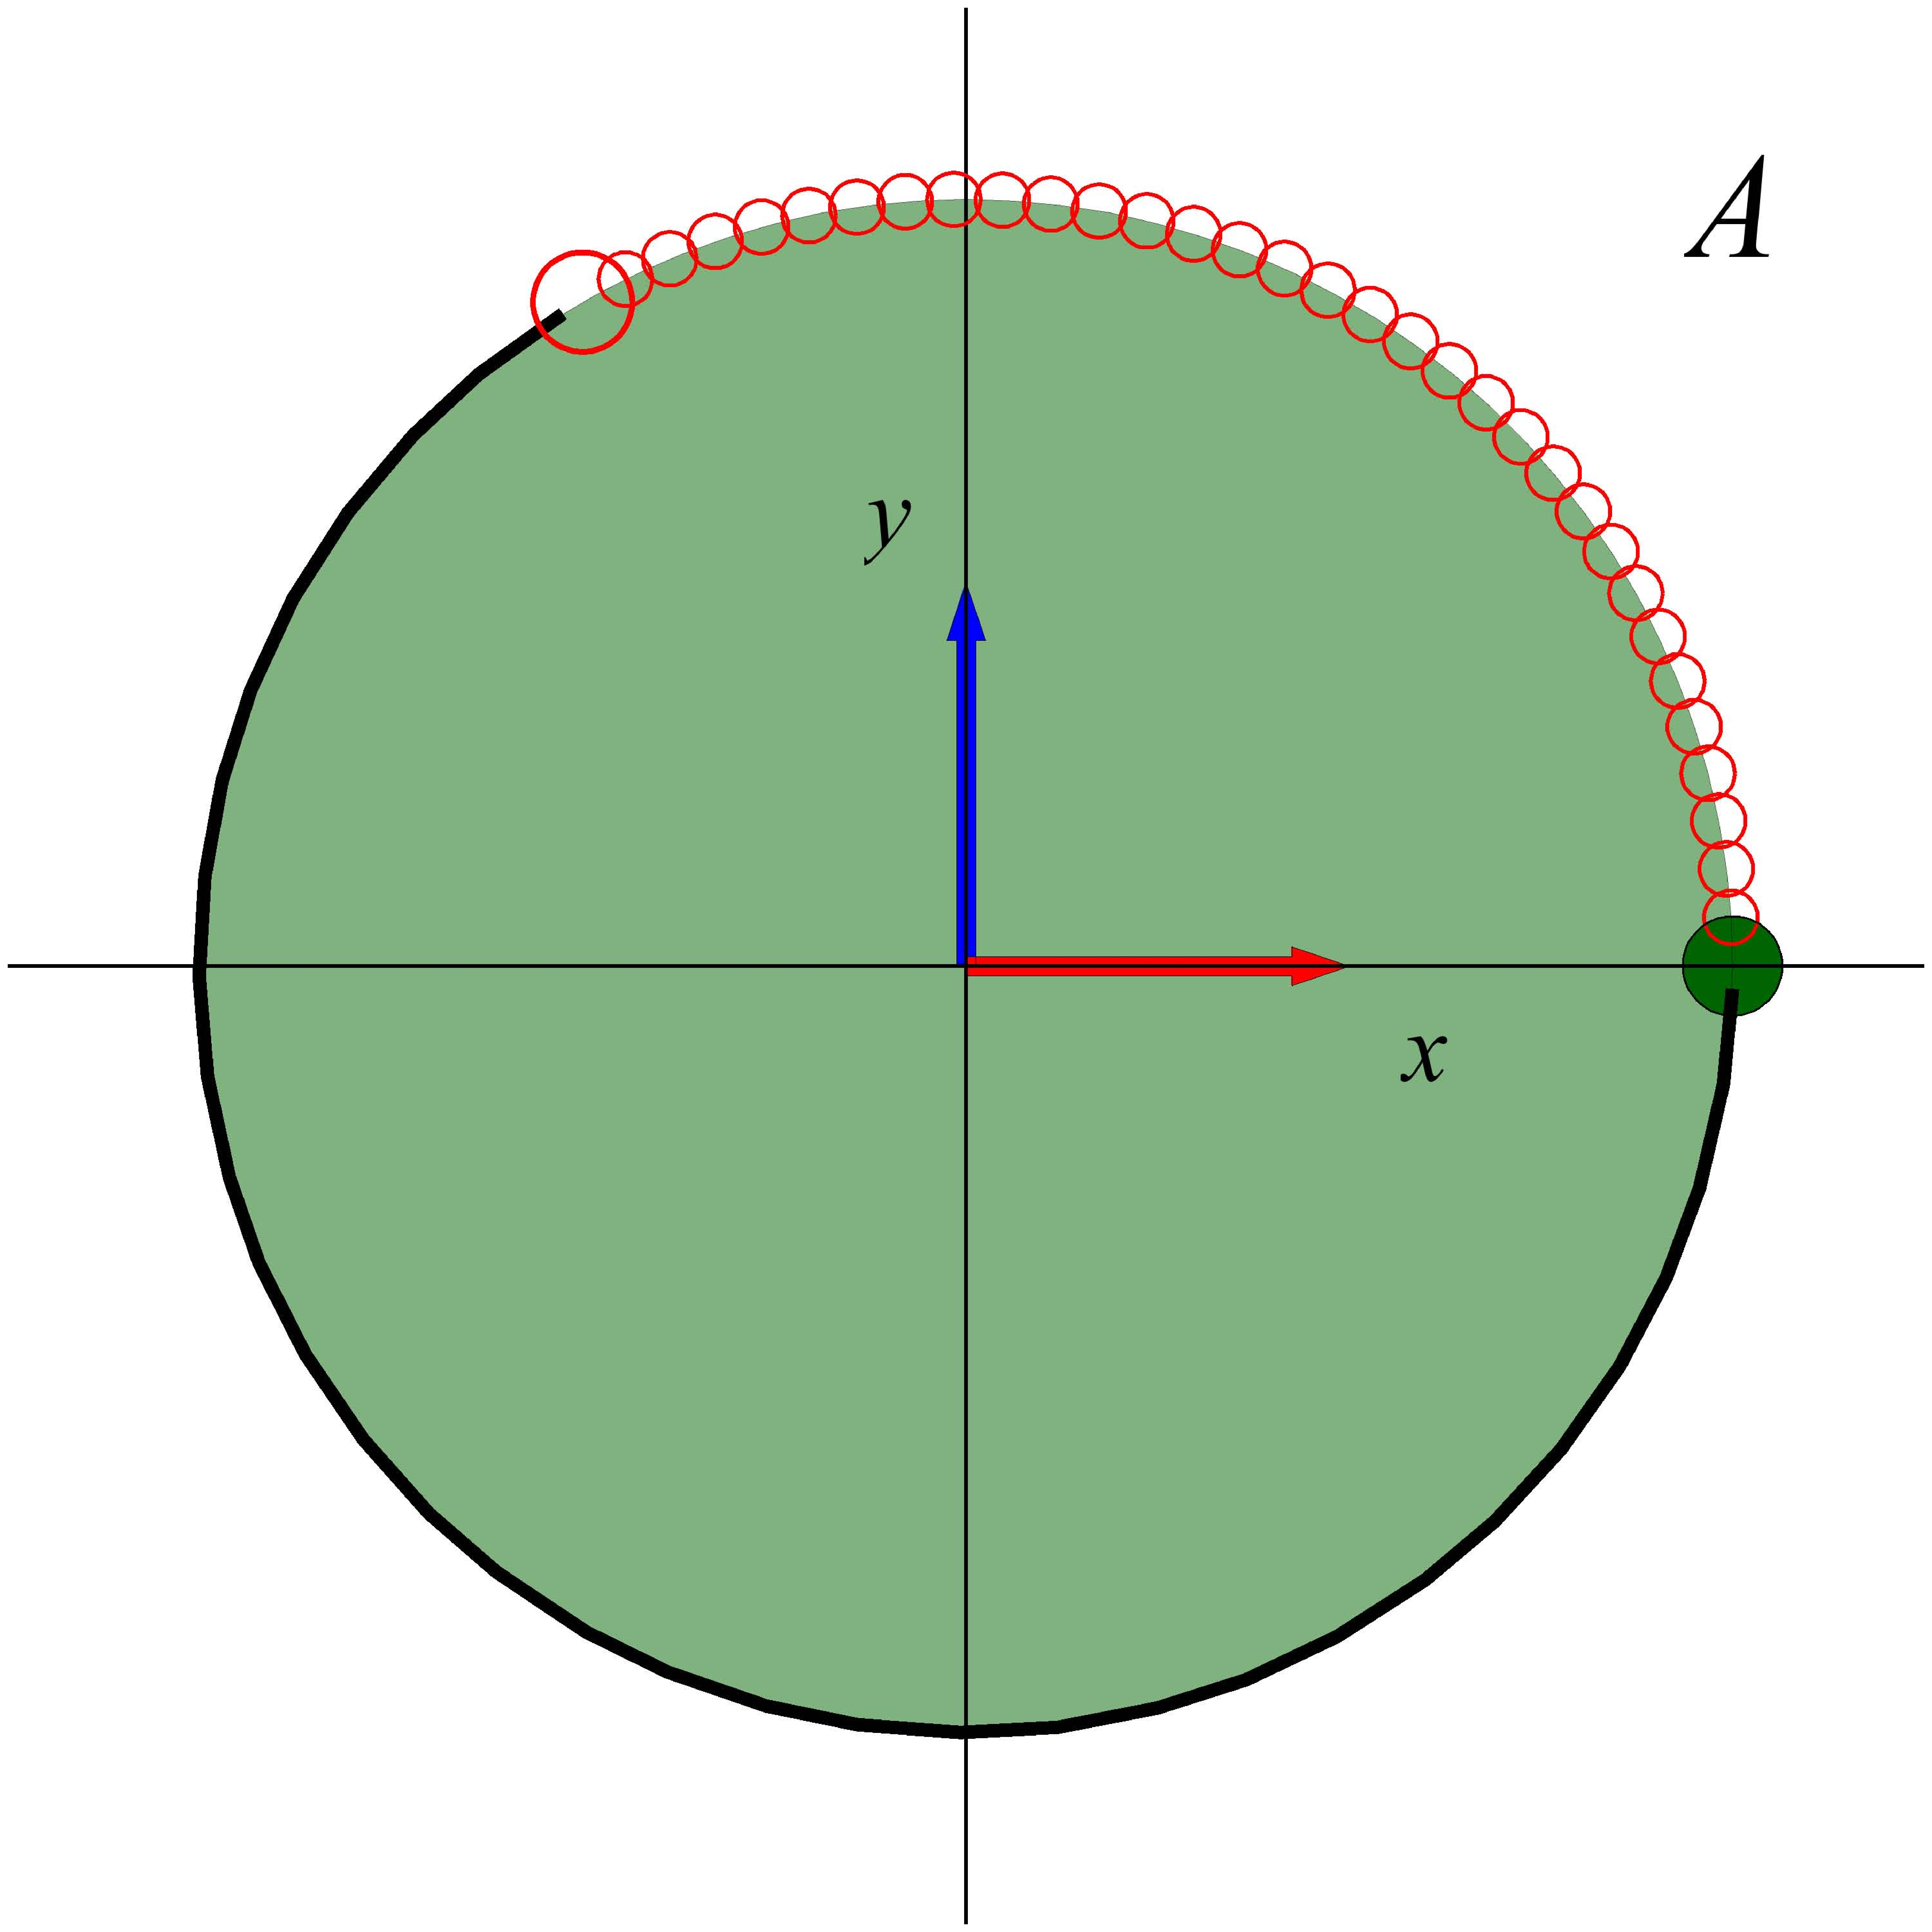
\includegraphics[height=55mm]{plotDefmgd1.pdf}\quad 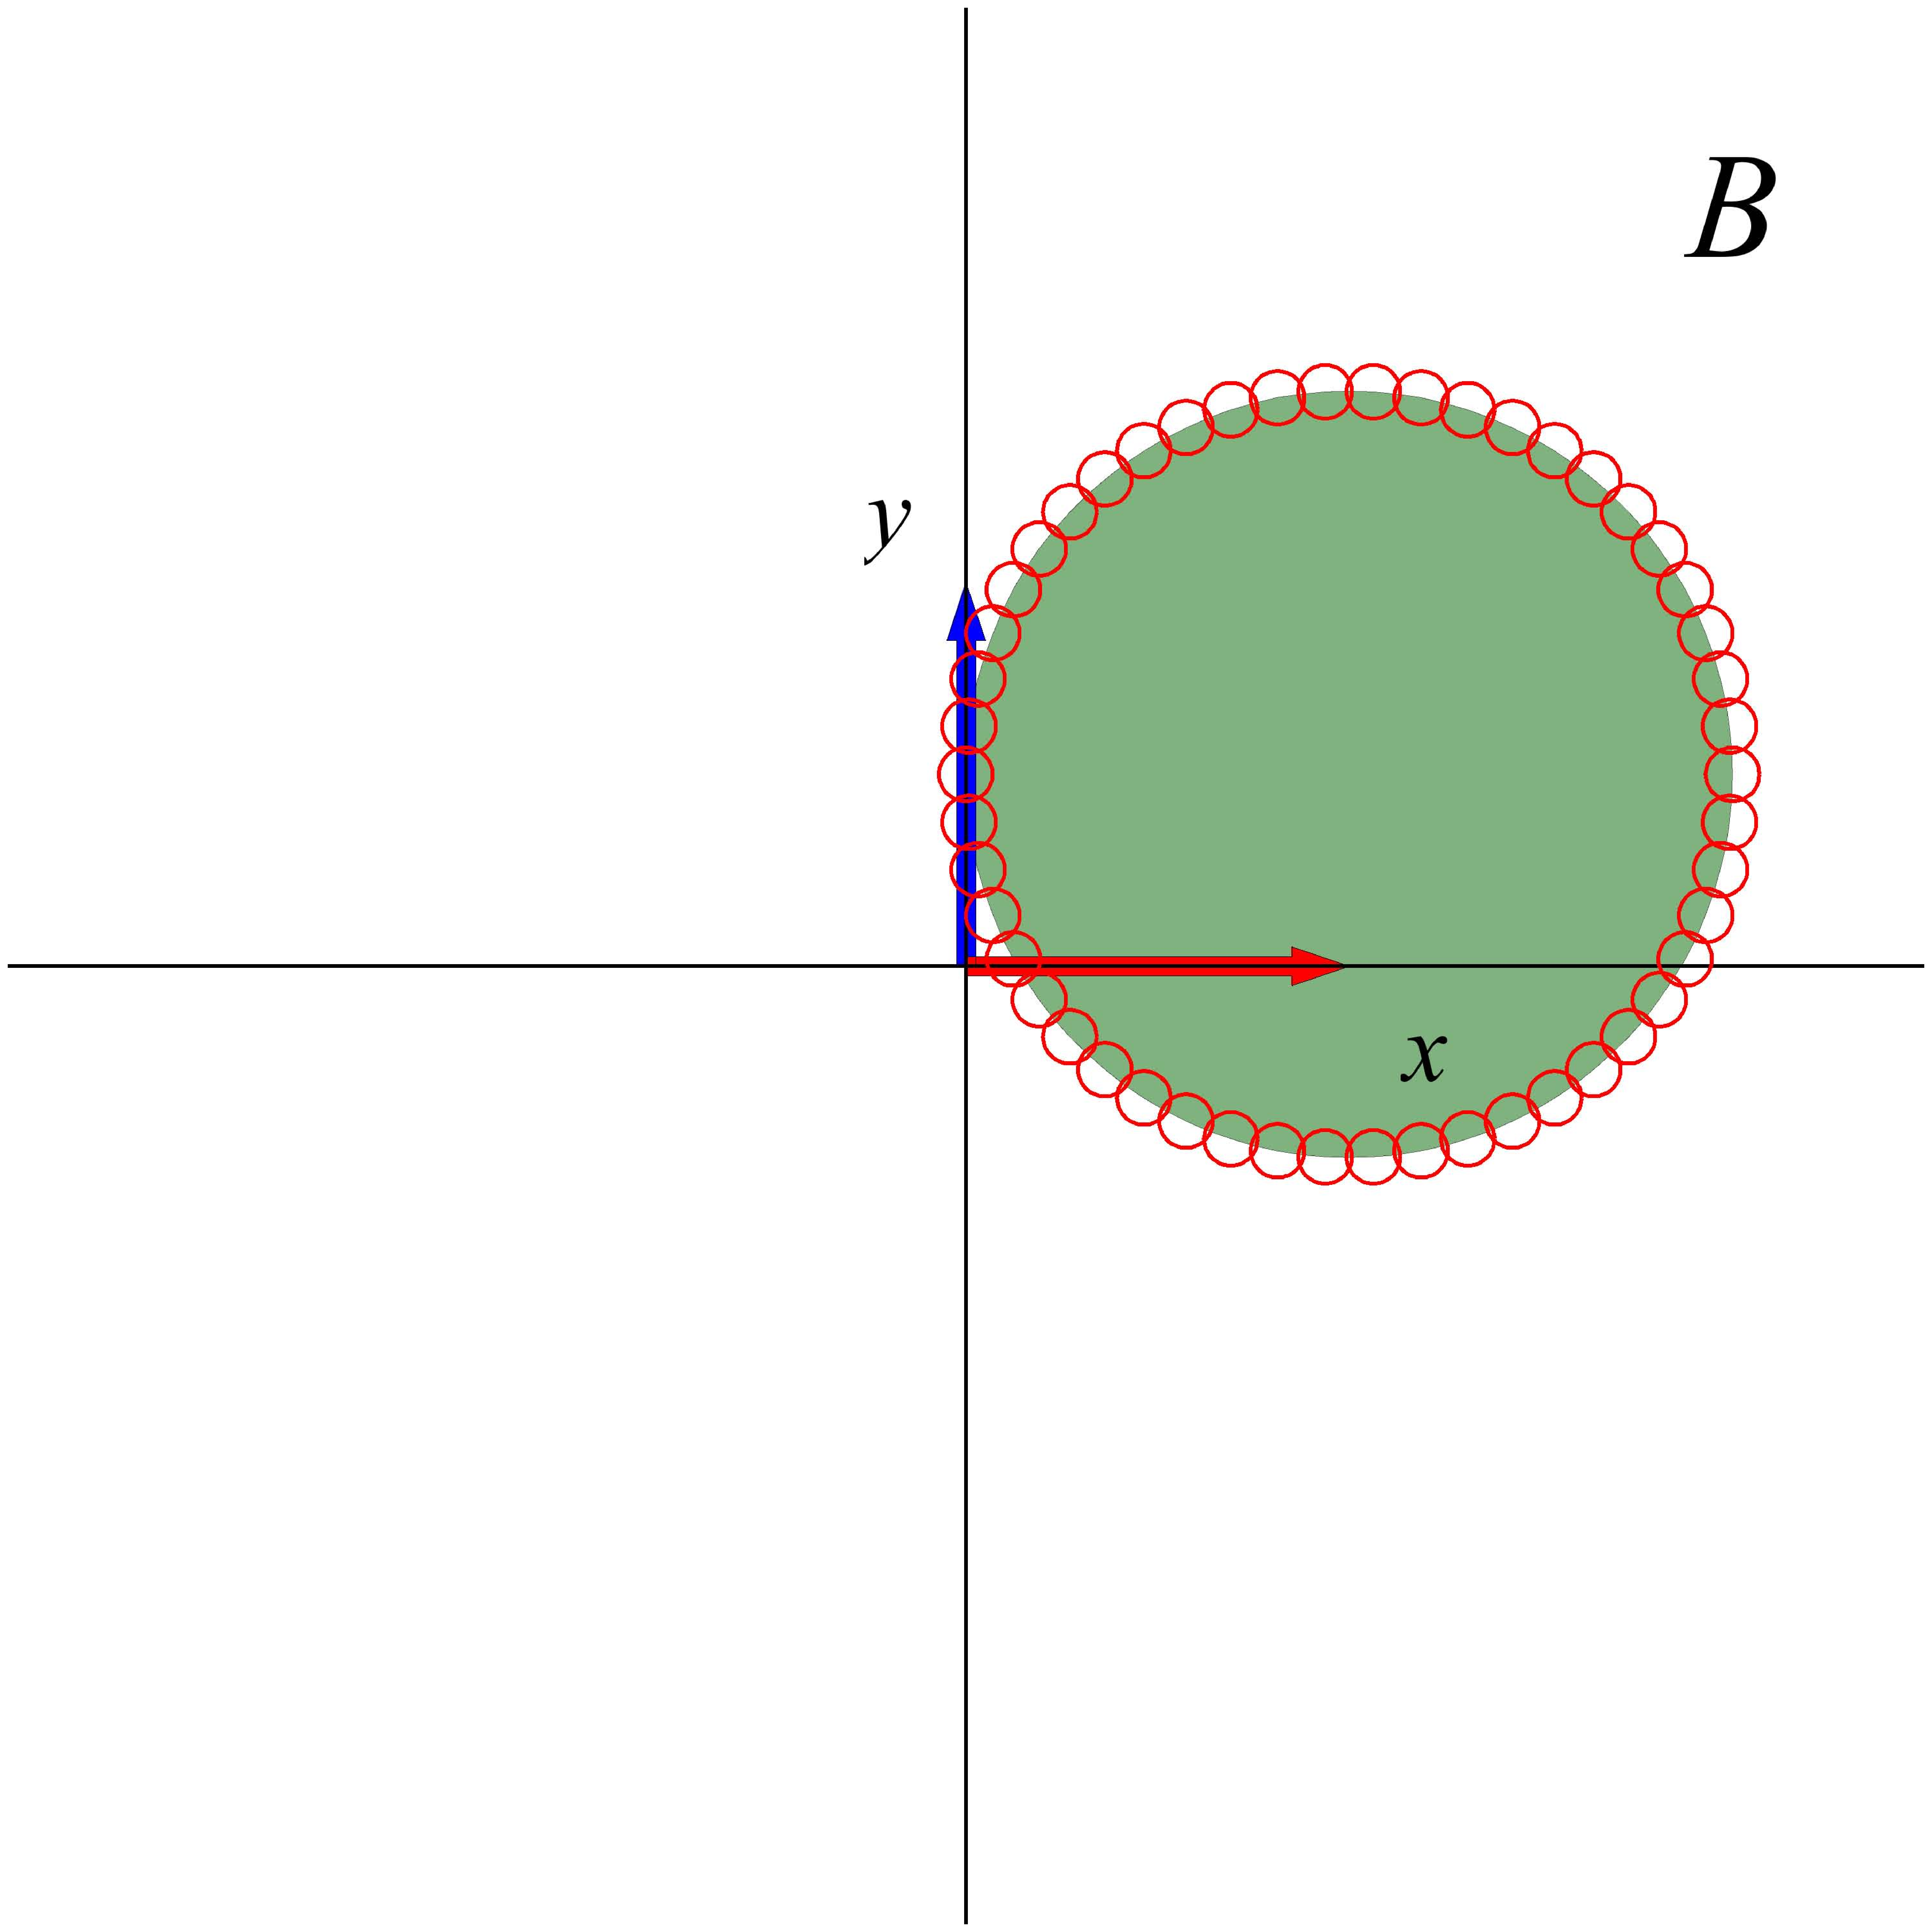
\includegraphics[height=55mm]{plotDefmgd2.pdf}\quad 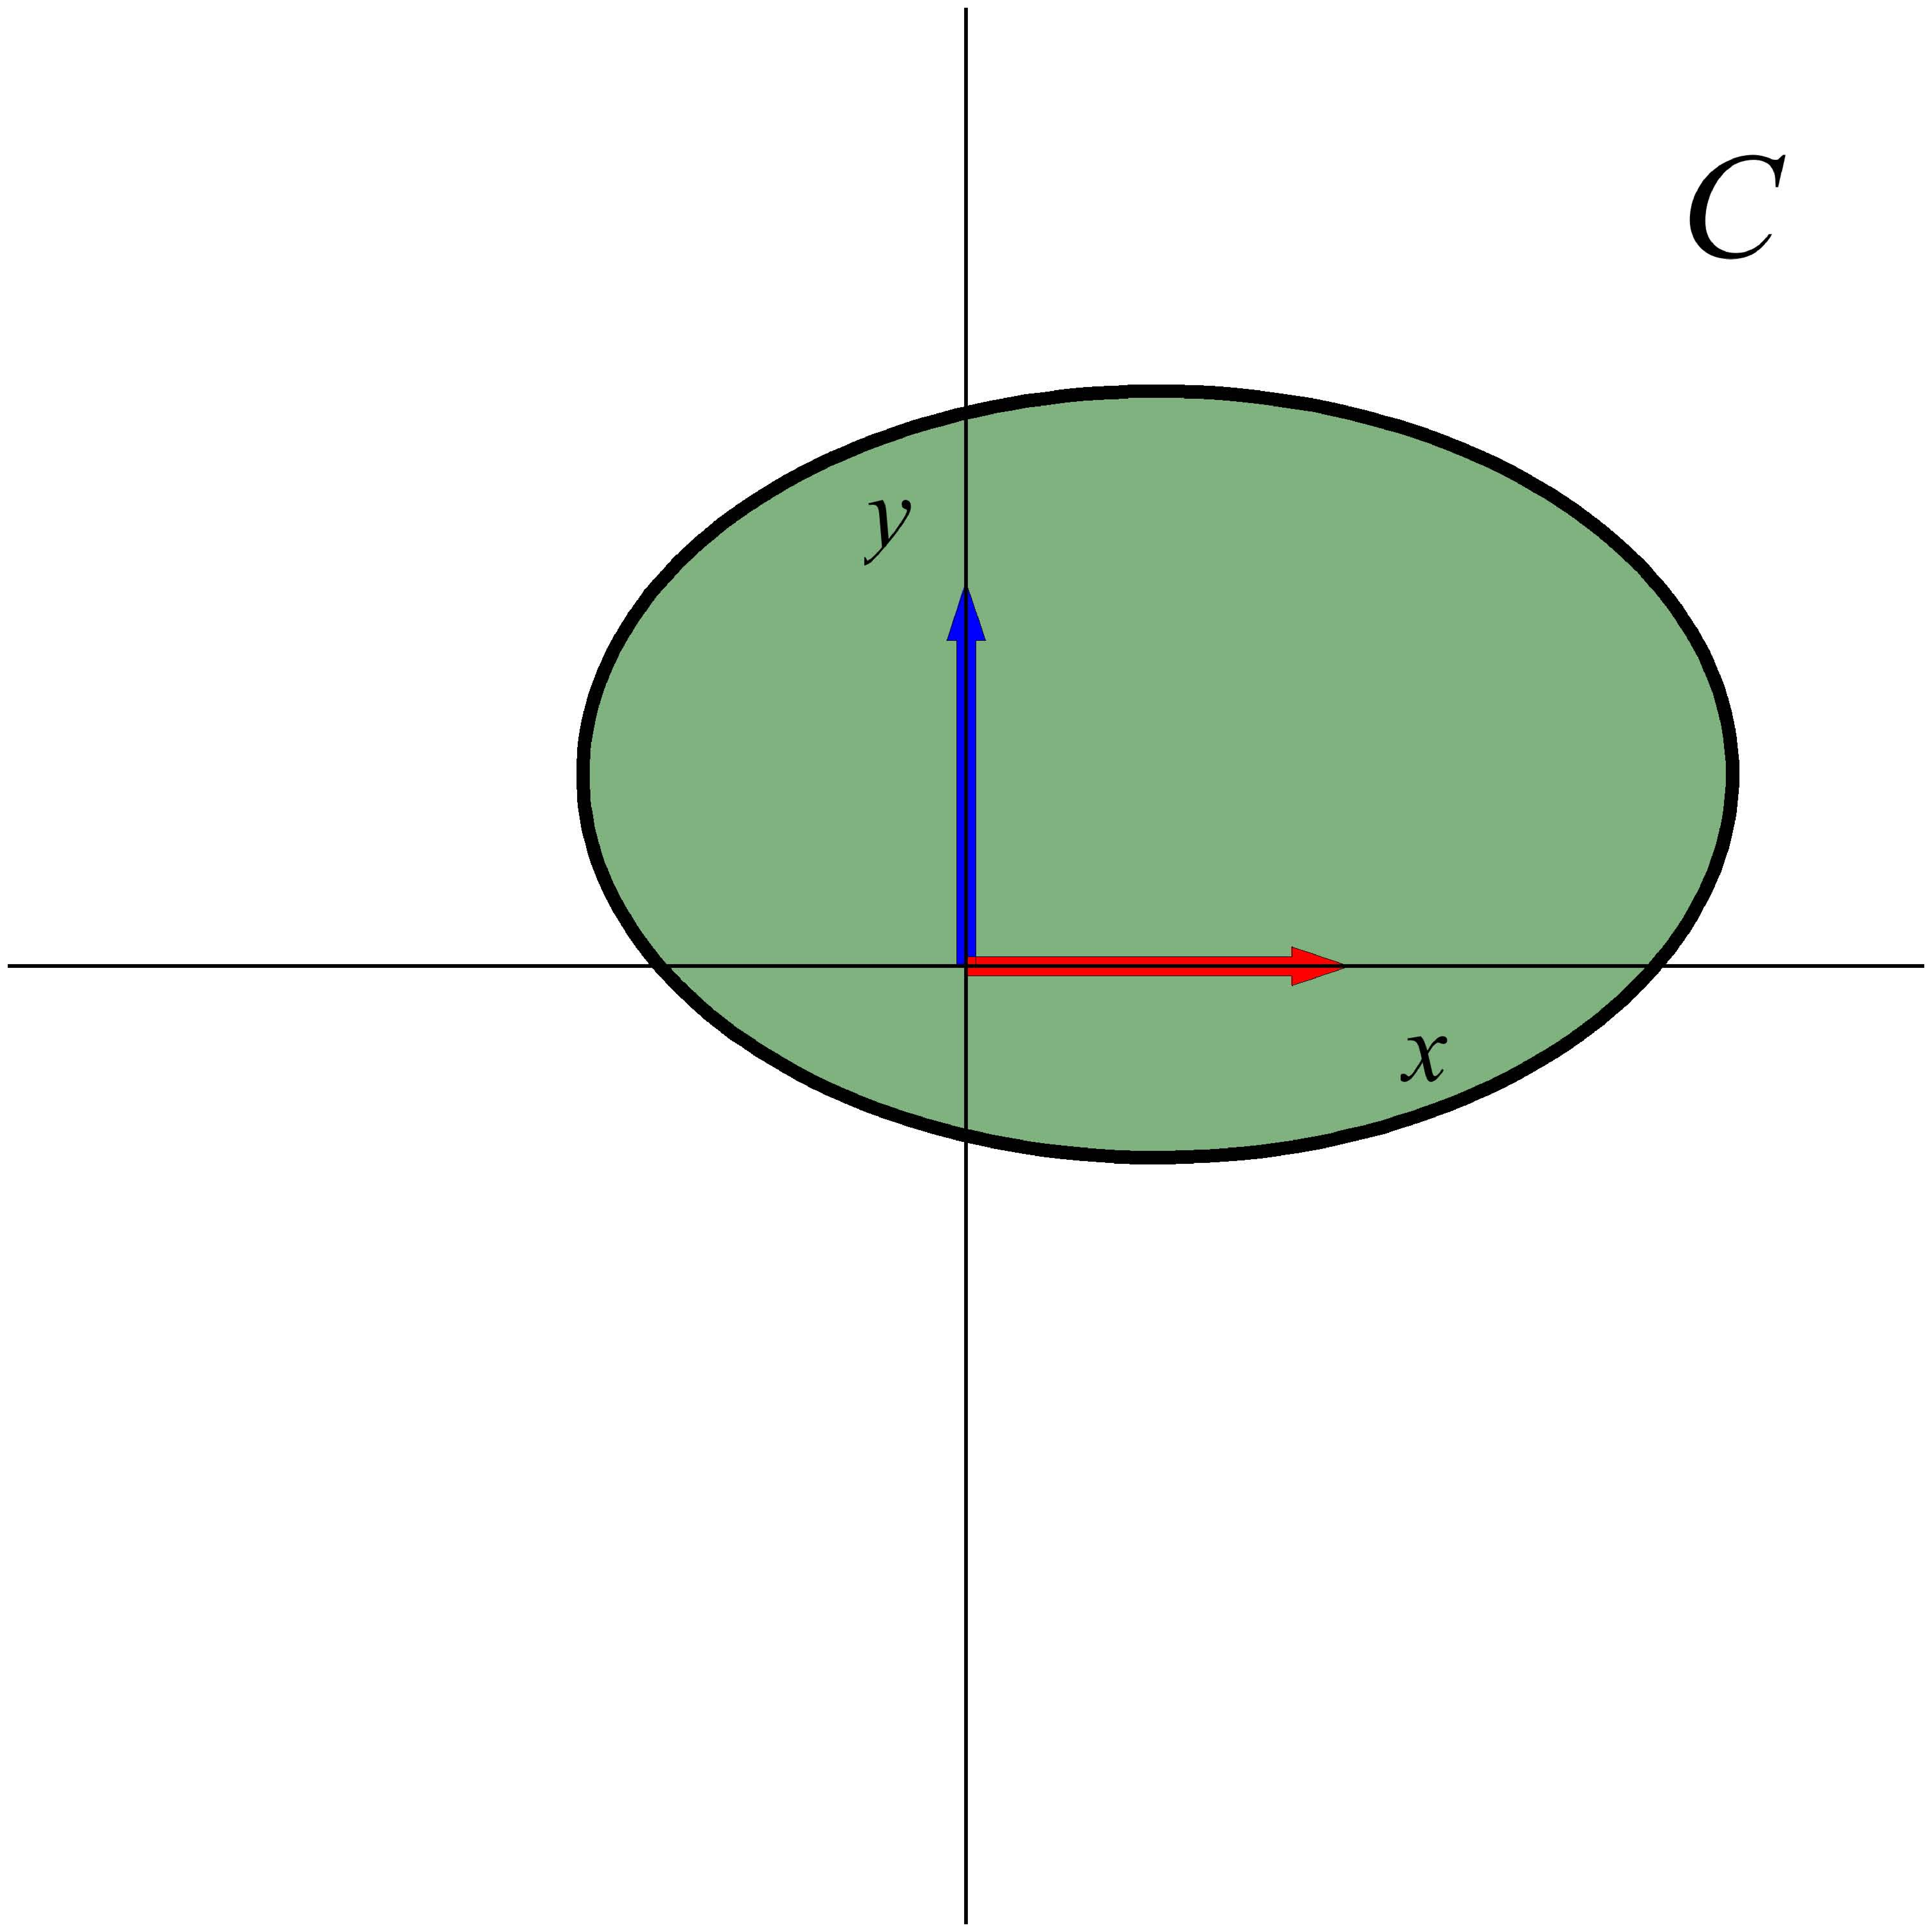
\includegraphics[height=55mm]{plotDefmgd3.pdf}}
\begin{center}
\caption{Områder i planen. Mængden $A$ er hverken åben eller afsluttet, $B$ er en åben mængde, og $C$ er en afsluttet mængde.} \label{figDefMgd}
\end{center}
\end{figure}


\begin{figure}[h]
\centerline{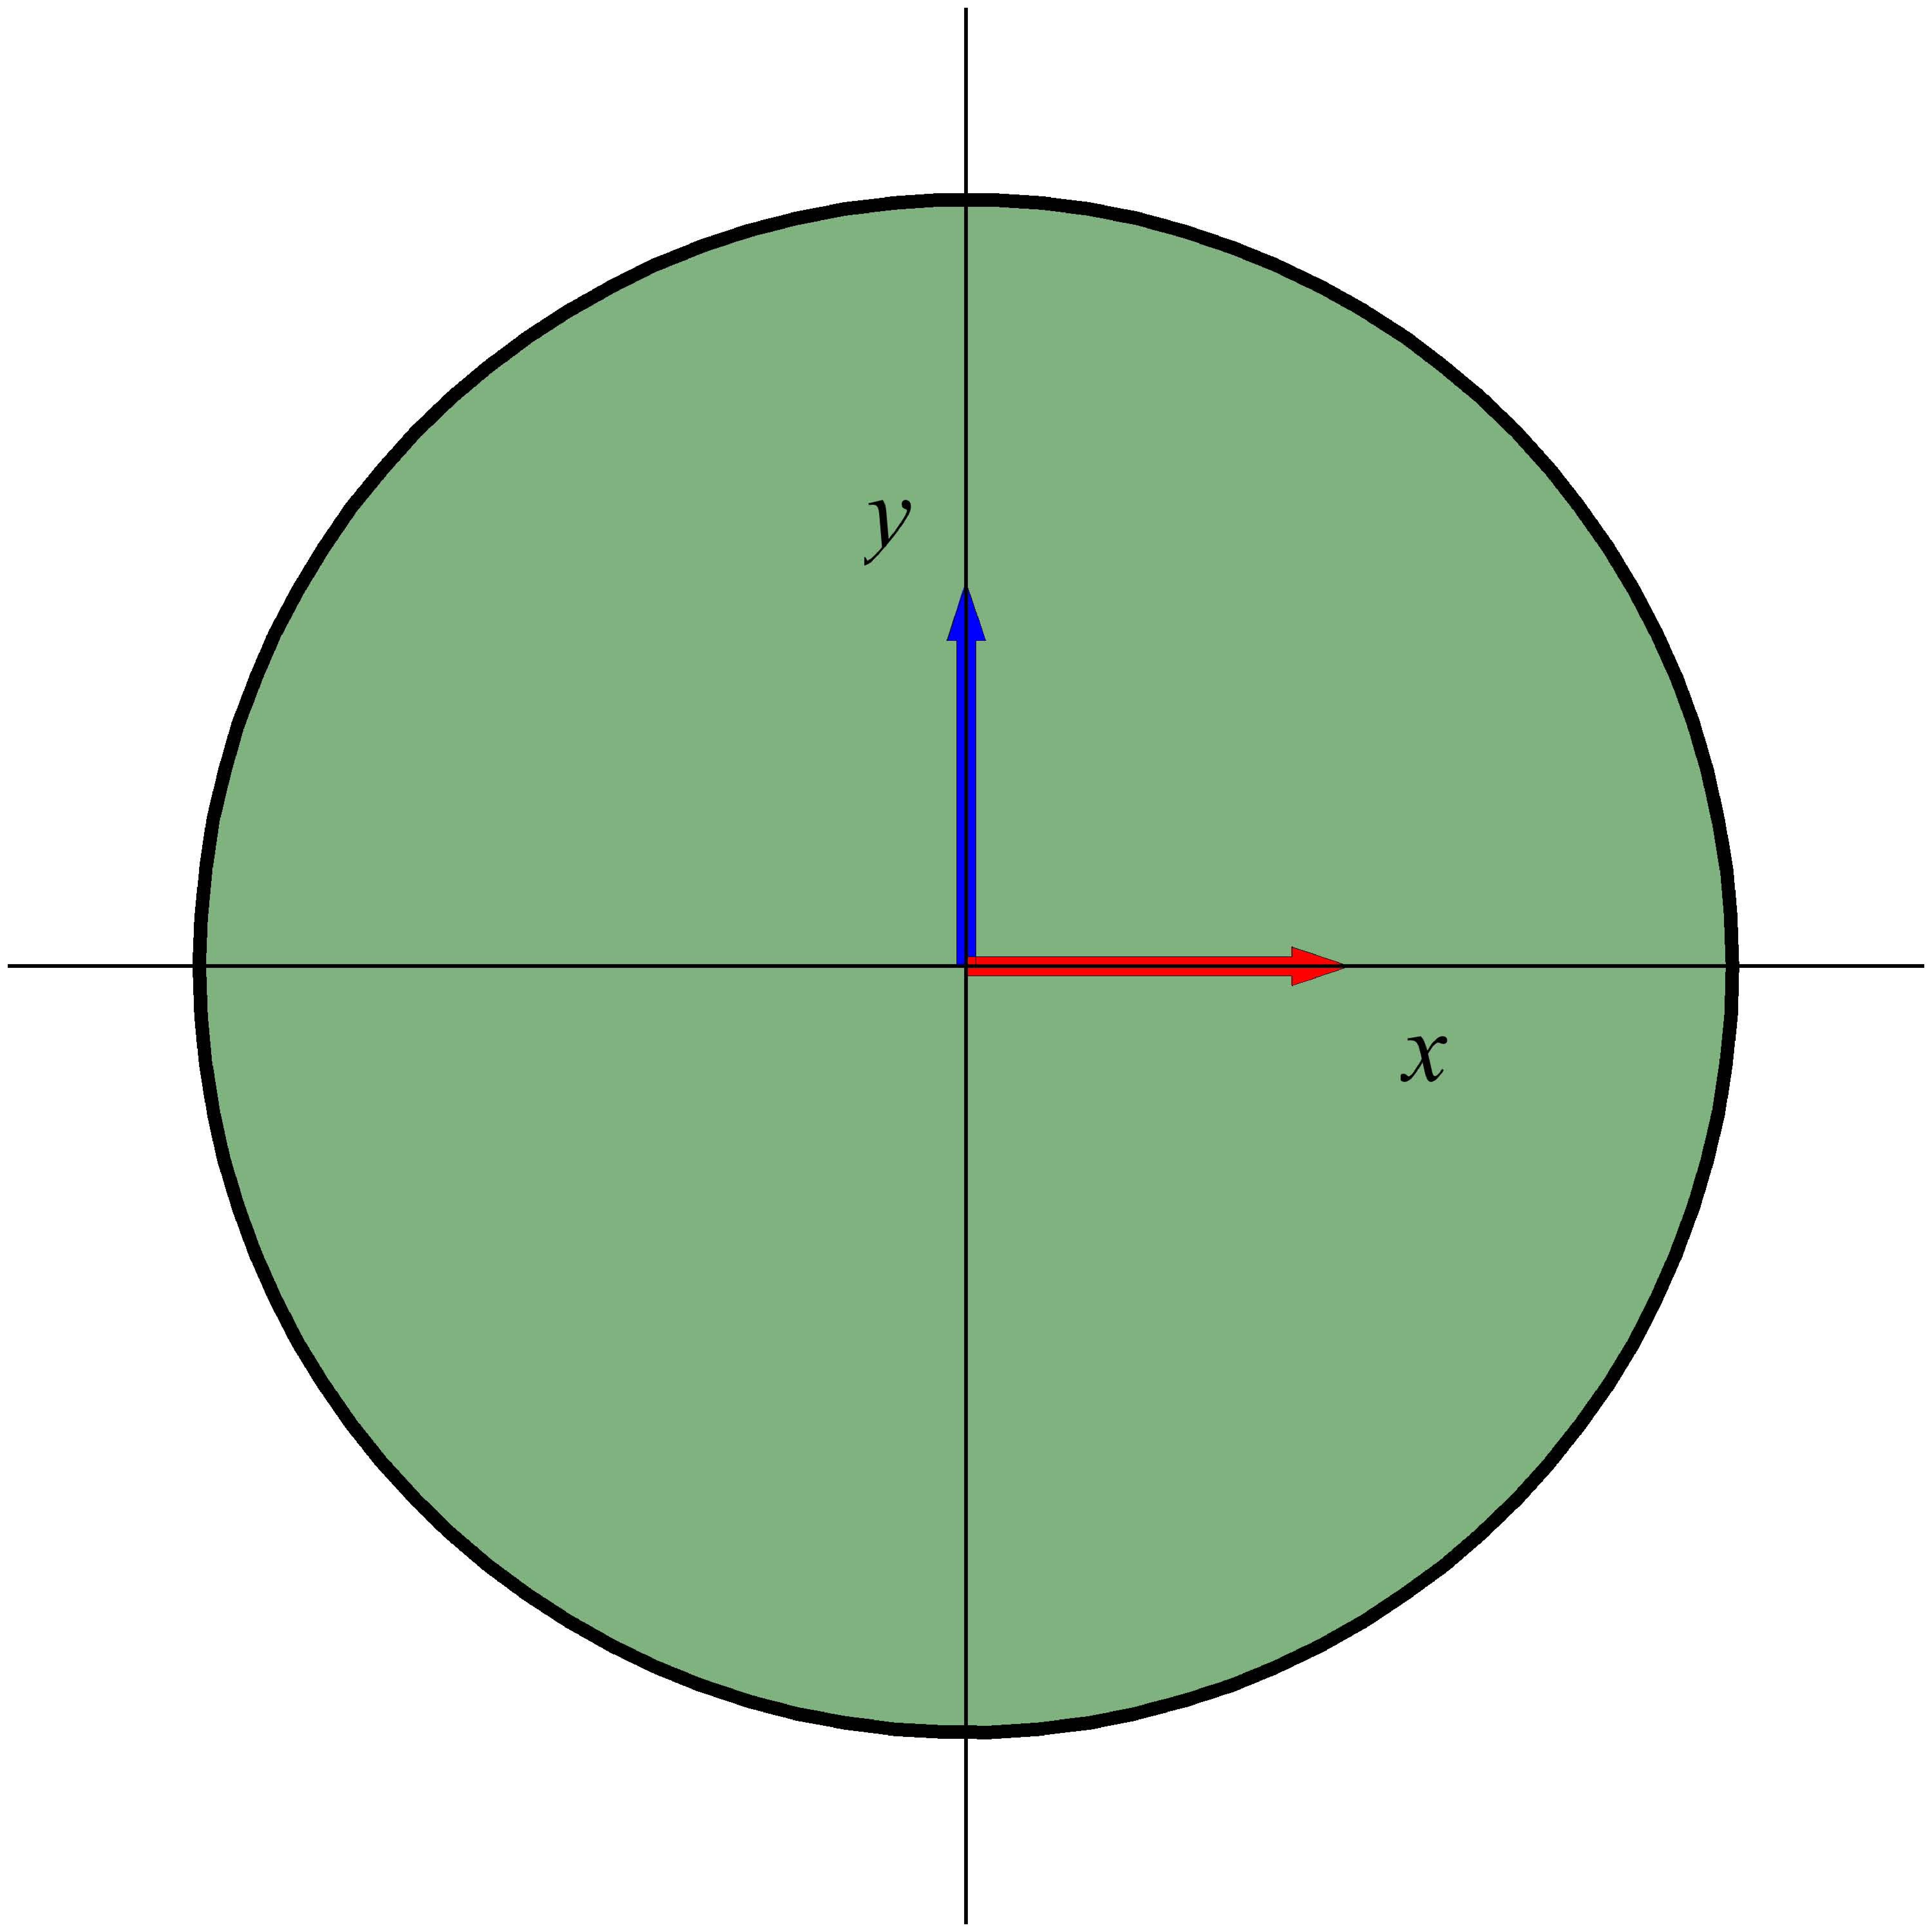
\includegraphics[height=55mm]{plotAfs1.pdf}\quad 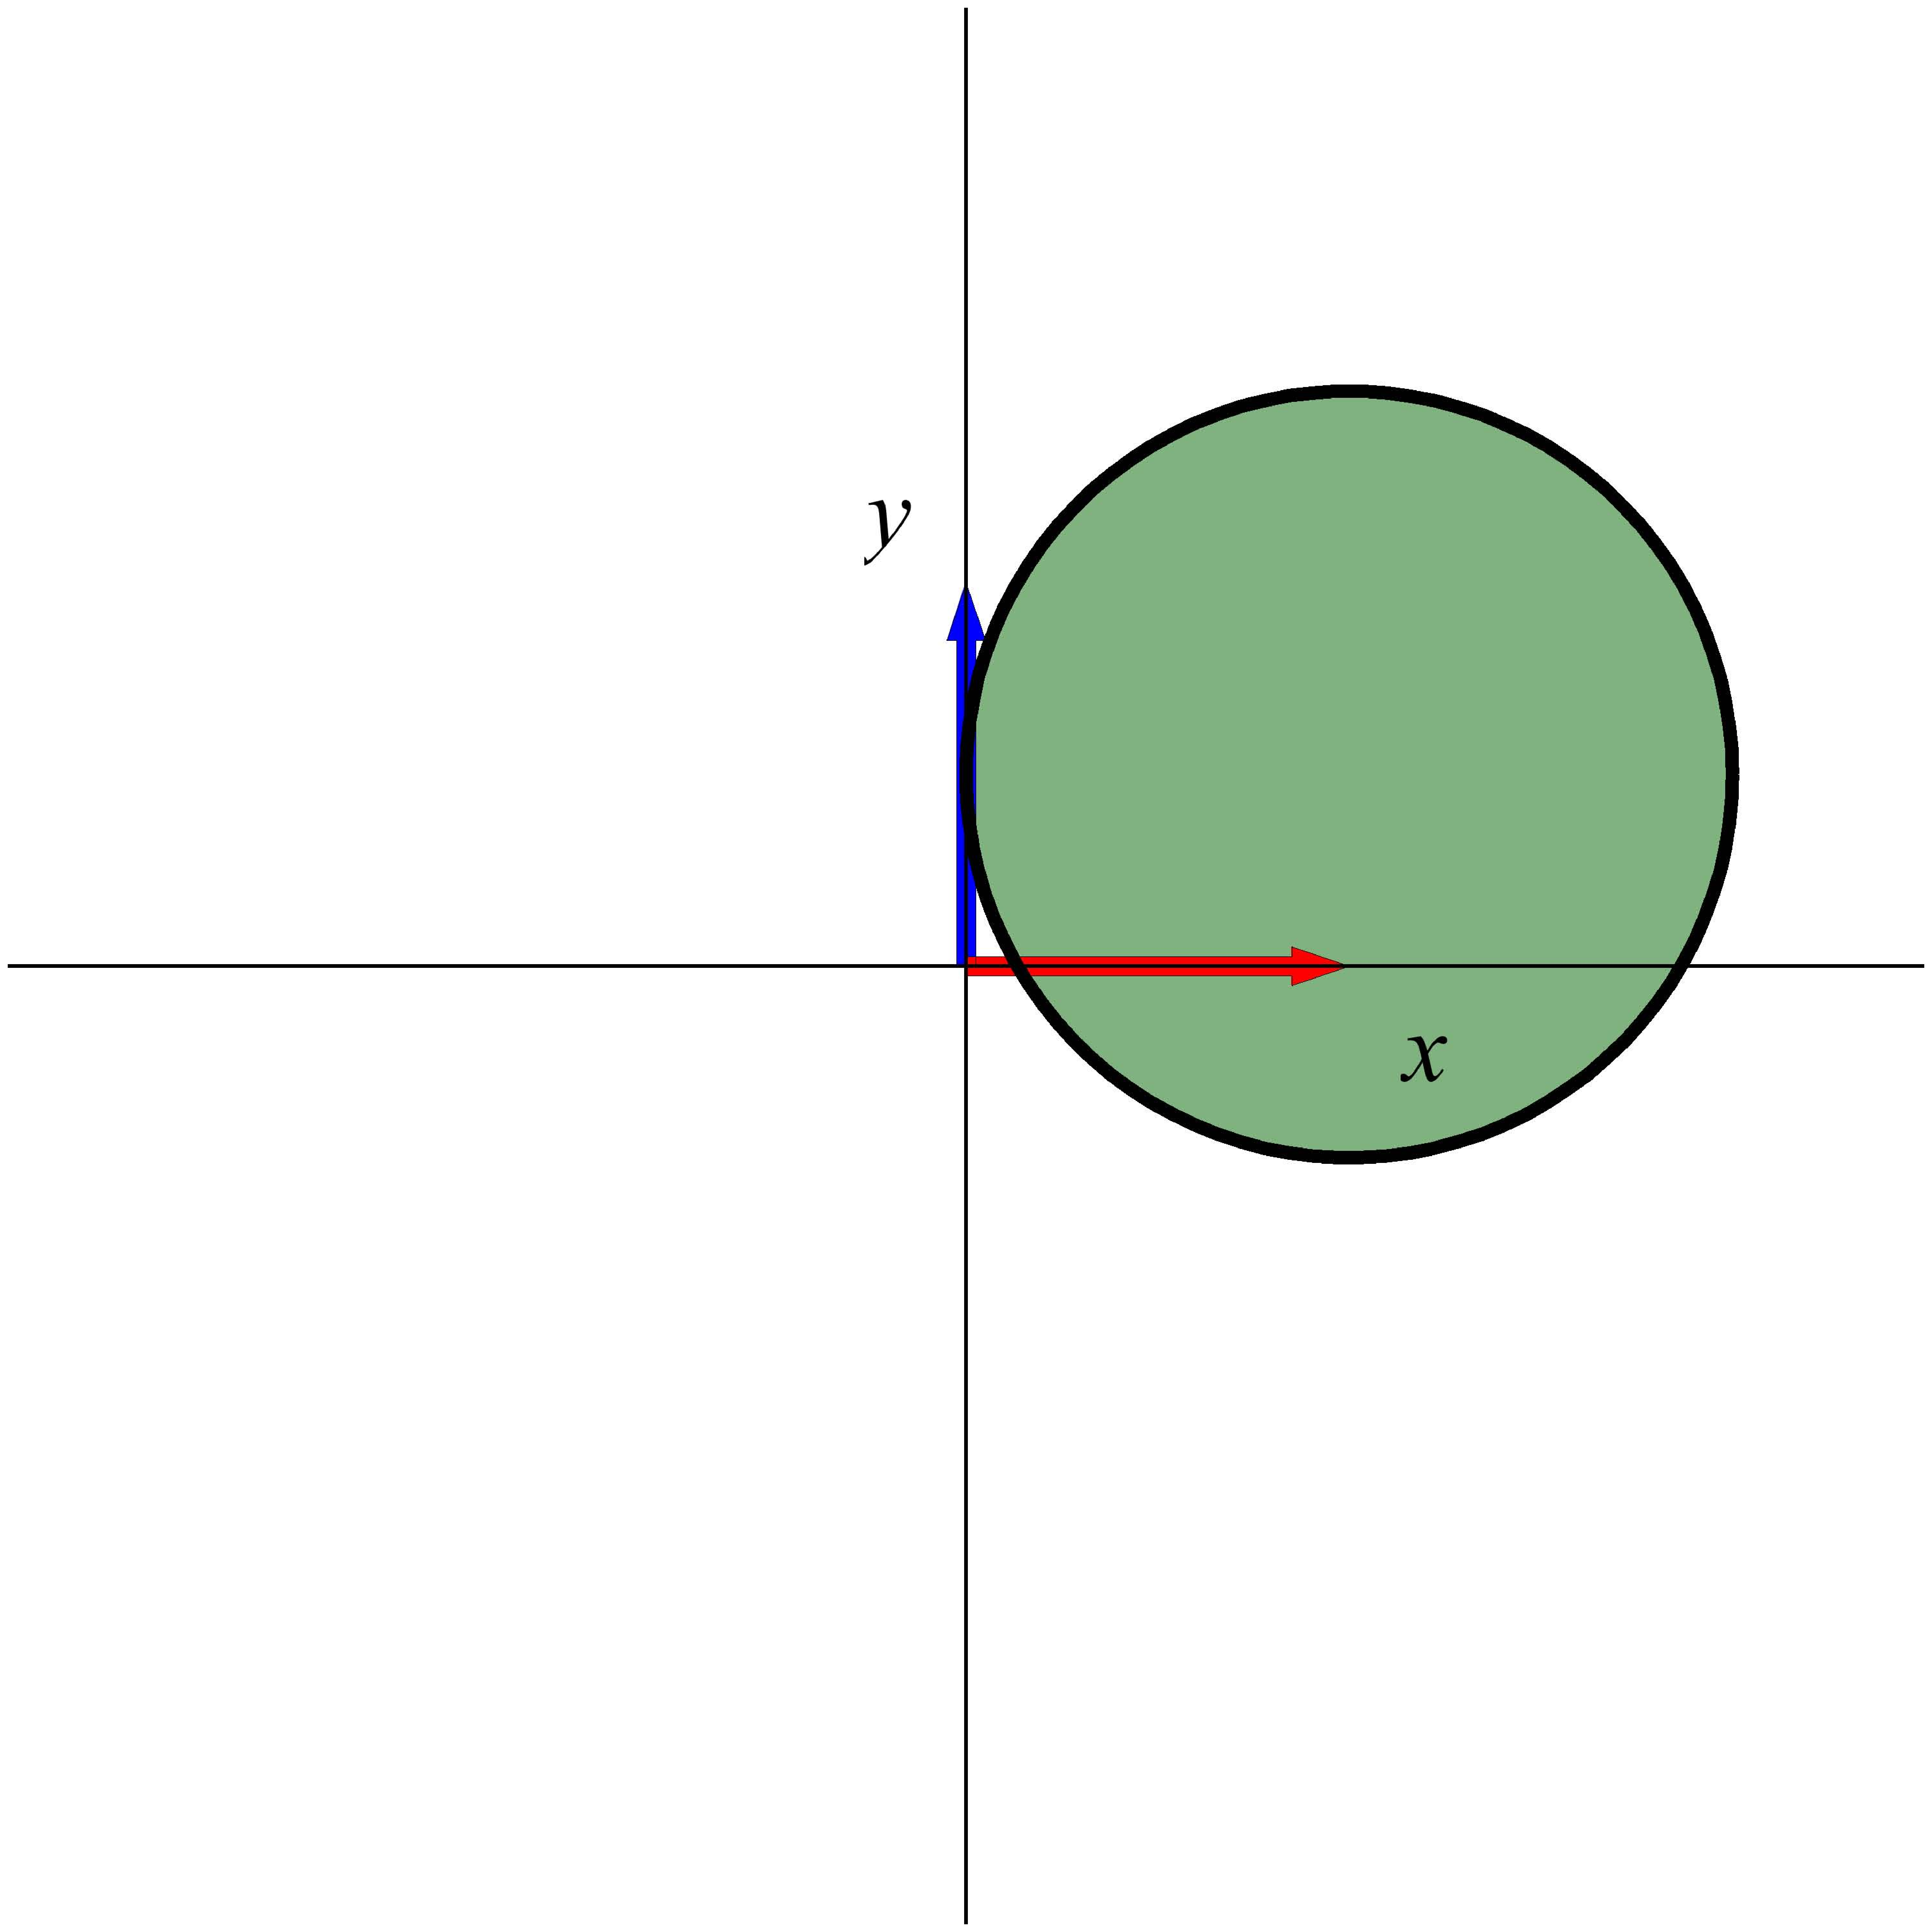
\includegraphics[height=55mm]{plotAfs2.pdf}\quad 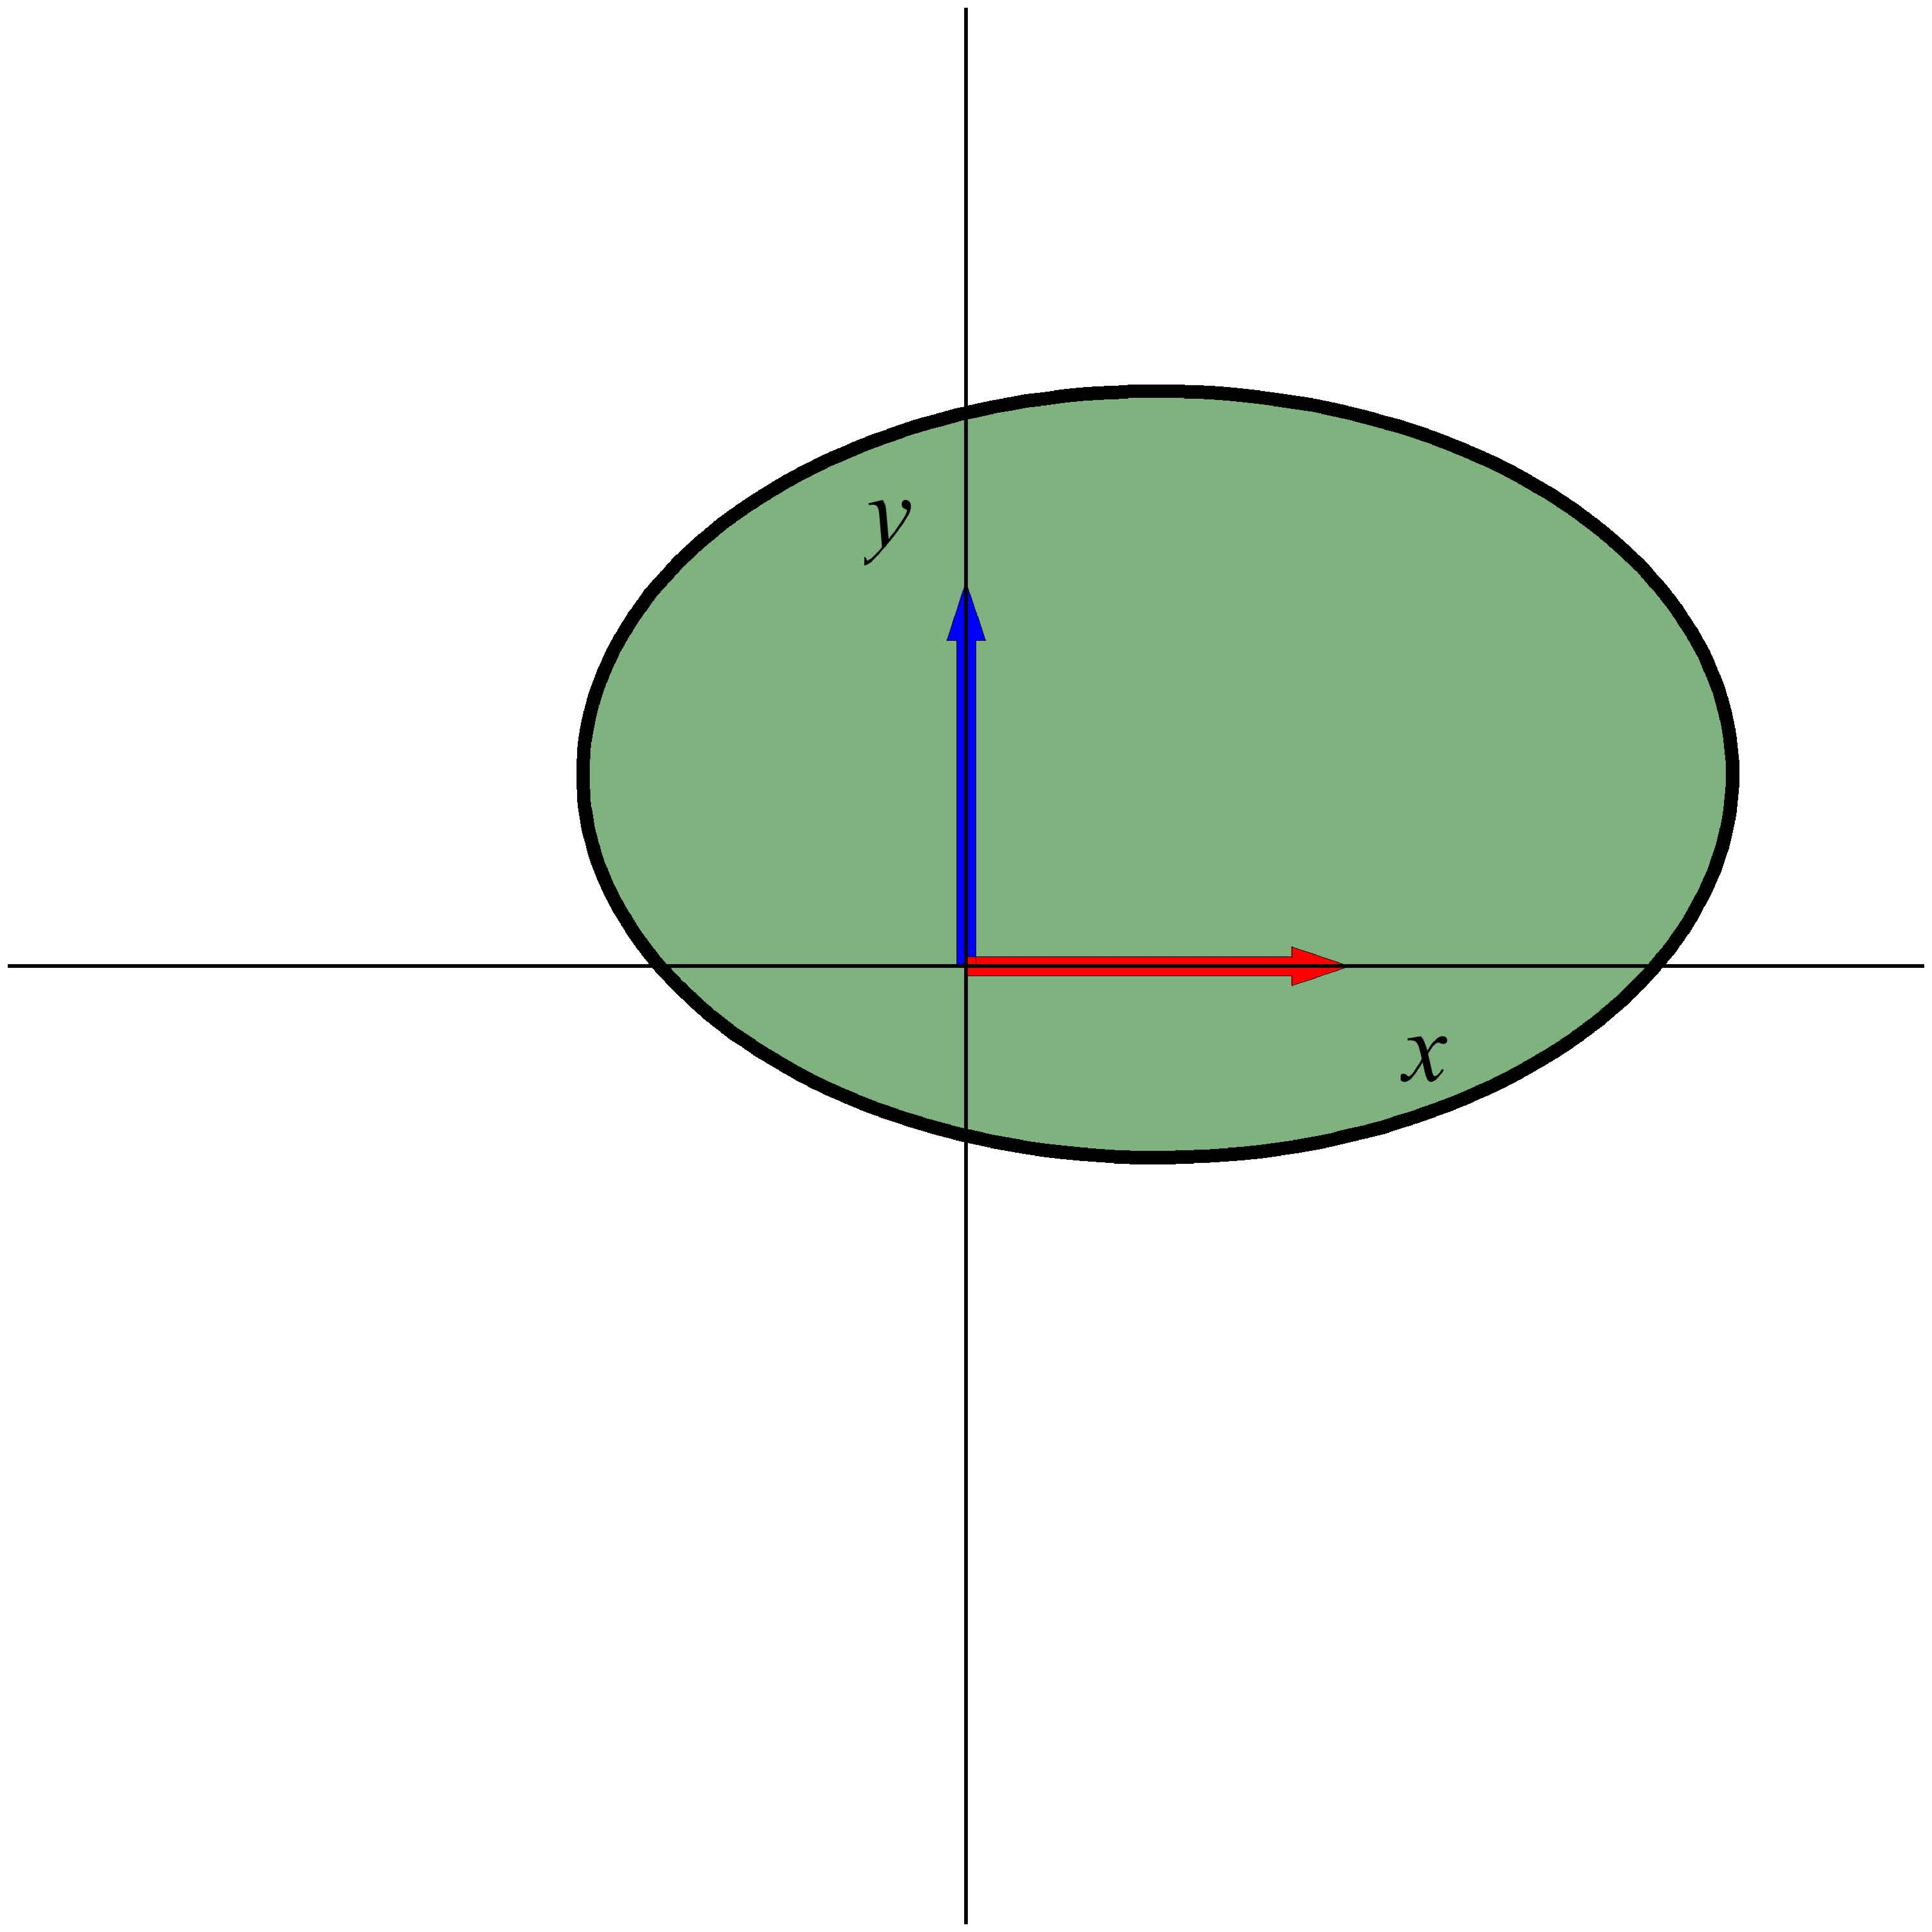
\includegraphics[height=55mm]{plotAfs3.pdf}}
\begin{center}
\caption{Afslutningerne  $\bar{A}$, $\bar{B}$, og $\bar{C}$ af områderne $A$, $B$, og $C$ fra figur \ref{figDefMgd}.} \label{figDefMgdAfs}
\end{center}
\end{figure}



\subsection{Stjerneformede mængder i planen}

\begin{definition}[Stjerneformede områder]
Hvis ethvert punkt $(x, y)$ i en mængde $M$ i planen kan 'ses' fra et punkt $(x_{0}, y_{0})$ i mængden sådan at hele syns-linjestykket fra og med $(x_{0}, y_{0})$ til og med $(x,y)$ er indeholdt i mængden, så siges $M$ at være \ind{stjerneformet mængde}{stjerneformet} ud fra \ind{stjernepunkt}{stjernepunktet} $(x_{0}, y_{0})$.  Med andre ord: Ethvert punkt $(x,y)$ i mængden kan forbindes med stjernepunktet med et linjestykke, der helt er indeholdt i mængden. Se figur \ref{figStjerner}.
\end{definition}

\begin{exercise}[Stjerneform og dobbelt-stjerneform]
Hvilke punkter i den mængde der er vist til venstre figur \ref{figStjerner} kan bruges som stjernepunkter for mængden? Er mængden af samtlige mulige stjernepunkter afsluttet eller åben? I hvilken forstand ville man kunne sige, at figuren til højre i  \ref{figStjerner} er \emph{dobbelt}-stjerneformet?
\end{exercise}


\begin{figure}[h]
\centerline{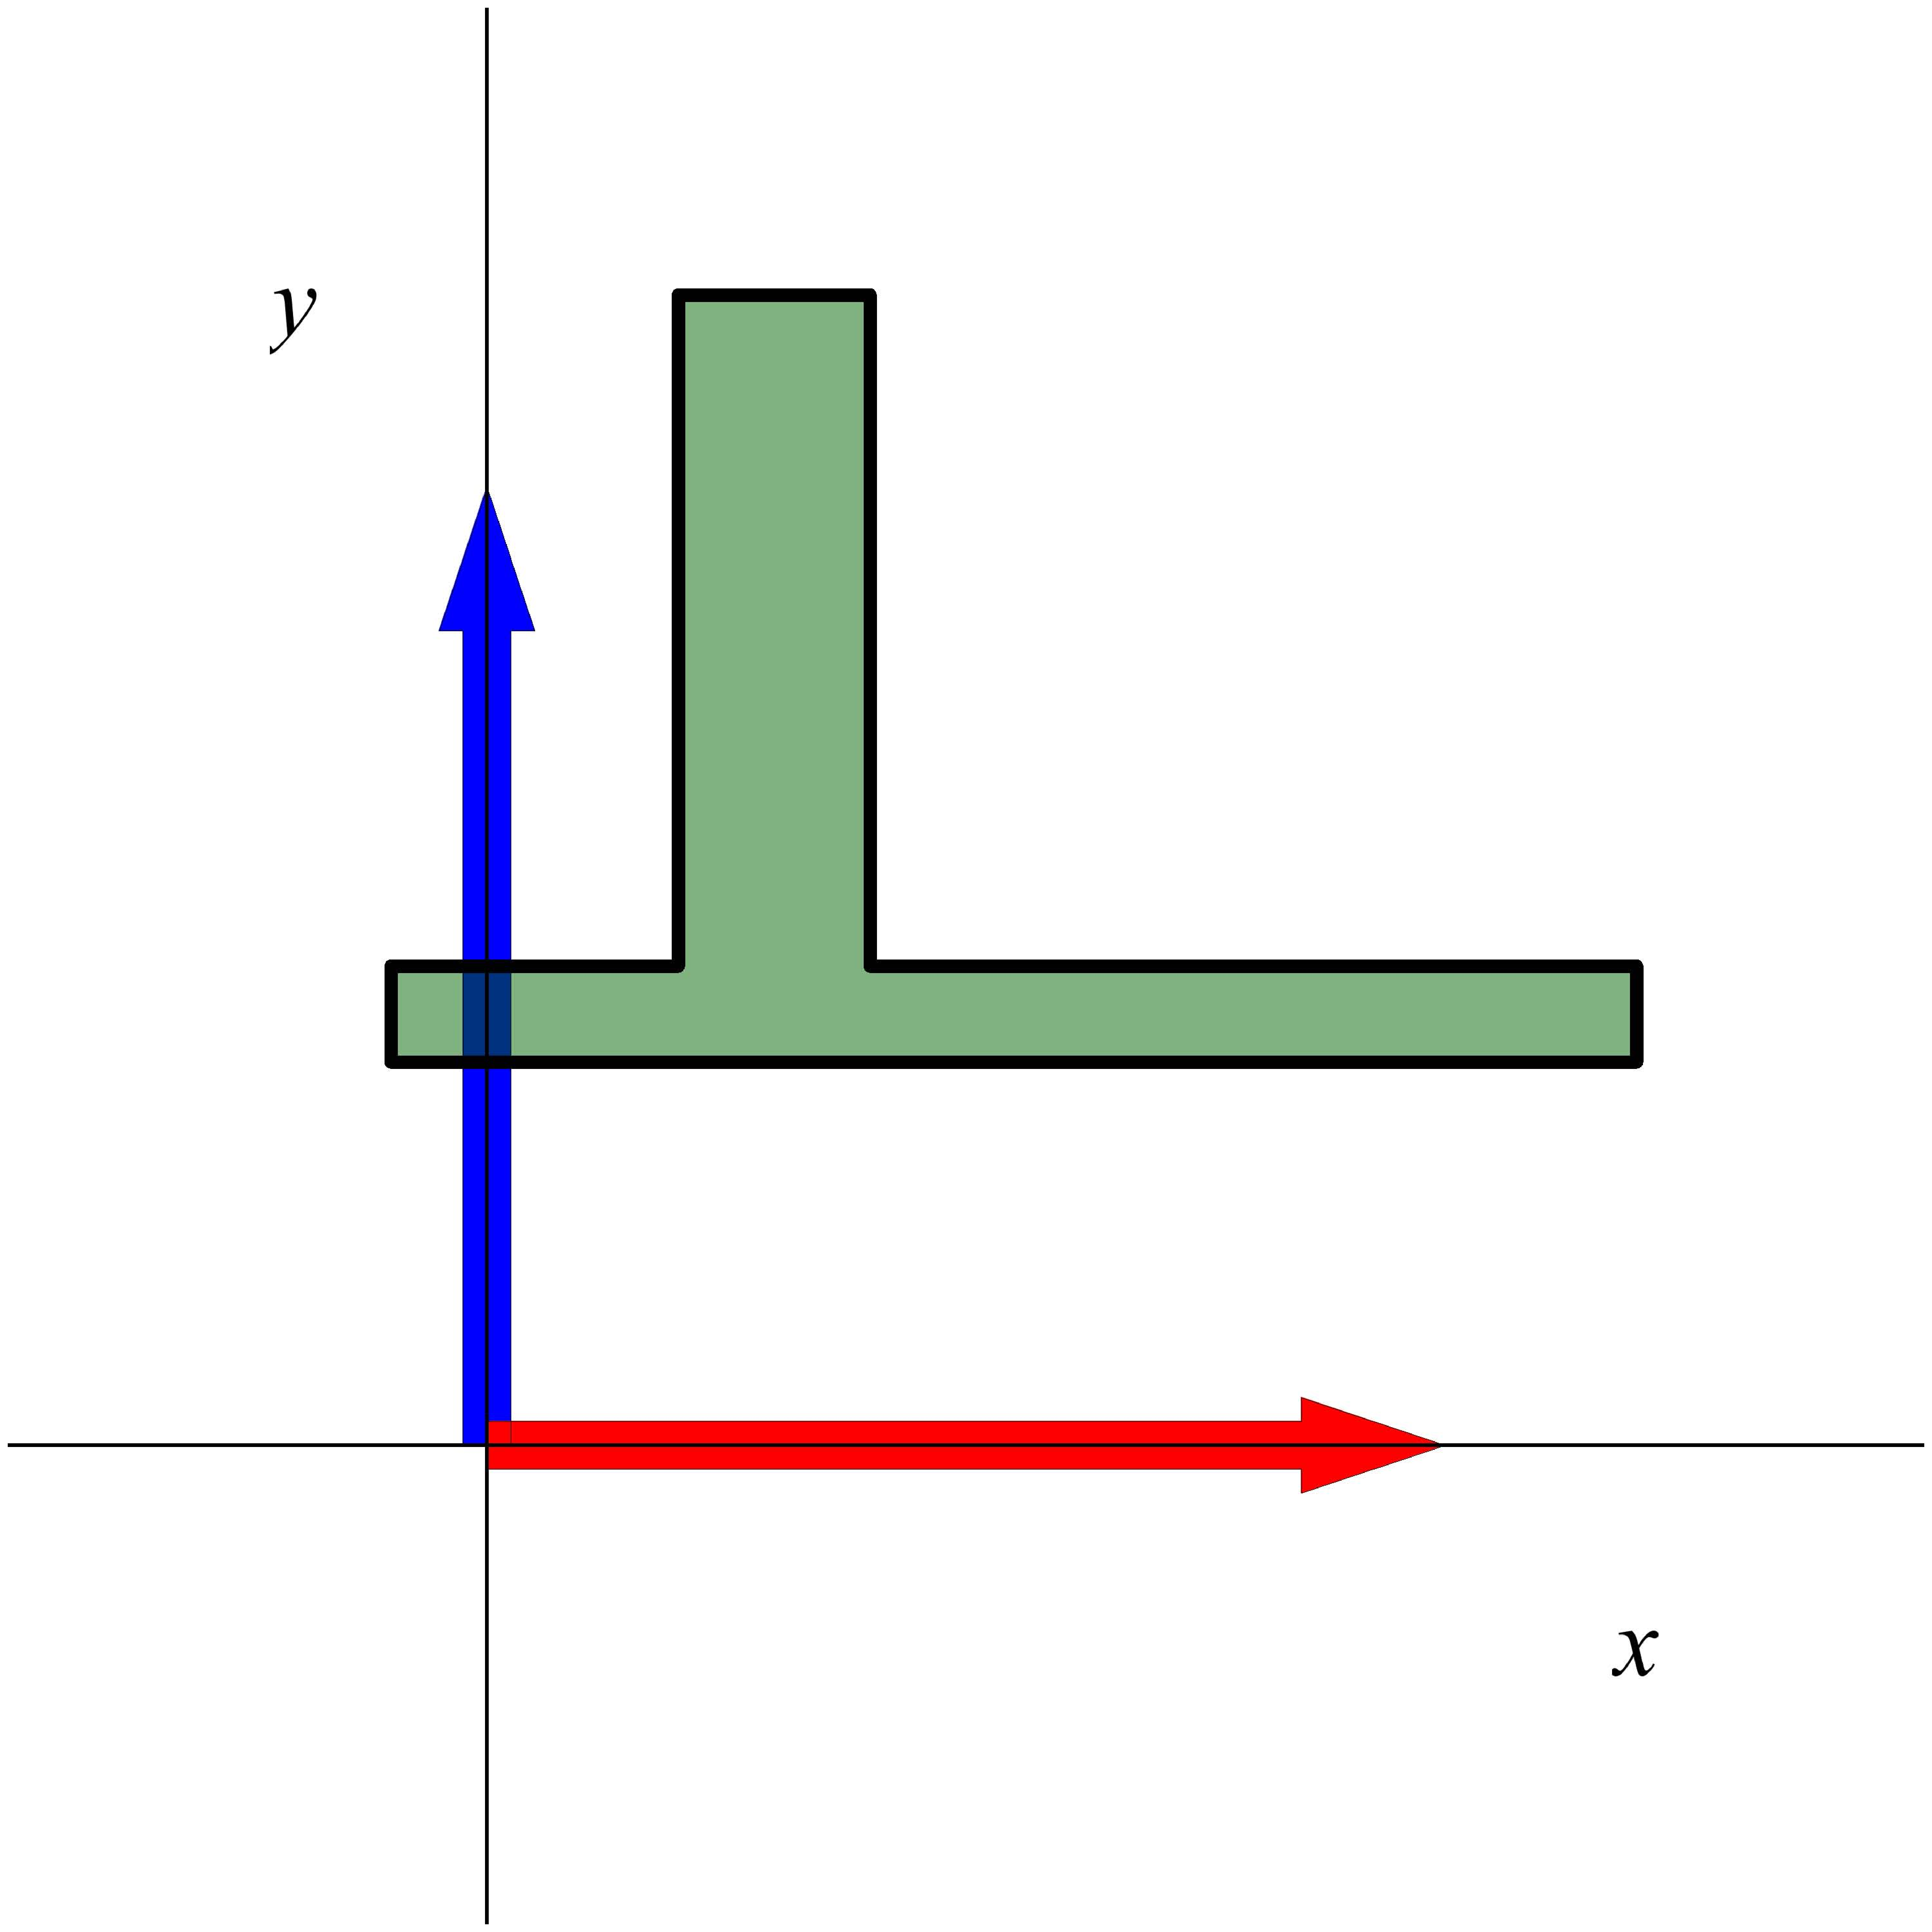
\includegraphics[height=55mm]{plotStjerne.pdf} \quad 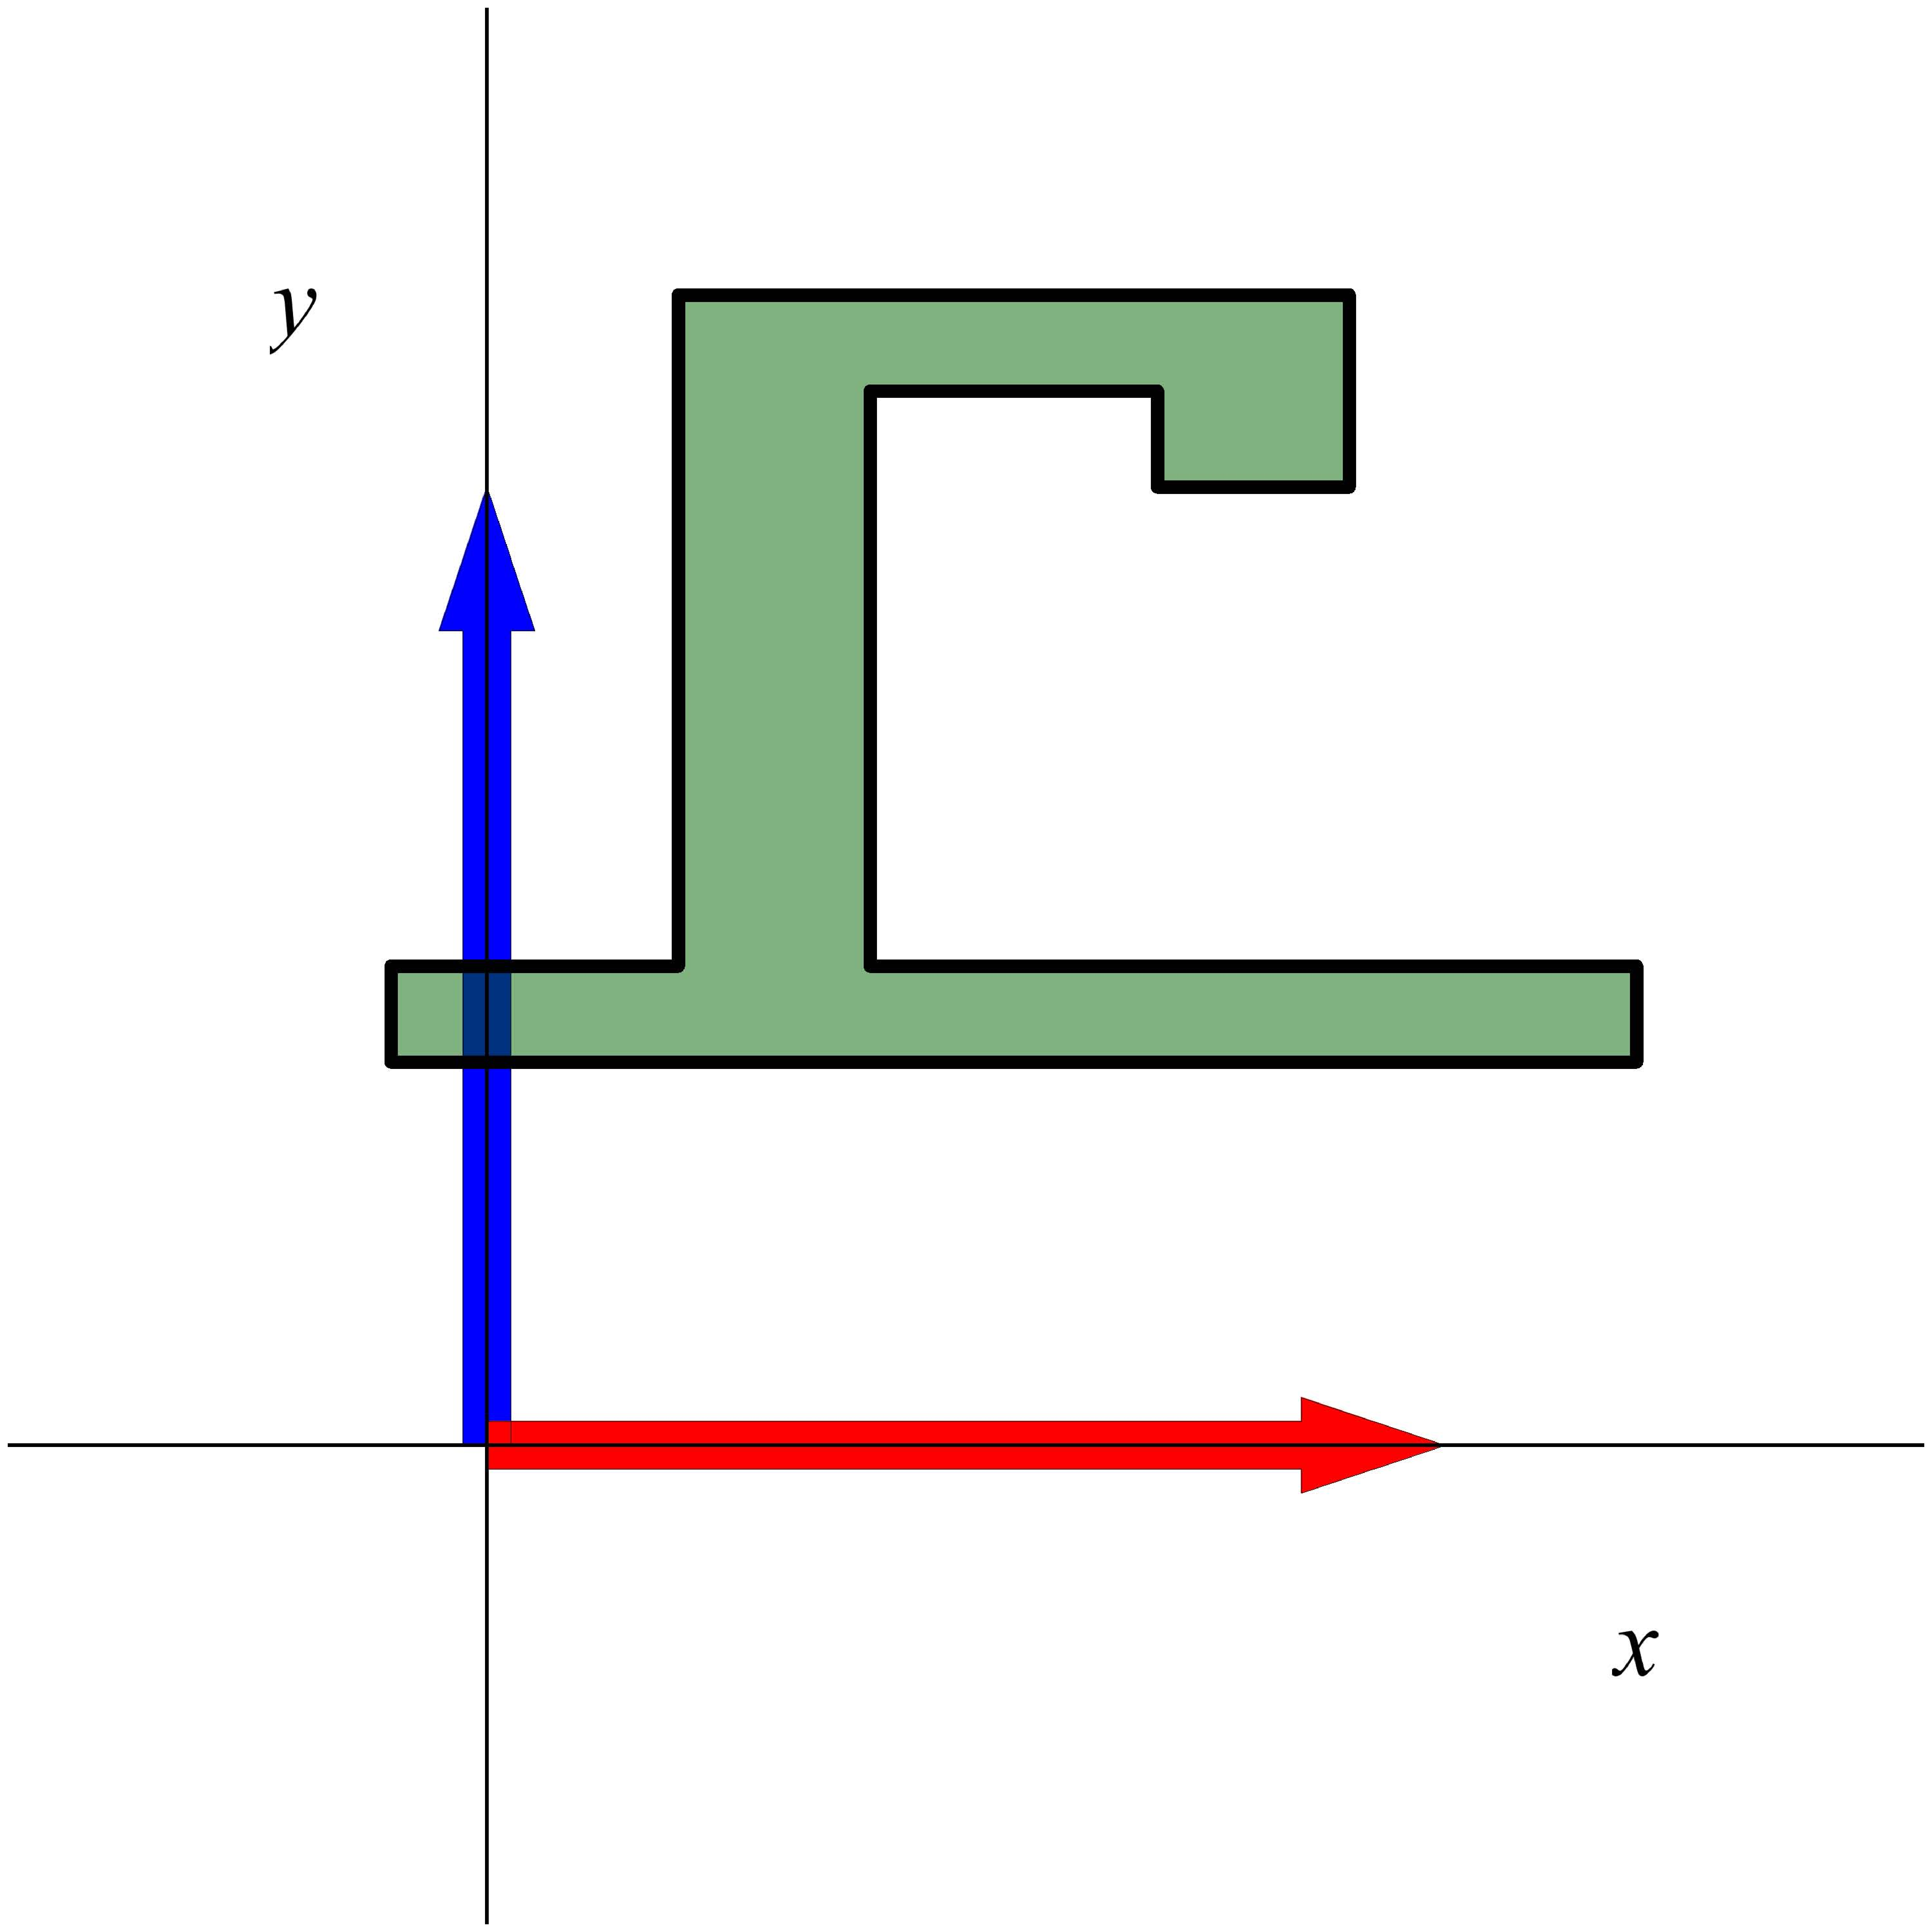
\includegraphics[height=55mm]{plotStjerneNon.pdf}}
\begin{center}
\caption{Mængden til venstre er stjerneformet. Mængden til højre er \emph{ikke} stjerneformet.} \label{figStjerner}
\end{center}
\end{figure}

\subsection{Begrænsede mængder i planen}
\begin{definition}[Begrænsede mængder]
En mængde $M$ i planen siges at være \ind{begrænset mængde}{begrænset} hvis den er helt indeholdt i en (gerne meget stor) cirkelskive med centrum i $(0,0)$.
\end{definition}

\begin{example}
De tre mængder $A$, $B$, og $C$ i figur \ref{figDefMgd} er tydeligvis begrænsede -- de er helt indeholdt i den cirkelskive som har centrum i $(0,0)$ og radius $100$. Den mængde af punkter, der udgøres af punkterne på $x$-aksen er ikke begrænset.
\end{example}


\subsection[Udvidelser af definitionsmængden til hele planen]{Udvidelser af definitionsmængden til hele $\mathbb{R}^{2}$}
Ligesom vi kan udvide definitionsmængder for funktioner af \'{e}n variabel, kan vi gøre præcis det samme for funktioner $f(x,y)$ af to variable:

\begin{definition}[Udvidelse af definitionsmængden]
Givet funktionen $f(x,y)$ med definitionsmængde  $\mathcal{D}m(f)$, så definerer vi
$0$-udvidelsen $\widehat{f}(x,y)$ af  $f(x,y)$ på følgende måde:
\begin{equation}
\widehat{f}(x,y) = \left\{
                      \begin{array}{ll}
                        f(x,y)\, , & \hbox{for} \quad (x, y) \in \mathcal{D}m(f)\\
                        0 \, , & \hbox{for} \quad  (x,y) \in \mathbb{R}^{2} \setminus \mathcal{D}m(f) \quad .
                      \end{array}
                    \right.
\end{equation}
\end{definition}

\section{Grafer for funktioner af to variable}
Med henblik på at illustrere funktioner af to variable tegner vi dem  i rummet -- vi plotter den punktmængde, der fremkommer ved at konstruere graferne  i $\{\,\mathcal{O}, x, y, z\,\}$-koordinatsystemet:

\begin{definition}[Grafer for funktioner af to variable]
Lad $f(x,y)$ være en funktion af to variable med definitionsmængden $\mathcal{D}m(f)$. Så er \ind{grafen for funktionen}{grafen for en funktion af to variable} givet ved:
\begin{equation}
z = f(x,y) \quad , \quad \textrm{hvor} \quad (x,y) \in \mathcal{D}m(f) \quad .
\end{equation}
Grafen består altså af den punktmængde i rummet som vi også kan beskrive på følgende måde:
\begin{equation}
\mathcal{G}(f) = \maengde{(x,y,f(x,y))}{(x,y) \in \mathcal{D}m(f)} \quad .
\end{equation}
Hvert enkelt punkt på grafen fremkommer på følgende måde:  Fra punktet $(x,y,0)$ i $(x, y)$-planen
går vi højden (med fortegn) $f(x,y)$ lodret op (eller ned) fra den (vandrette) $(x, y)$-plan og markere graf-punktet $(x, y, f(x,y)$ i den højde som funktionsværdien $f(x,y)$ foreskriver -- lige over (eller under) punktet $(x,y,0)$.
\end{definition}



\section{Niveau-mængder og højdesnit}
I $(x,y)$-planen hvor funktionen $f(x,y)$ er defineret kan vi gøre noget helt andet for at vise, hvordan funktionsværdierne varierer fra punkt til punkt.

\begin{definition}[Niveau-mængder]
For en funktion $f(x,y)$ af to variable definerer vi for ethvert reelt tal $c$ den tilhørende \ind{niveau-mængde}{niveau-mængde} på følgende måde:
\begin{equation}
\mathcal{K}_{c}(f) = \maengde{(x,y) \in \mathcal{D}m(f)}{f(x,y) = c} \quad .
\end{equation}
\end{definition}


Mængden $\mathcal{K}_{c}$ kan være tom, hele planen, en kurve,  eller hvilken som helst punktmængde i planen.


\begin{example}[Niveaumængder]
Vi lader $A$ betegne en vilkårlig mængde i planen og  konstruerer en funktion $f(x,y)$ i hele planen på følgende måde:
\begin{equation}
f(x,y) = \left\{
           \begin{array}{ll}
             1 & \hbox{\,\,for $(x,y) \in A$} \\
             0 & \hbox{\,\,for $(x,y) \in \mathbb{R}^{2} \setminus A$\quad ,}
           \end{array}
         \right.
\end{equation}
dvs. $f$ er $0$-udvidelsen af den funktion, som er konstant $1$ på $A$. Så er
\begin{equation}
\mathcal{K}_{c}(f) = \left\{
  \begin{array}{ll}
    A & \hbox{\,\,for $c = 1$} \\
    \mathbb{R}^{2} \setminus A & \hbox{\,\,for $c = 0$} \\
    \emptyset  & \hbox{\,\,for $c \neq 1$ og $c \neq 0$\quad .}
  \end{array}
\right.
\end{equation}
\end{example}

Ofte er niveau-mængden $\mathcal{K}_{c}$ dog meget mere velstruktureret og består typisk af en eller flere kurver.
De kurver kan med fuld ret kaldes niveau-kurver eller højdekurver, for de angiver jo præcis de punkter $(x,y)$ i definitionsmængden hvor funktionen antager værdien $c$ og hvor grafen for $f$ derfor lige præcis har højden (med fortegn) $c$ over $(x,y)$-planen. Med andre ord, hvis vi skærer
grafen for $f$ med den vandrette plan $z = c$ i højden $c$ over $(x,y)$-planen, så fås en snitkurve, hvis projektion ned i (eller op i)
$(x,y)$-planen netop er $\mathcal{K}_{c}$, se figurerne \ref{figLin} \ref{figCosSin}, \ref{figParab}.




\begin{think}
Nedenfor i afsnit \ref{subsecGradientVec}  vil vi i ethvert punkt i definitionsmængden for $f(x,y)$ definere en vektor, gradientvektoren for $f(x,y)$, som har den særlige egenskab, at hvis den ikke er $\mathbf{0}$ i et åbent område omkring et givet punkt $(x_{0}, y_{0})$,  så er den niveau-mængde der indeholder $(x_{0}, y_{0})$ en kurve igennem punktet. Gradientvektorer er dog kun veldefinerede for differentiable funktioner, så den egenskab må vi derfor først have indført forfunktioner af to variable.
\end{think}

\begin{example}[Grafer og niveau-kurver]
Følgende funktioner er alle definerede i hele $(x,y)$-planen.
\begin{equation}
\begin{aligned}
f(x,y) &= -x + y + 2 \\
f(x,y) &= 1- \frac{1}{2}\left(x^{2} + y^{2} \right) \\
f(x,y) &= \cos(3x)\cdot\sin(3y) \quad .
\end{aligned}
\end{equation}
Funktionernes grafer er vist i figurerne \ref{figLin}, \ref{figParab}, og \ref{figCosSin} dels sammen med deres respektive niveau-kurver i $(x,y)$-planen og dels sammen med en figur, der antyder, hvordan niveaukurverne i $(x,y)$-planen kan opfattes som projektionerne af de højde-snit-kurver der fremkommer ved at skære graffladerne for funktionerne i forskellige højder, altså med planerne $z = c$, hvor $c$ er den konstante værdi som den aktuelle funktion $f(x, y)$ antager på niveau-kurven $\mathcal{K}_{c}$. Bemærk, at niveaumængderne $\mathcal{K}_{c}$ virkelig \emph{er} kurver (eller punkter) i disse tilfælde.
\end{example}

\begin{figure}[h]
\centerline{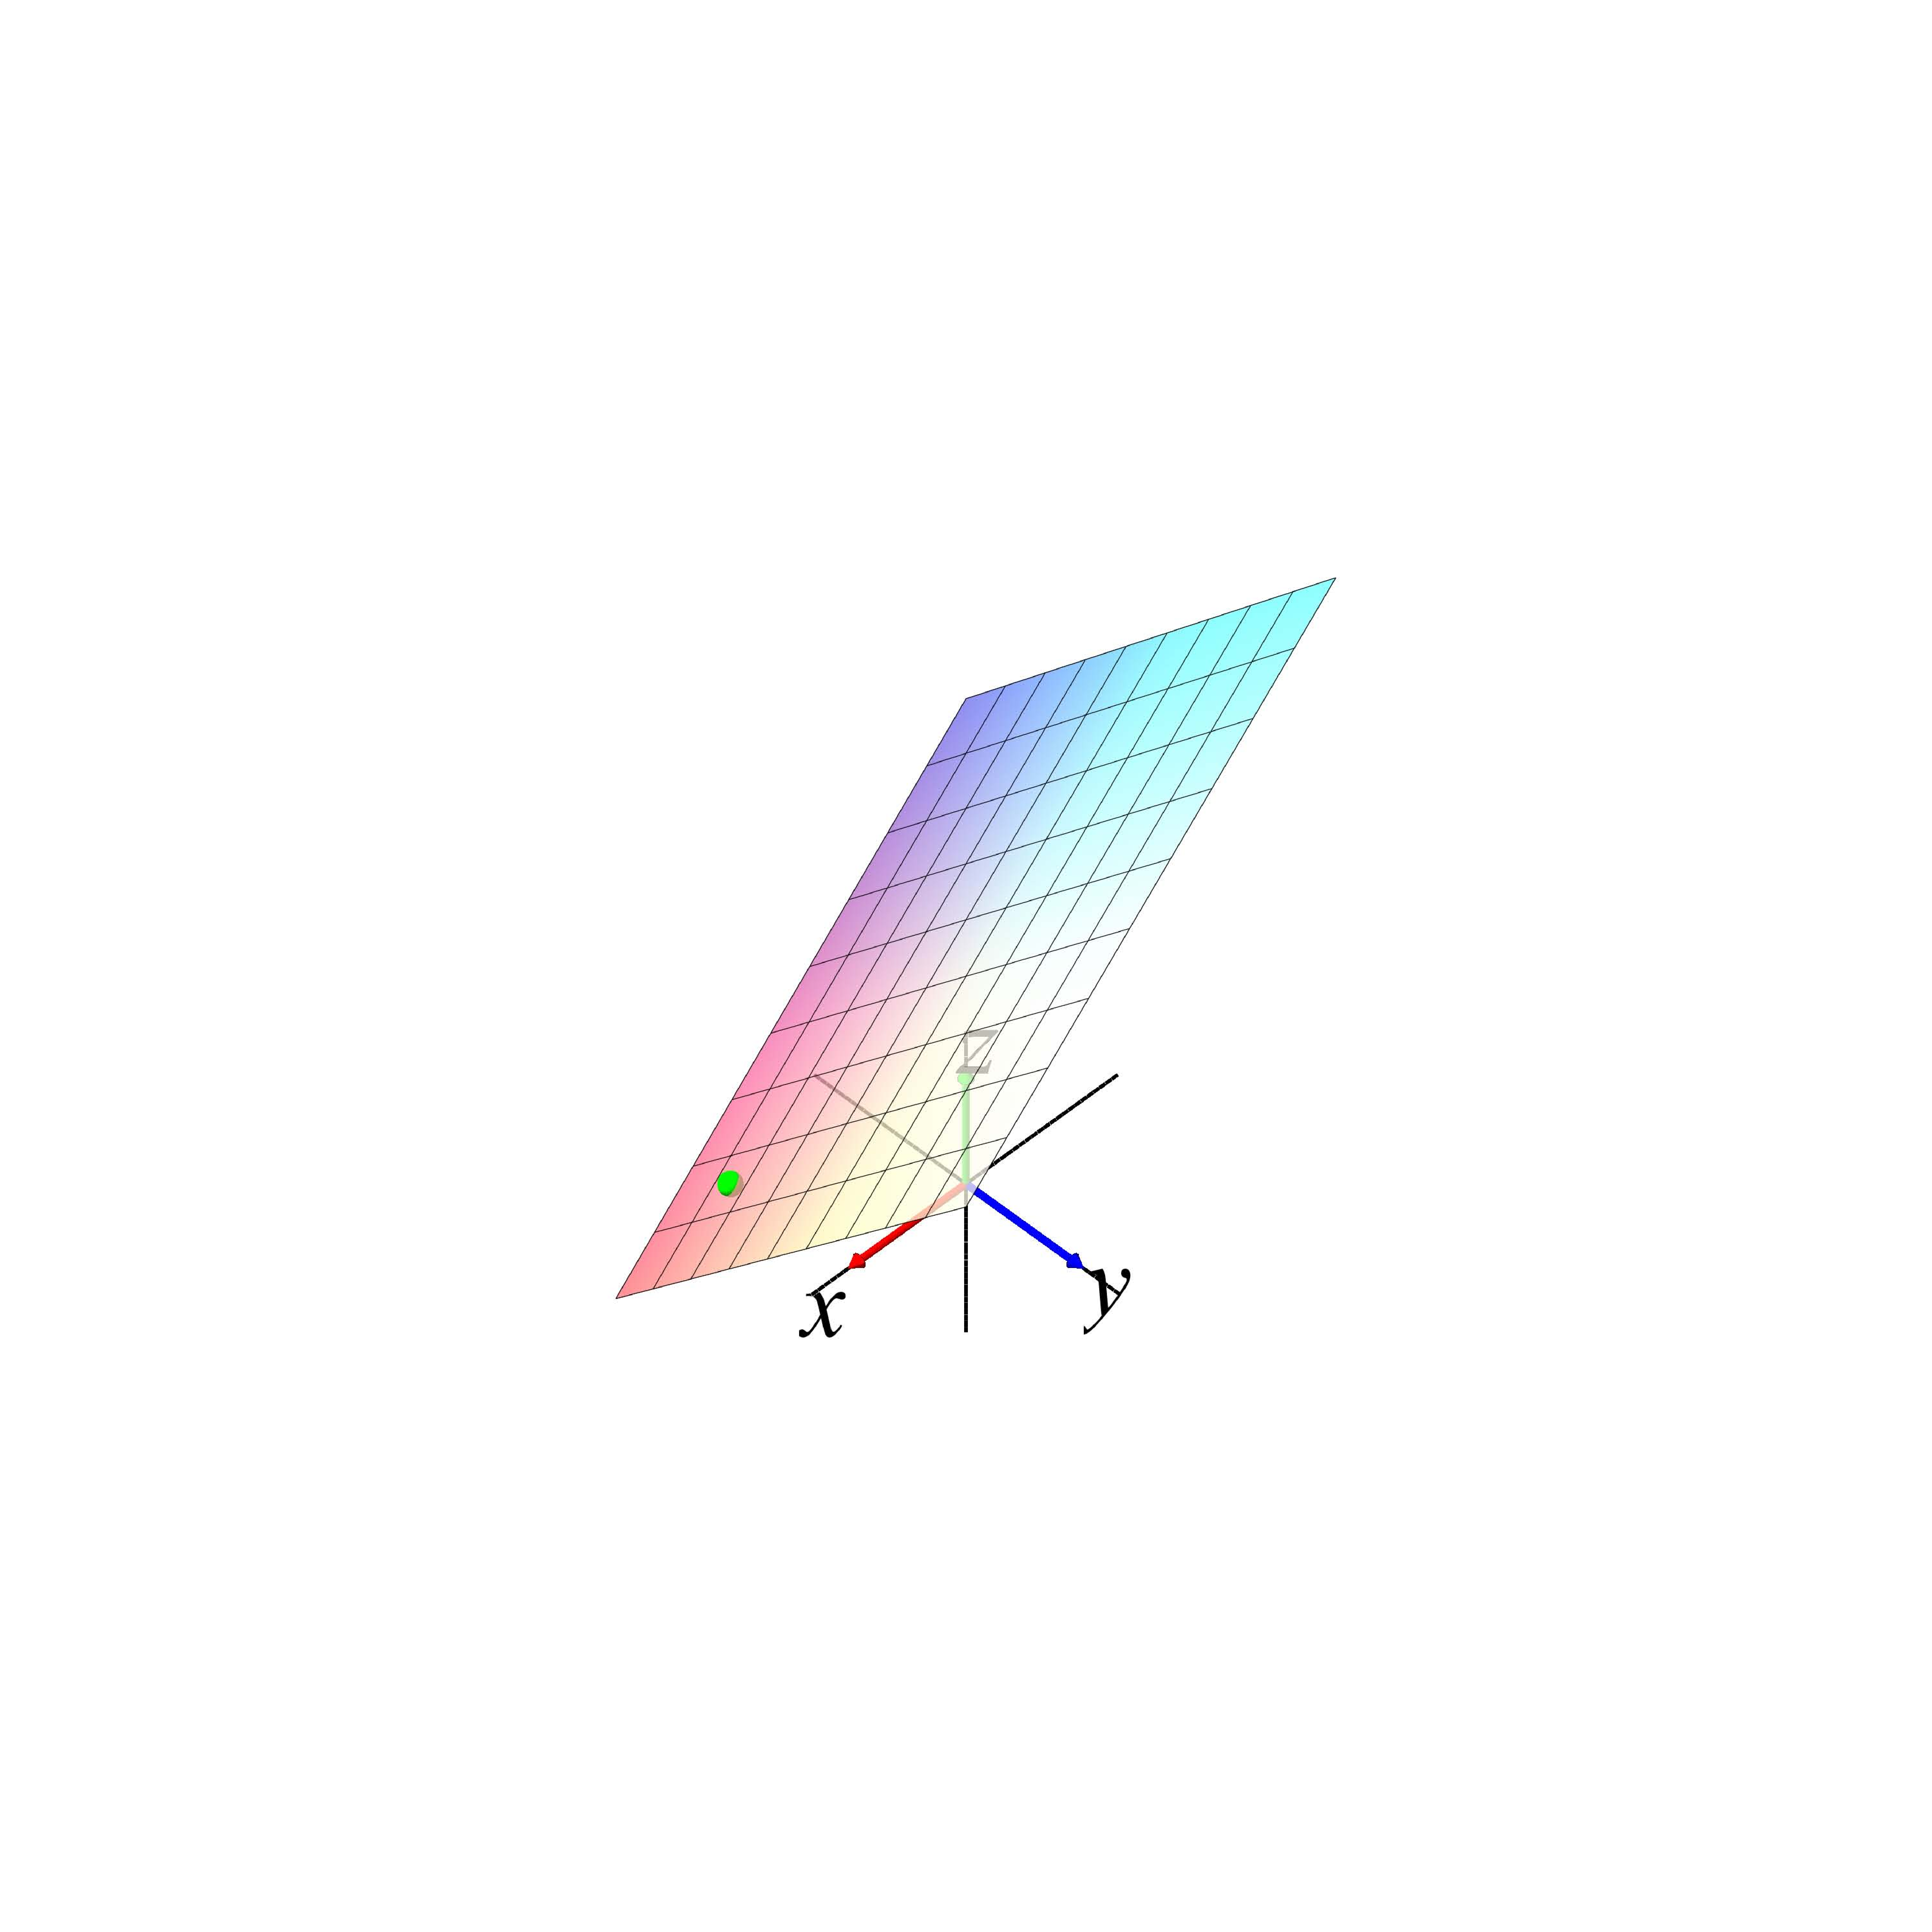
\includegraphics[height=80mm]{plotLin.pdf}\quad 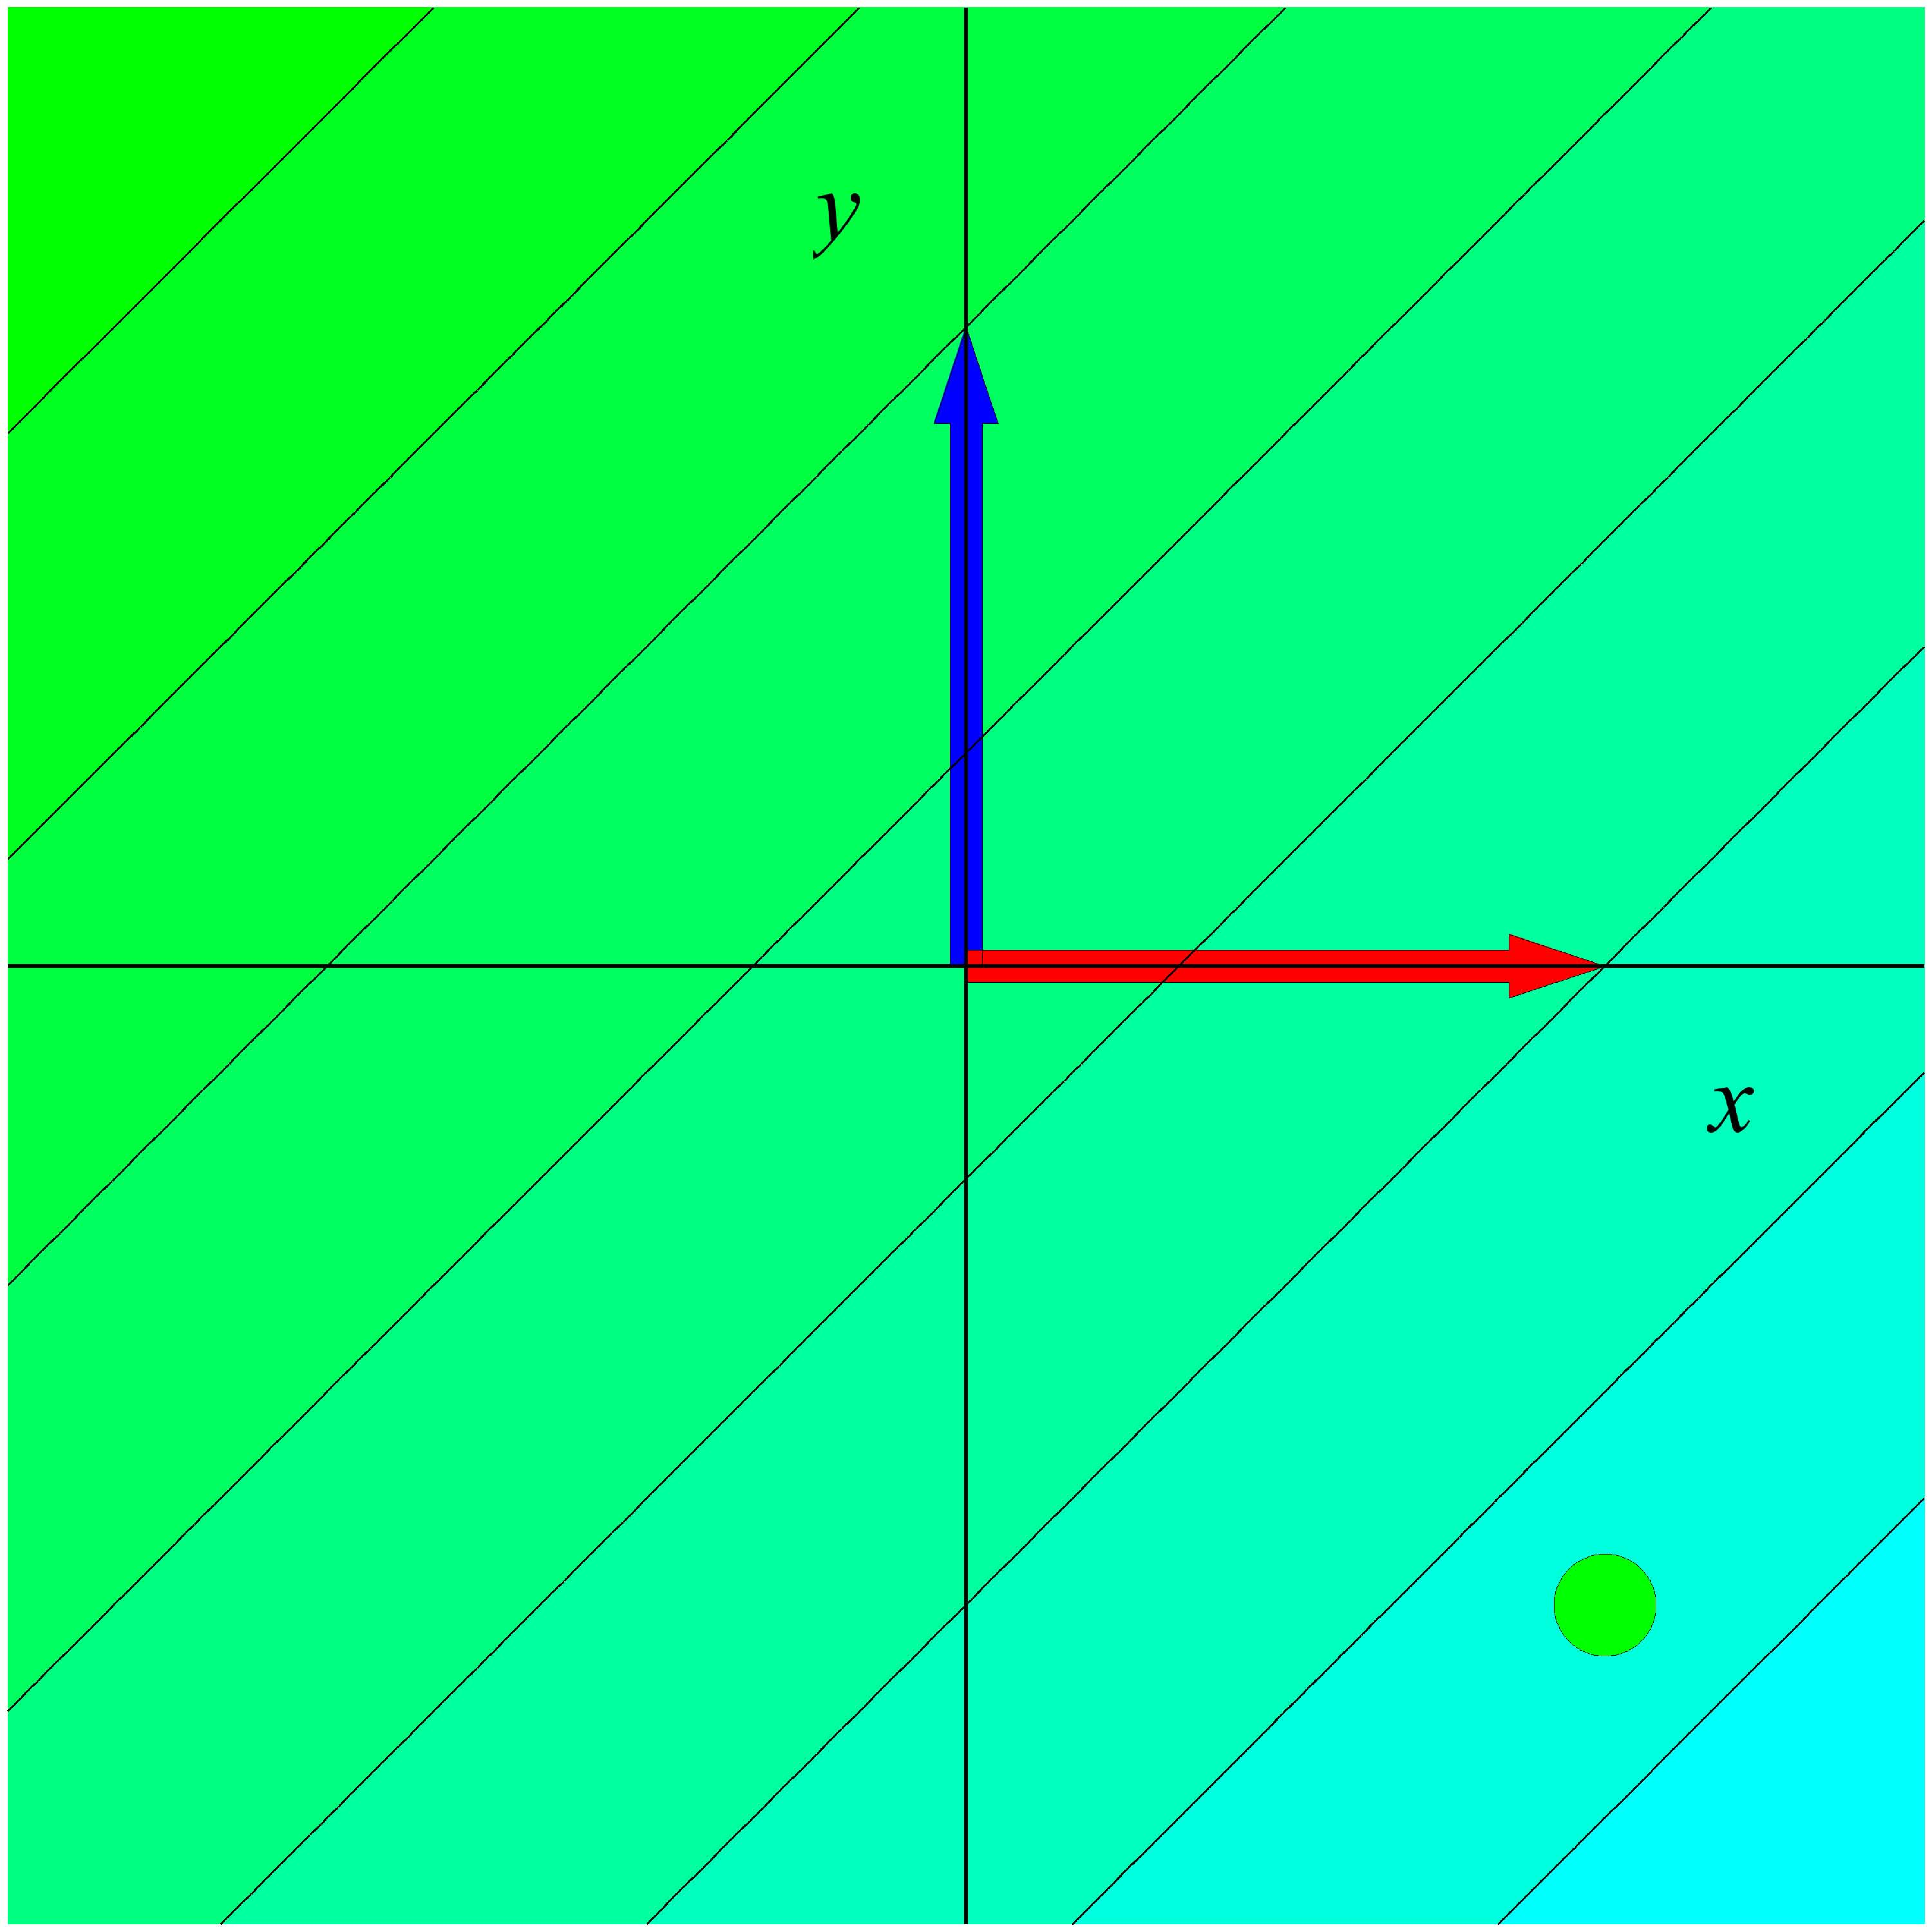
\includegraphics[height=25mm]{plotLinNiveau.pdf} \quad 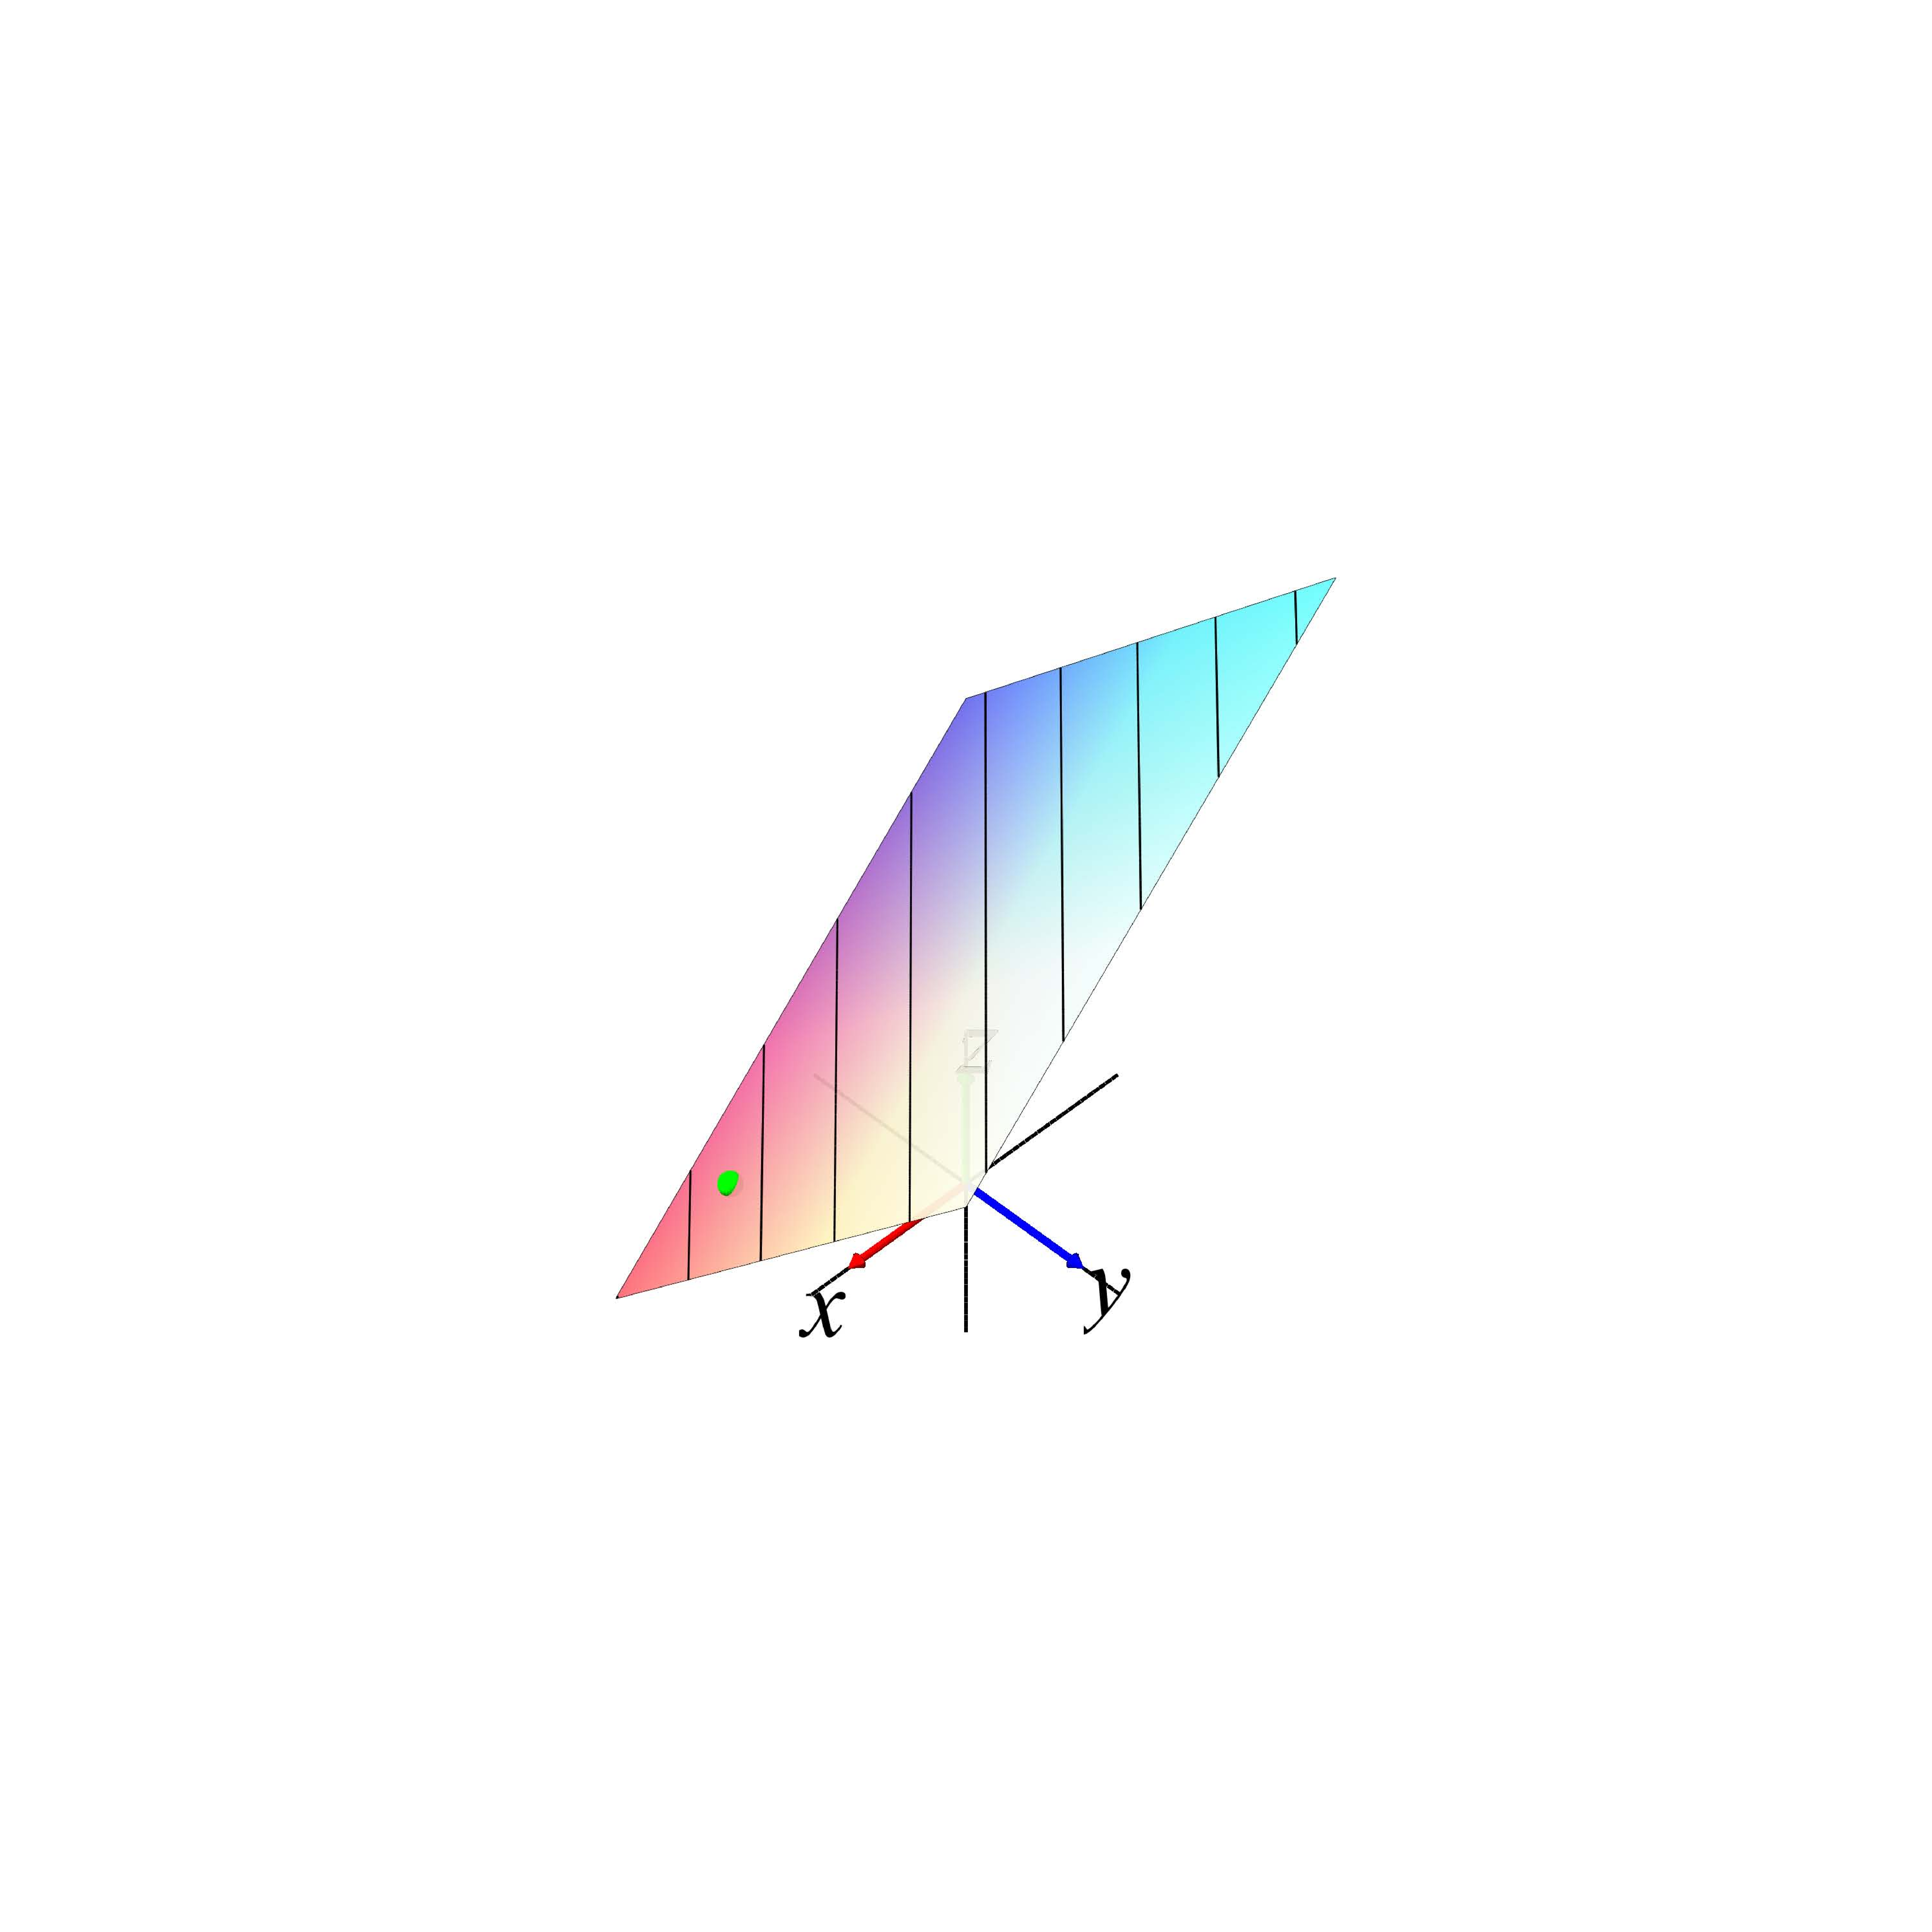
\includegraphics[height=80mm]{plotLinNiveauUP.pdf}}
\begin{center}
\caption{Grafen i $(x,y,z)$-rummet, niveaukurverne i $(x,y)$-planen, og højdesnitkurverne for funktionen $f(x,y) = -x + y + 2$. Læg mærke til, at det naturligvis ikke er \emph{hele} grafen for funktionen vi kan plotte. Her er kun vist det udsnit der hører til $-1 \leq x \leq 1$ og $-1 \leq y \leq 1$.} \label{figLin}
\end{center}
\end{figure}


\begin{figure}[h]
\centerline{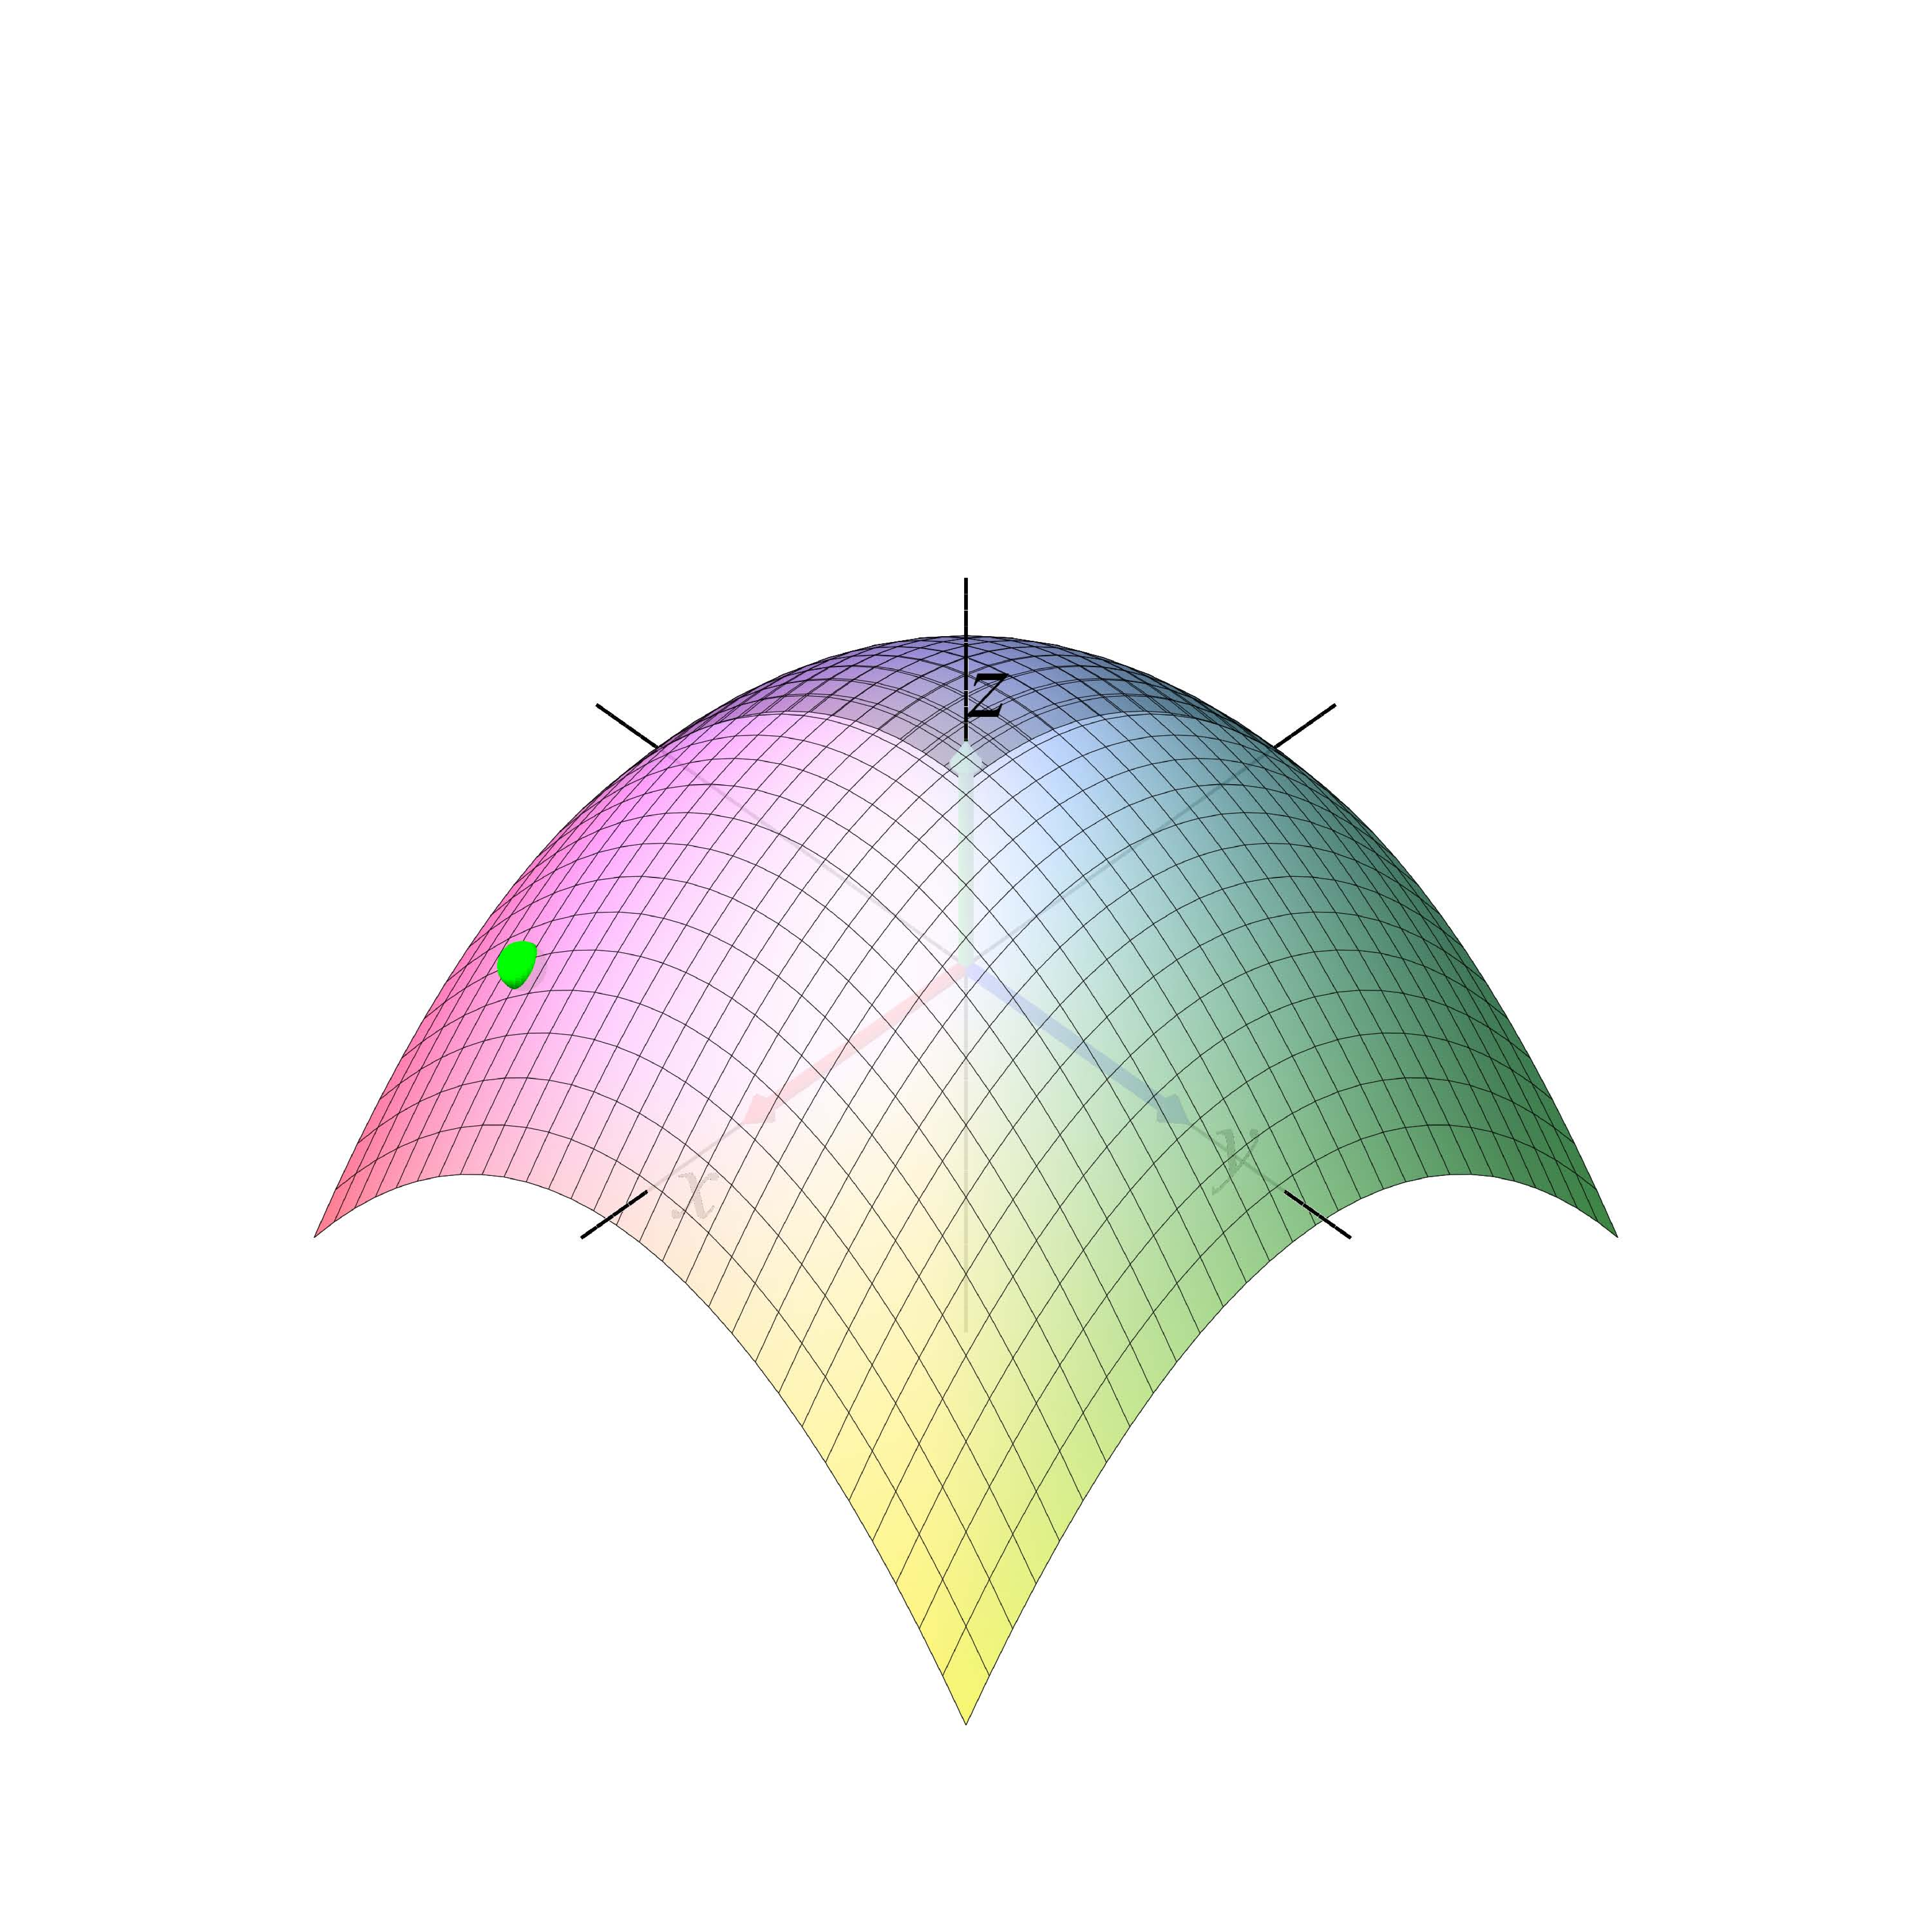
\includegraphics[height=80mm]{plotParab.pdf}\quad 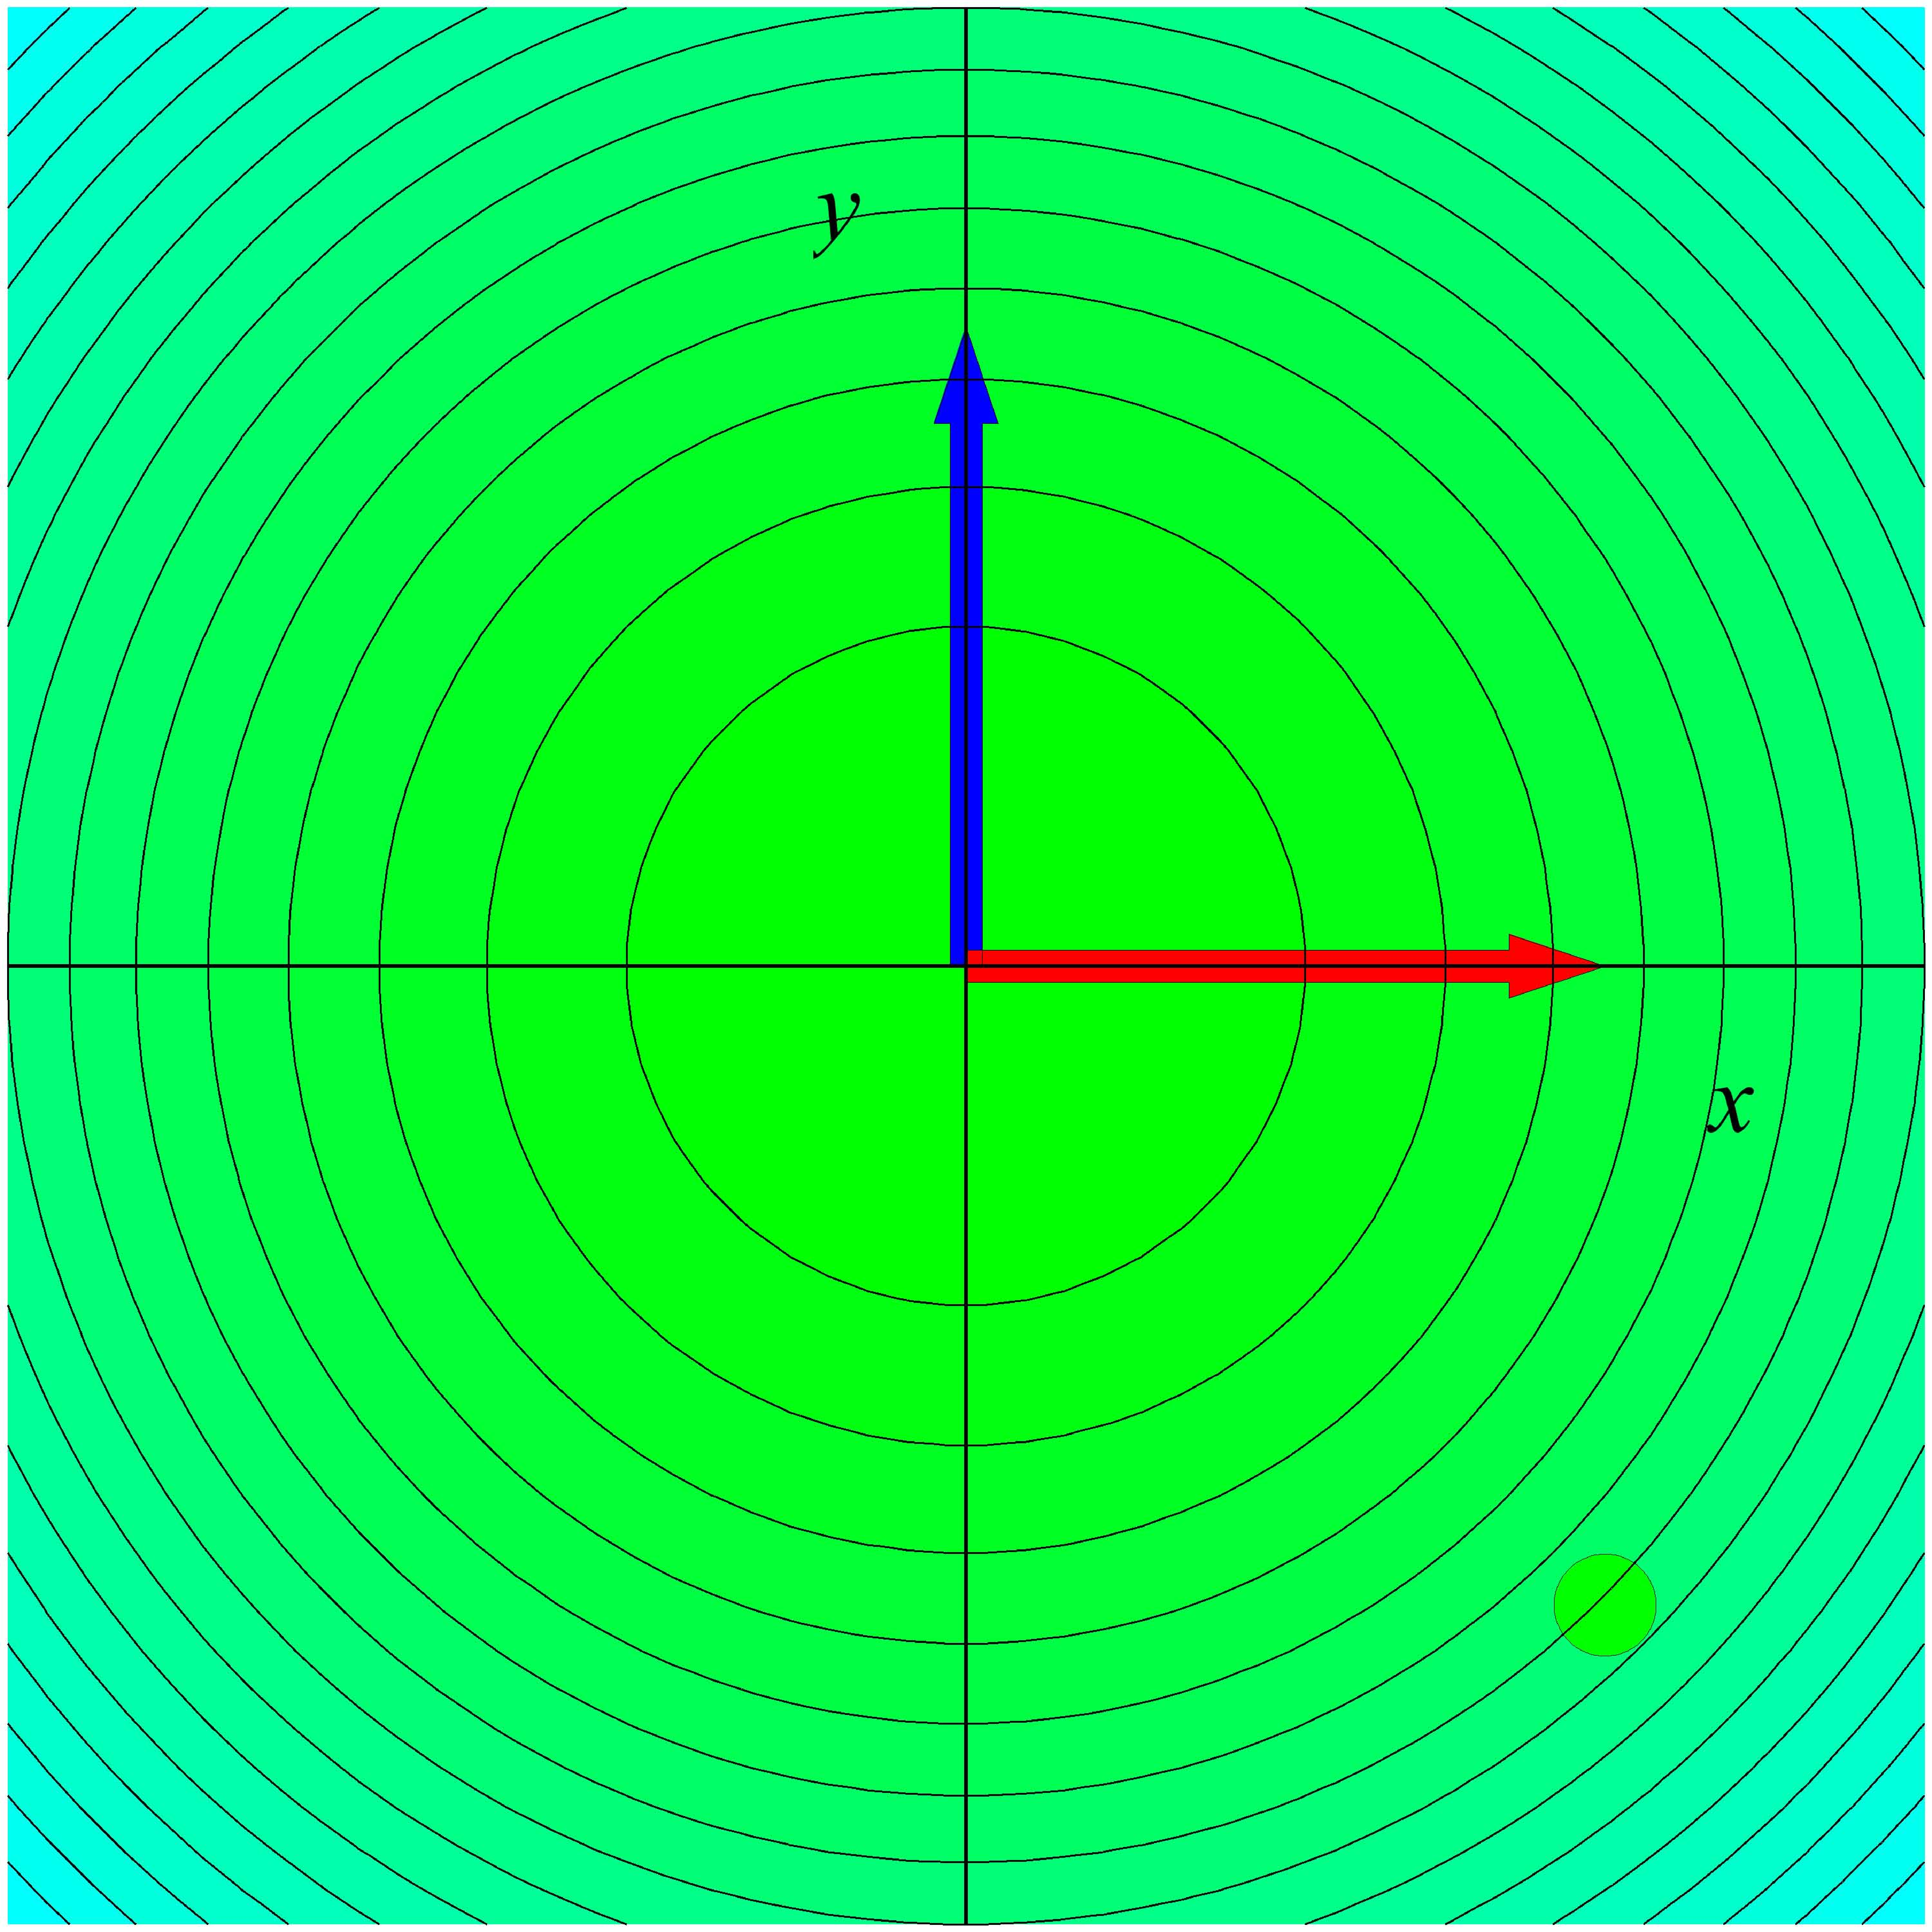
\includegraphics[height=25mm]{plotParabNiveau.pdf} \quad 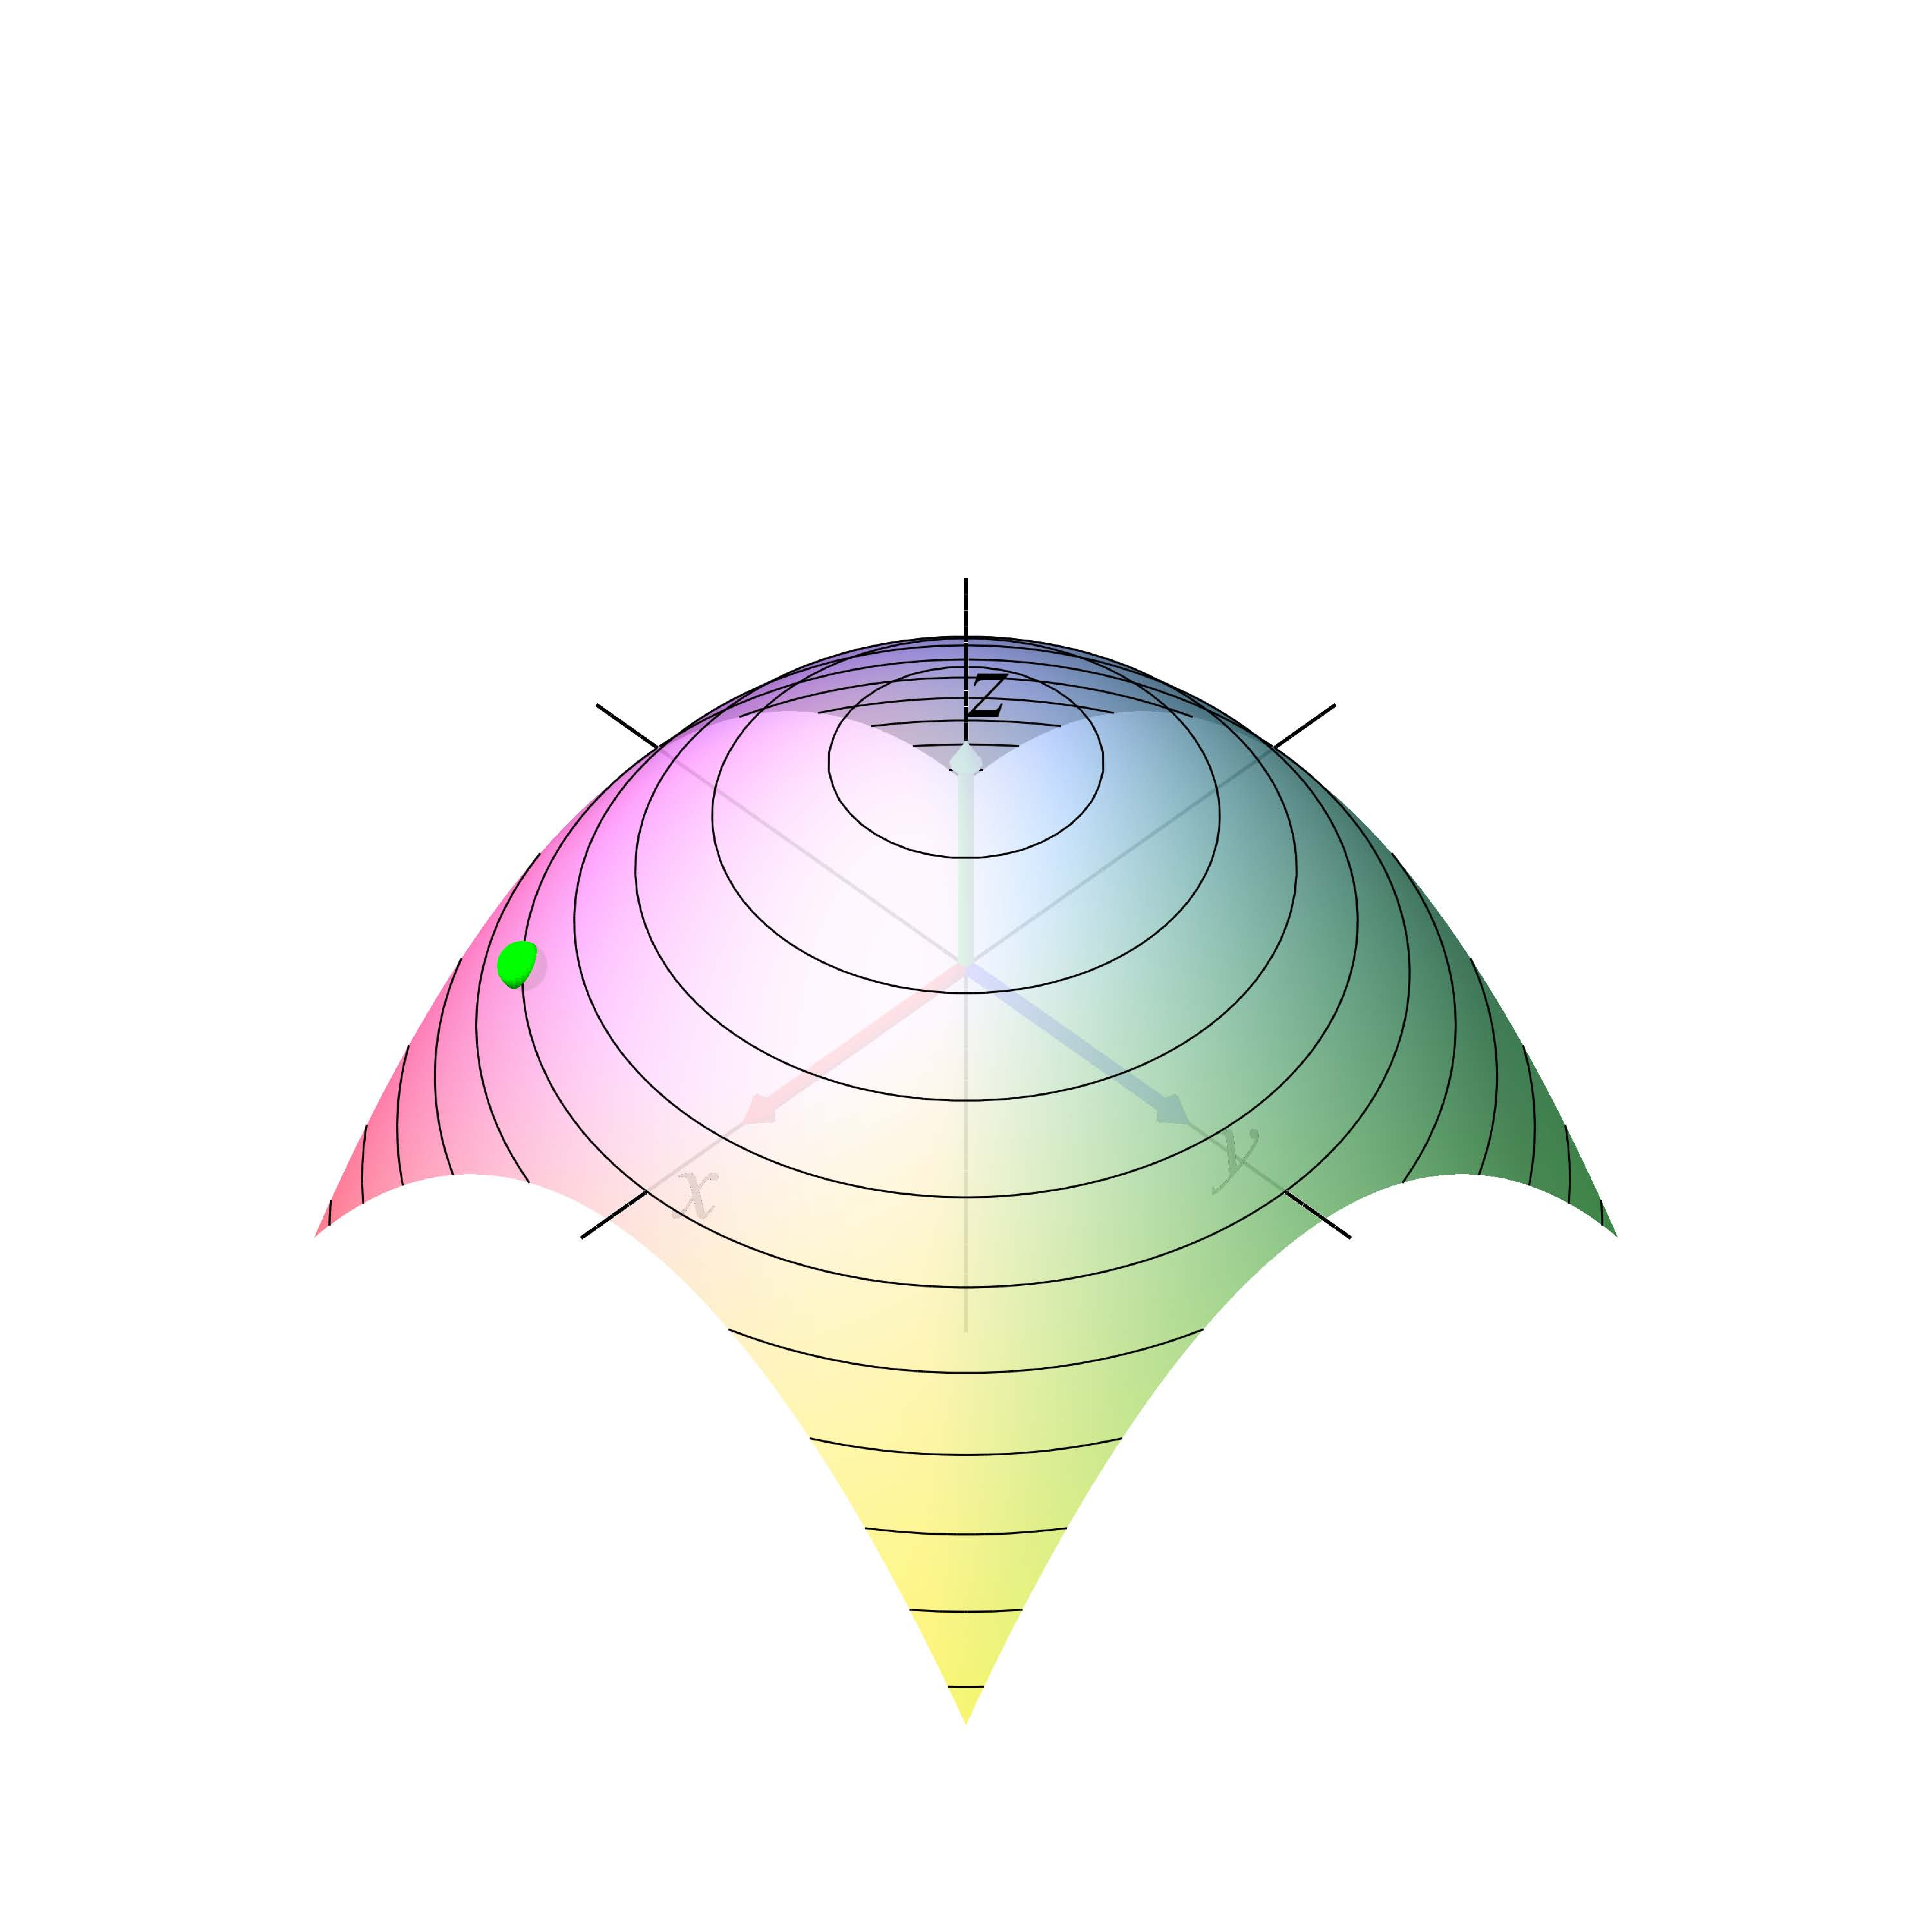
\includegraphics[height=80mm]{plotParabNiveauUP.pdf}}
\begin{center}
\caption{Grafen i $(x,y,z)$-rummet, niveaukurverne i $(x,y)$-planen, og højdesnitkurverne for funktionen $f(x,y) = 1- \frac{1}{2}\left(x^{2} + y^{2} \right)$.} \label{figParab}
\end{center}
\end{figure}


\begin{figure}[h]
\centerline{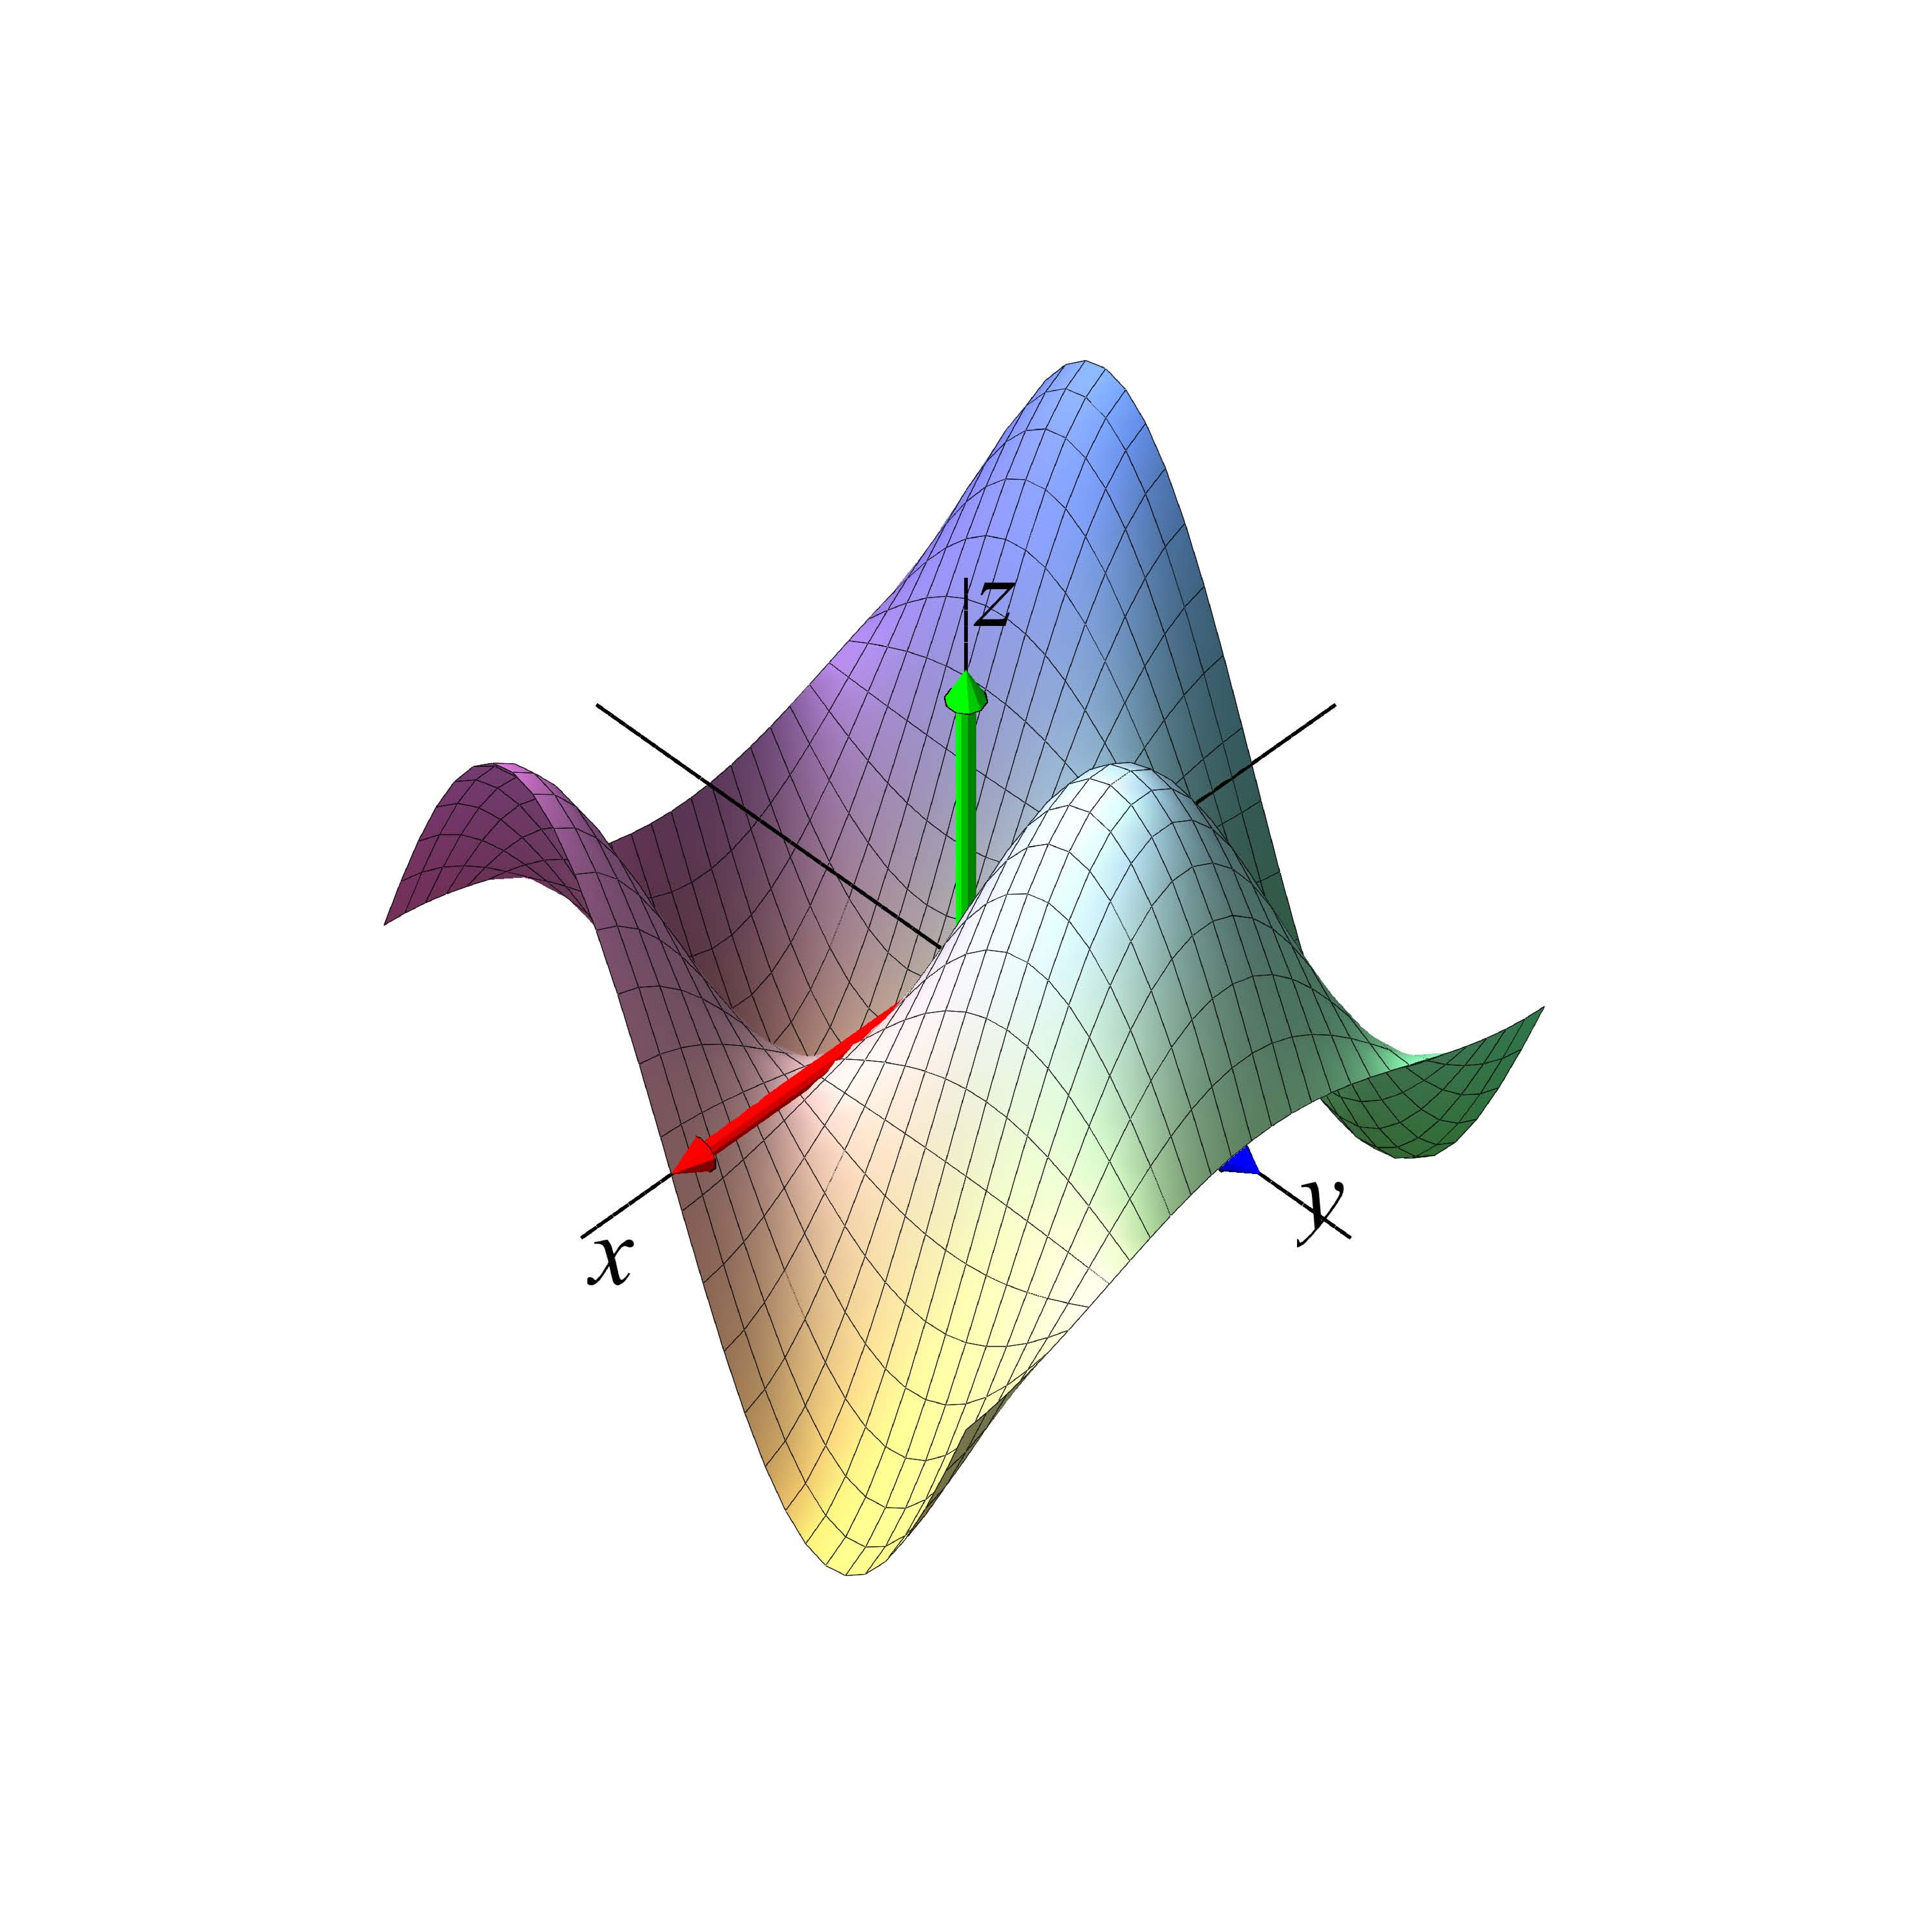
\includegraphics[height=80mm]{plotCosSin.pdf}\quad 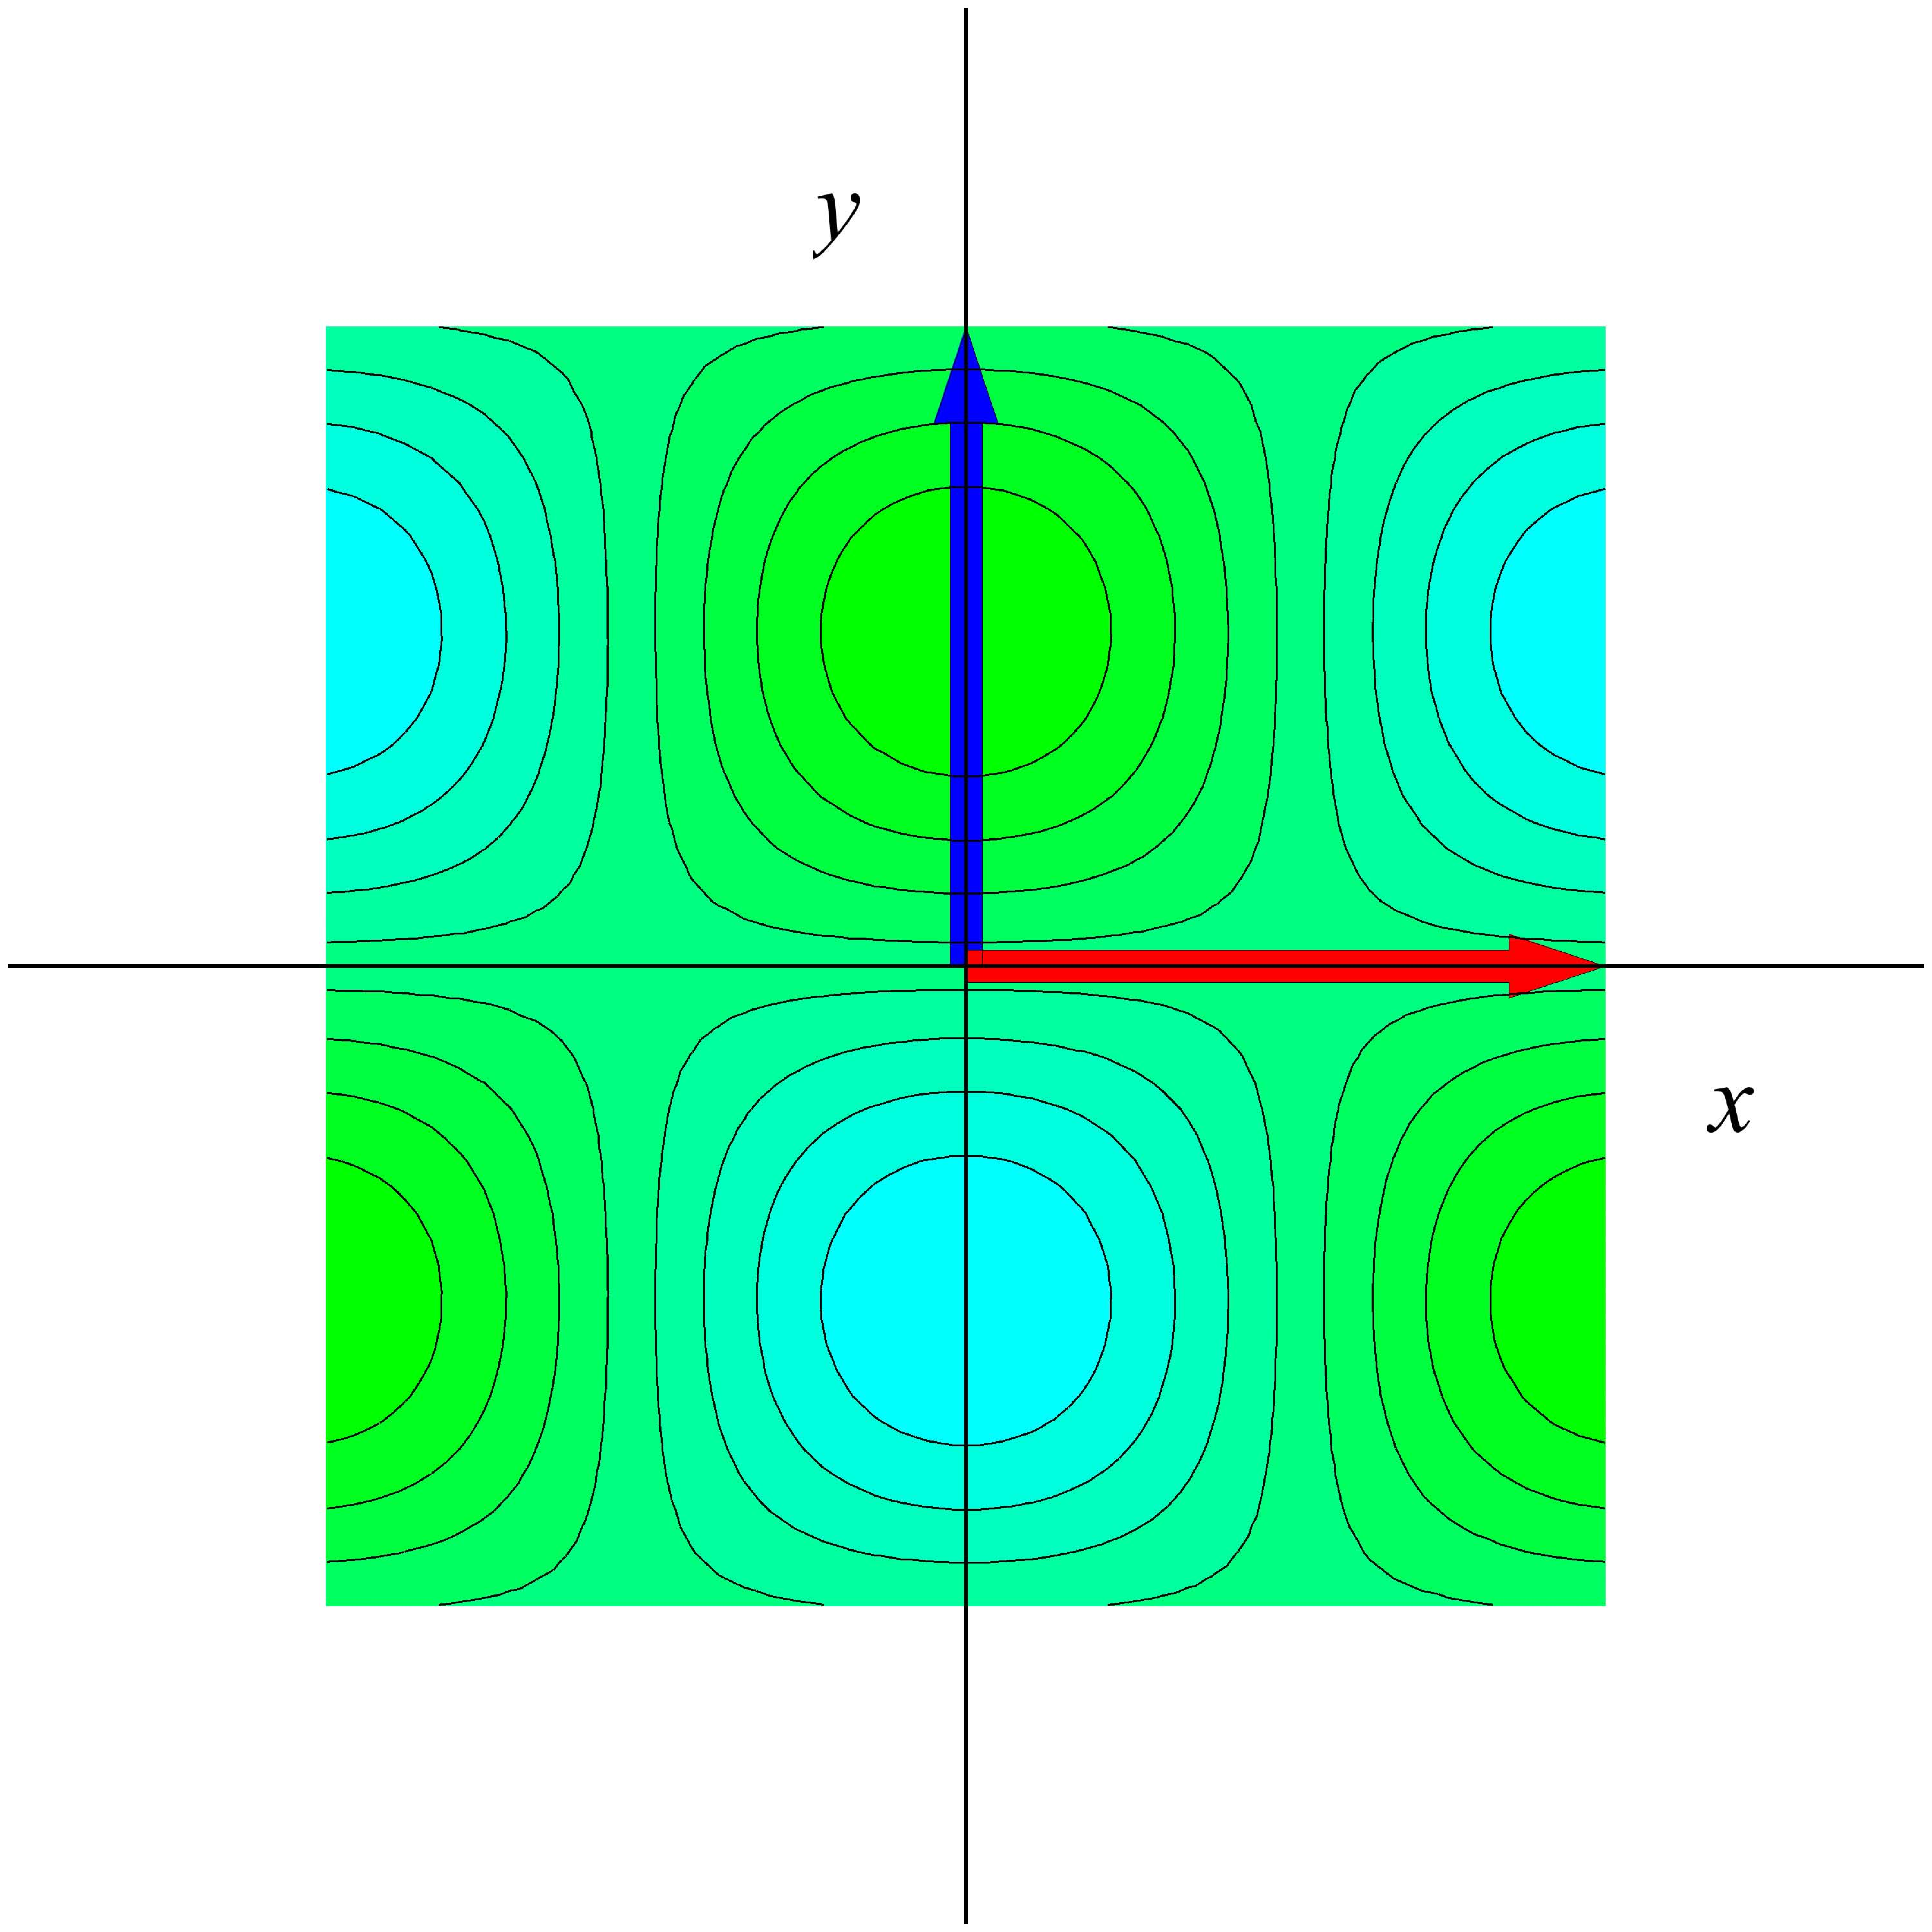
\includegraphics[height=25mm]{plotCosSinNiveau.pdf} \quad 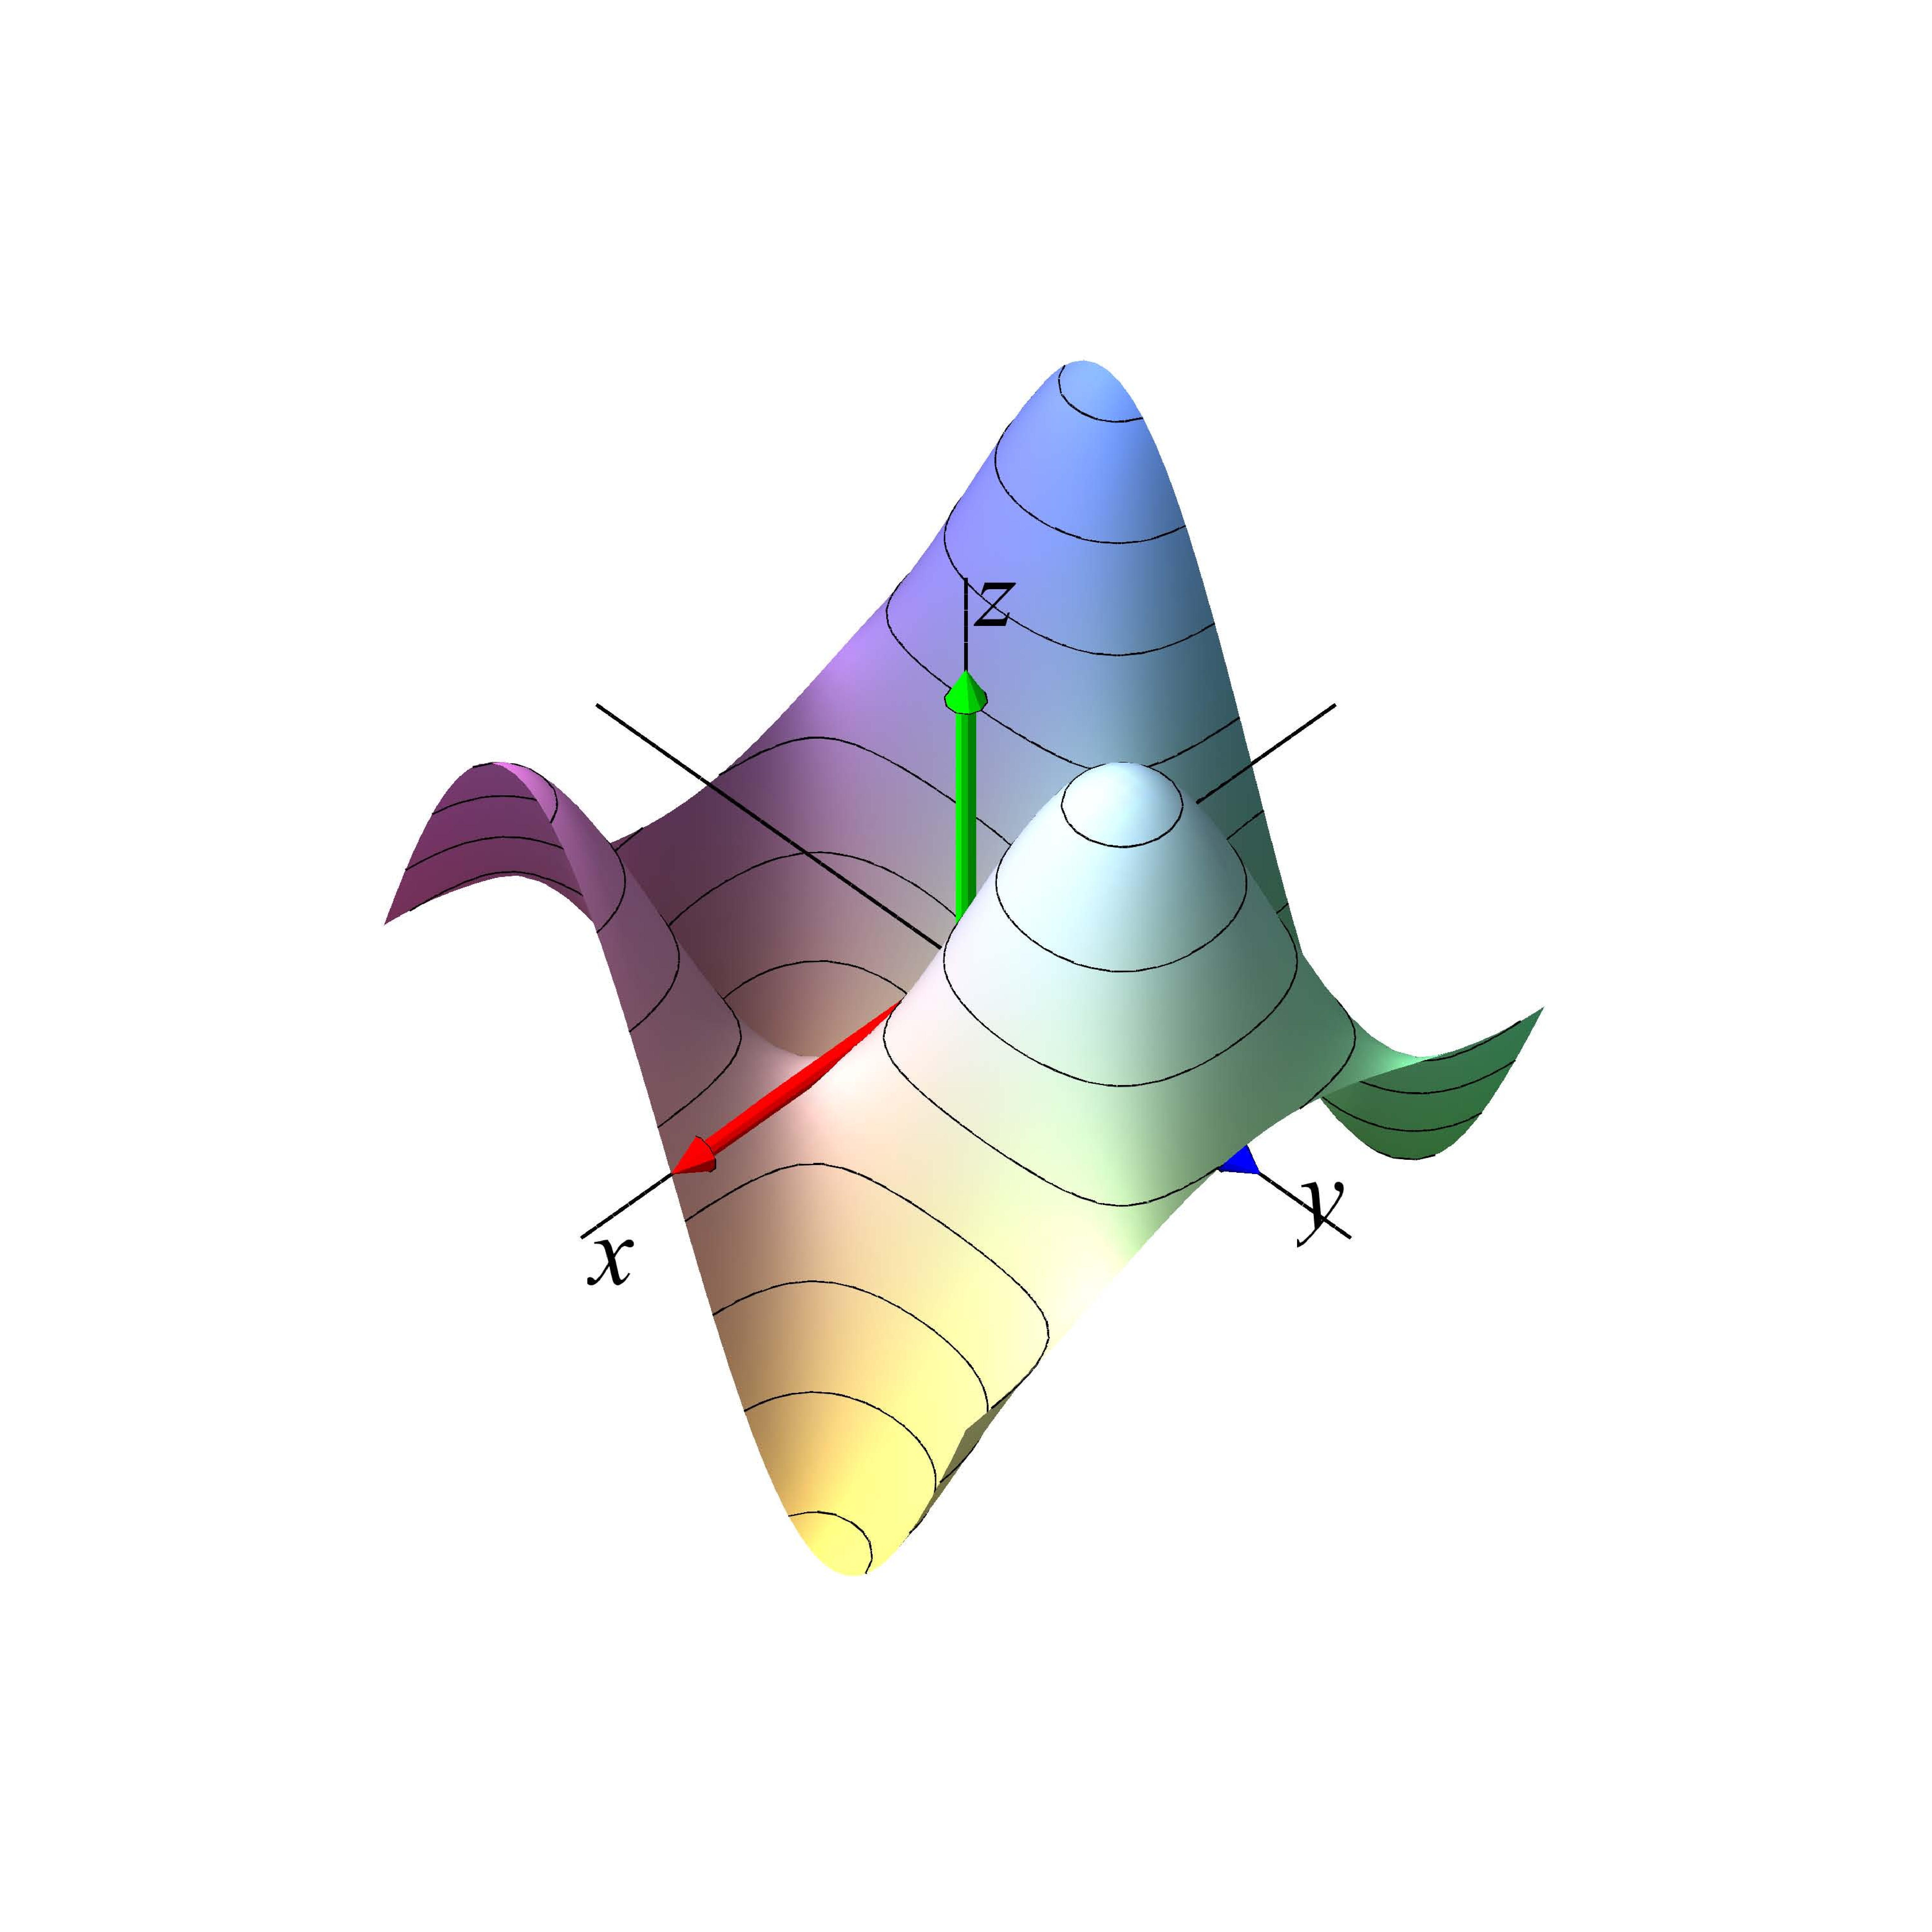
\includegraphics[height=80mm]{plotCosSinNiveauUP.pdf}}
\begin{center}
\caption{Grafen i $(x,y,z)$-rummet, niveaukurverne i $(x,y)$-planen, og højdesnitkurverne for funktionen $f(x,y) = \cos(3x)\cdot\sin(3y)$.} \label{figCosSin}
\end{center}
\end{figure}


%%%%%%%%%%%%%%%%%%%%%%%%%%%%%%%%%%%%%%%%%%%%%%%%%%%
%%%%%%%%%%%%%%%%%%%%%%%%%%%%%%%%%%%%%%%%%%%%%%%%%%%
%%%%%%%%%%%%%%%%%%%%%%%%%%%%%%%%%%%%%%%%%%%%%%%%%%%
%%%%%%%%%%%%%%%%%%%%%%%%%%%%%%%%%%%%%%%%%%%%%%%%%%%

\section{Epsilon-funktioner af to variable} \label{Epsilon}

En meget vigtig klasse af  funktioner af to variable er afstandsfunktionerne. For ethvert punkt $(x_{0}, y_{0})$ i planen definerer vi afstanden til $(x_{0}, y_{0})$ på velkendt måde:

\begin{definition}[Afstandsfunktioner]
Afstanden fra et punkt $(x,y)$ til et punkt $(x_{0}, y_{0})$ i $(x,y)$-planen
betegnes med
\begin{equation}
\rho_{(x_{0}, y_{0})}(x,y) = \sqrt{(x-x_{0})^{2} + (y-y_{0})^{2}} \quad.
\end{equation}
Dette er den sædvanlige afstand mellem de to punkter $(x,y)$ og $(x_{0}, y_{0})$ i planen --
bestemt med Pythagoras' sætning.
\end{definition}

\begin{aha}
Det er denne funktion vi vil bruge på samme måde som vi benyttede funktionen  $(x-x_{0})$ til definitionerne af
epsilon-funktioner af \'{e}n variabel og til definition af kontinuitet og differerentiabilitet af funktioner af \'{e}n variabel.
Læg mærke til, at $\rho_{(x_{0}, y_{0})}(x,y)$ altid er positiv eller $0$; og læg mærke til at værdien $0$ dog kun optræder for $(x, y) = (x_{0}, y_{0})$.
Funktionen $\rho_{(0,0)}(x,y)$, altså afstanden fra $(x,y)$ til $(x_{0}, y_{0}) = (0,0)$, er vist i figur \ref{figDist}. Læg mærke til, at niveaukurverne er ækvidistante, og at grafen er 'konisk spids' i kontaktpunktet til $(x,y)$-planen!
\end{aha}

\begin{figure}[h]
\centerline{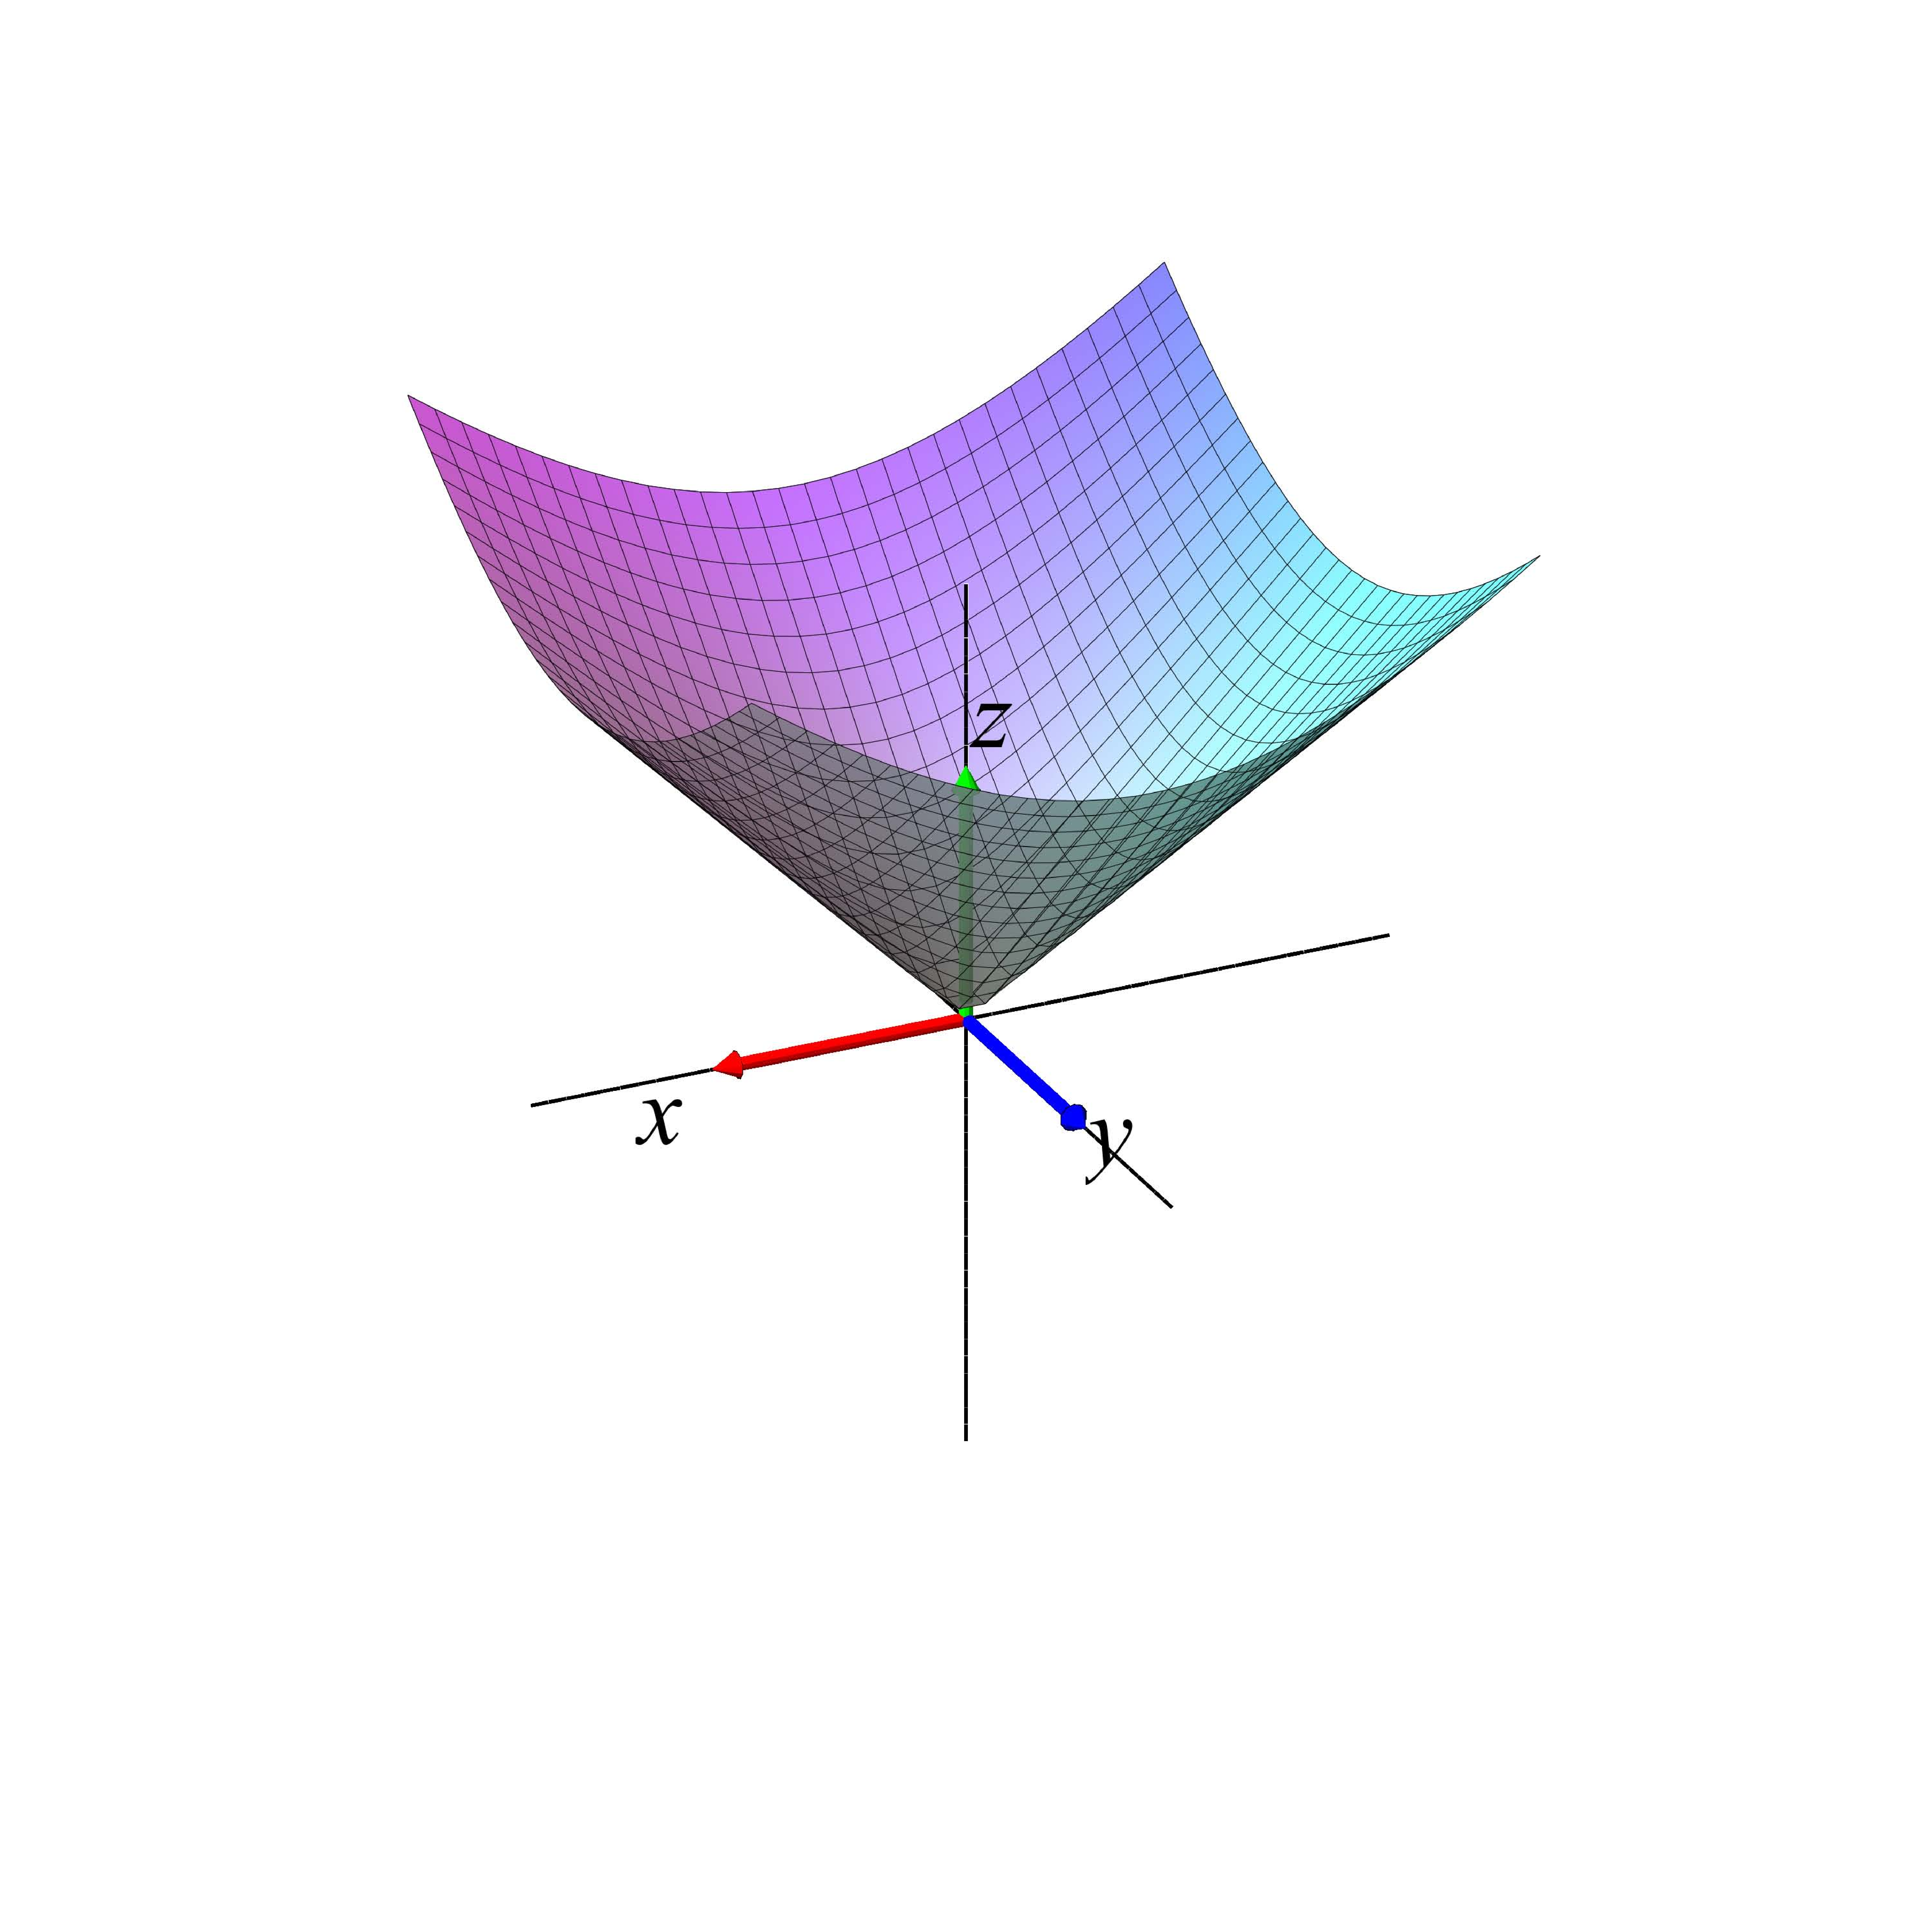
\includegraphics[height=80mm]{plotDist.pdf}\quad 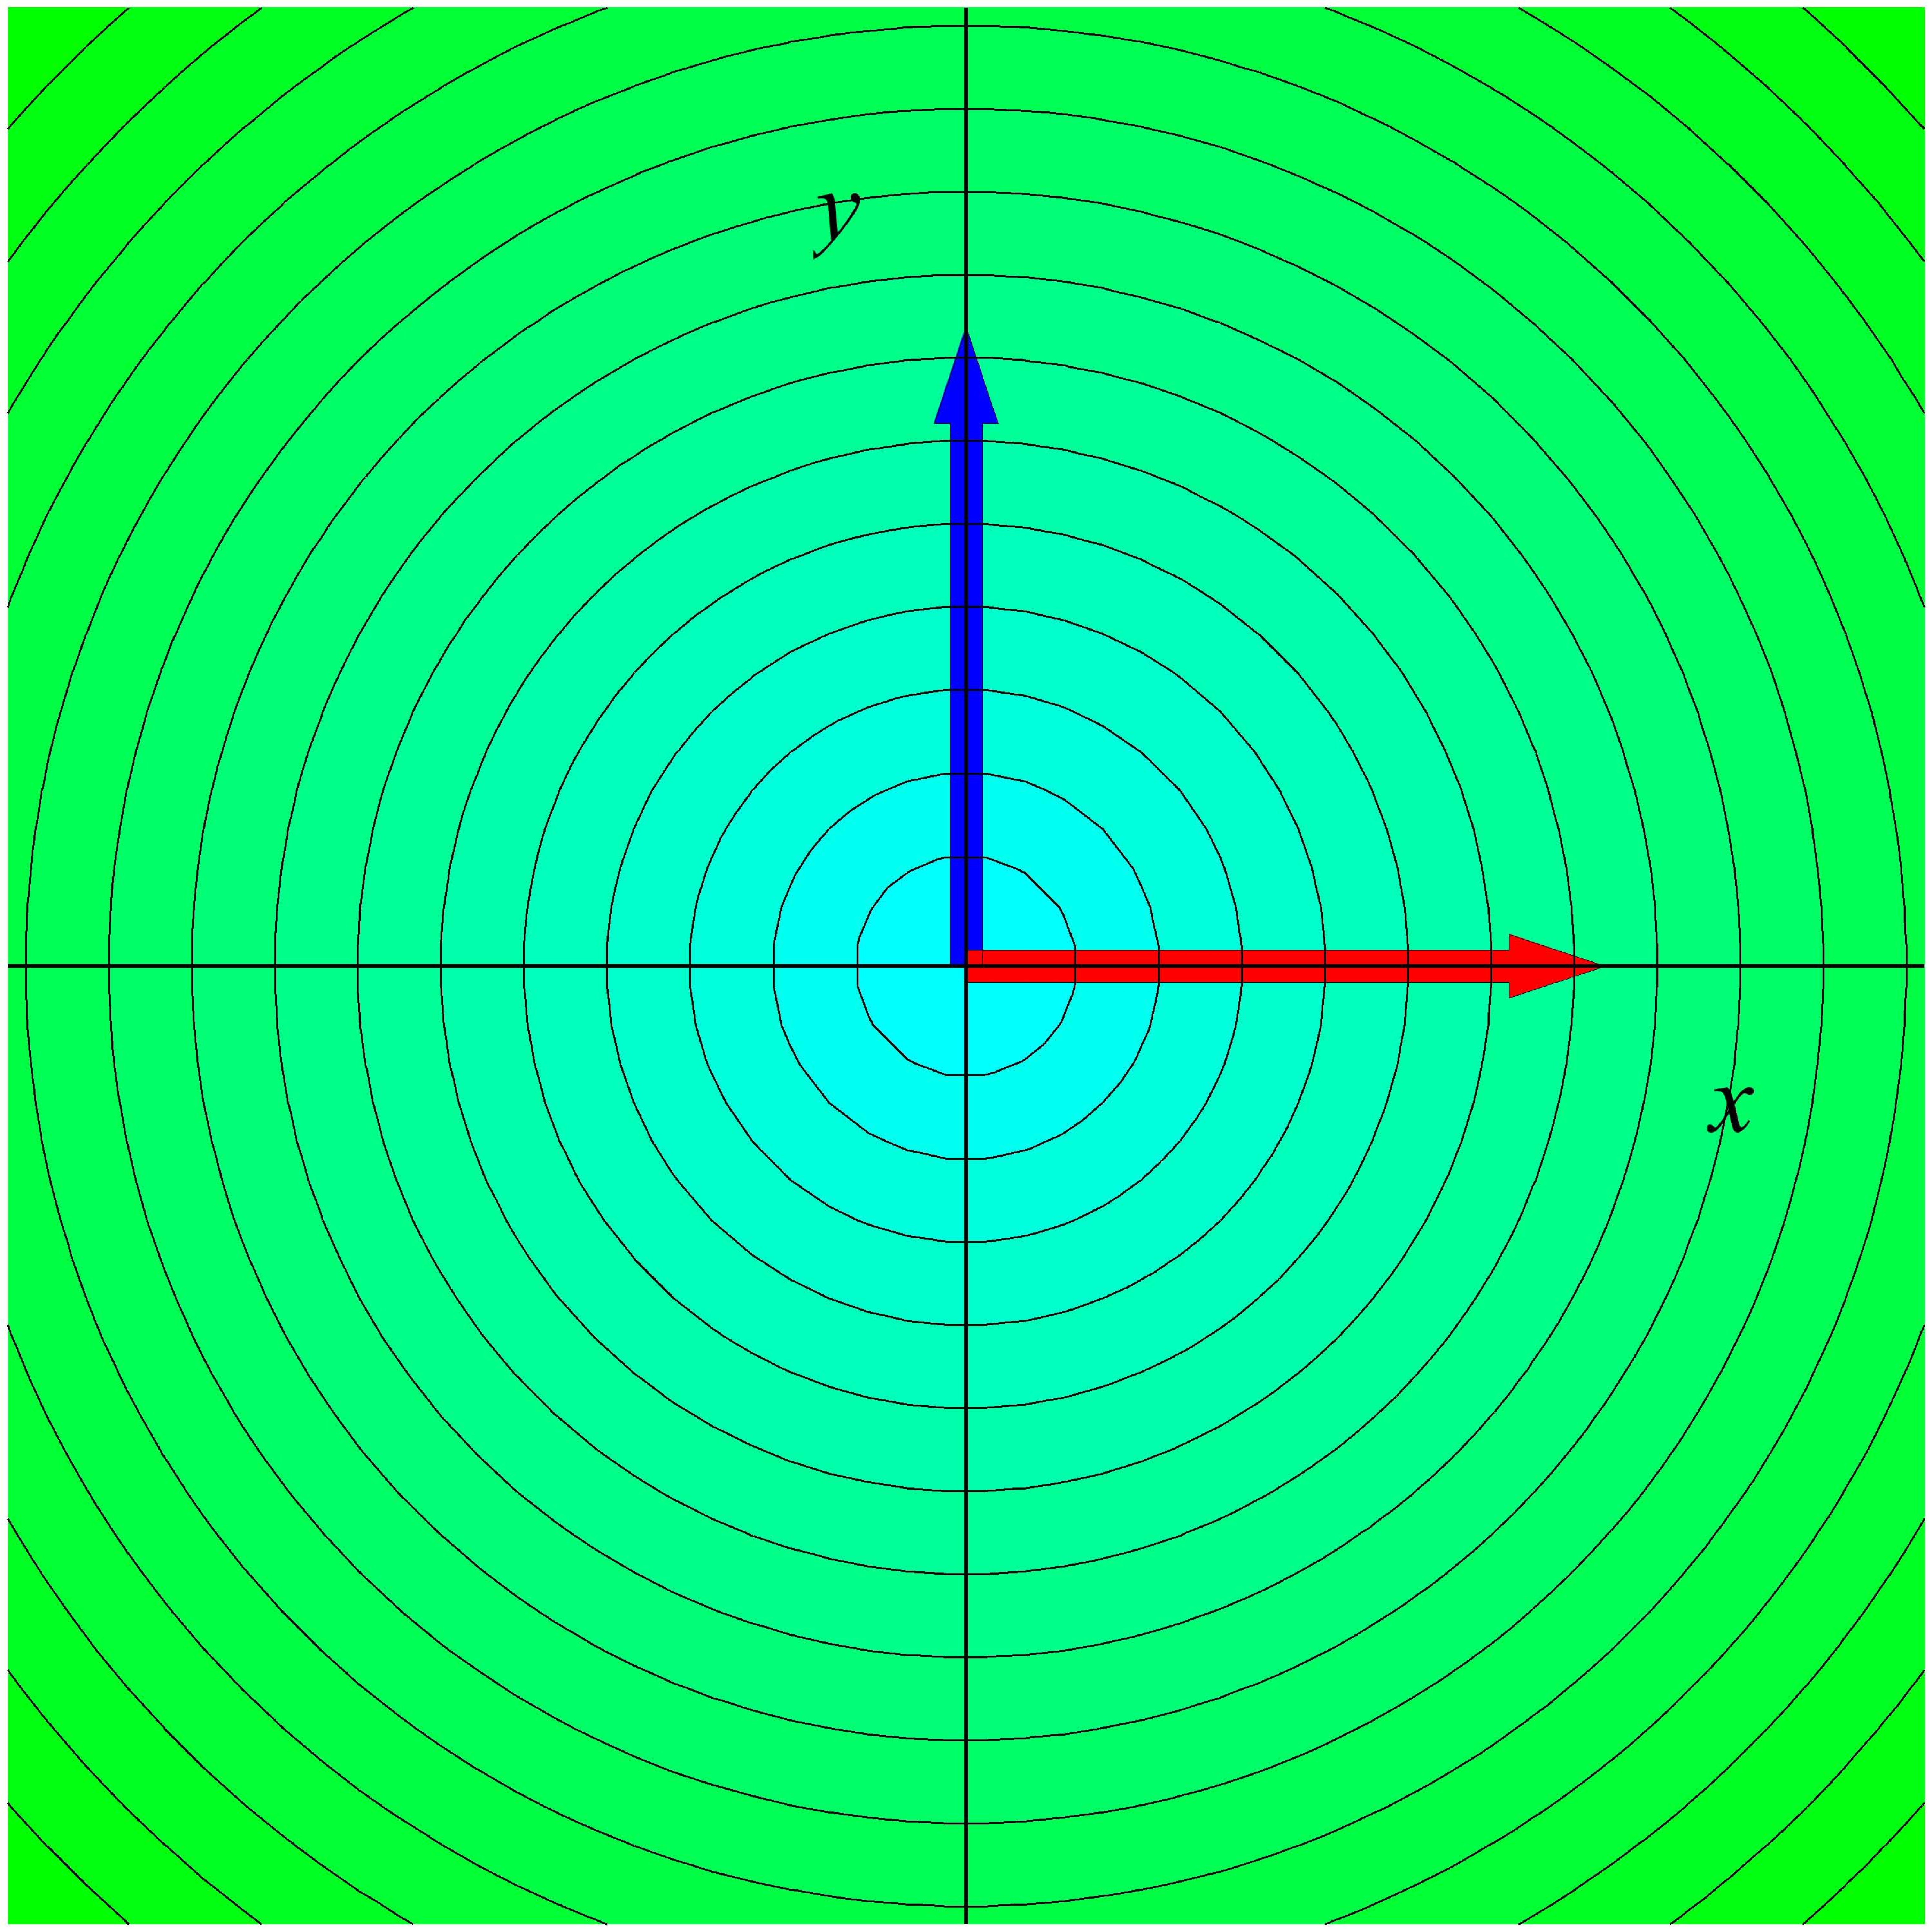
\includegraphics[height=25mm]{plotDistNiveau.pdf} \quad 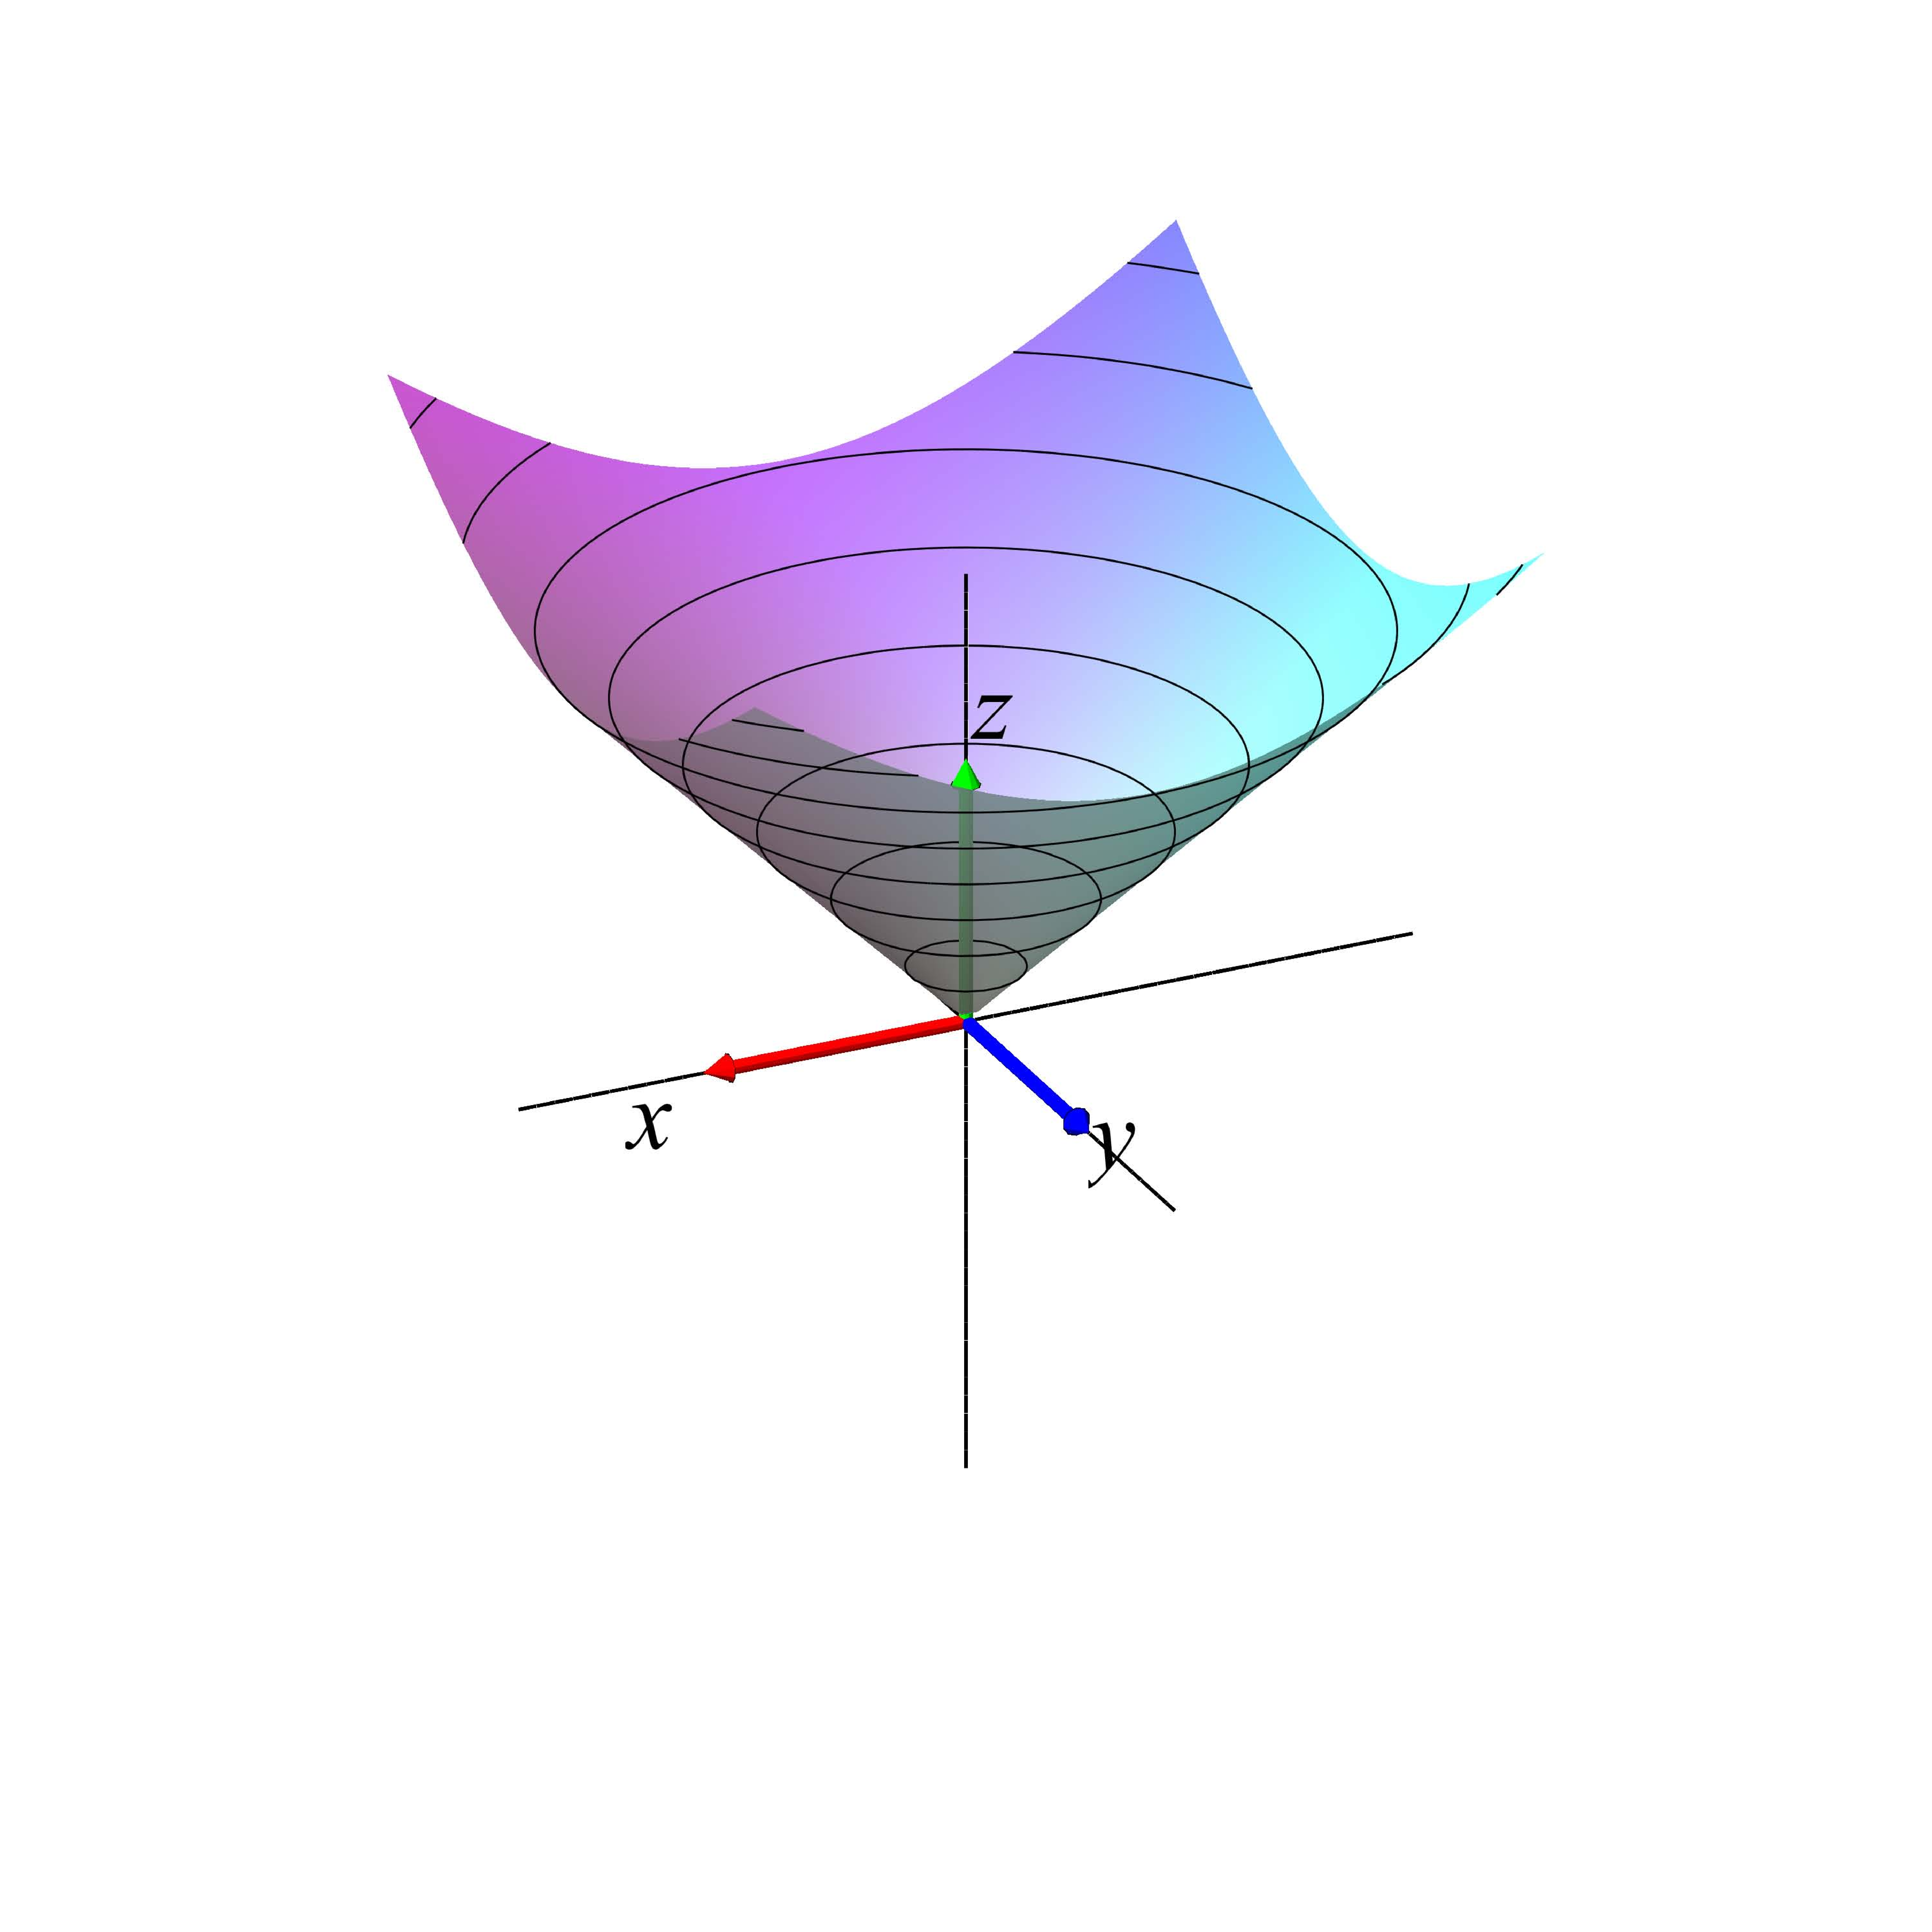
\includegraphics[height=80mm]{plotDistNiveauUP.pdf}}
\begin{center}
\caption{Grafen for afstandsfunktionen  $\rho_{(0,0)}(x,y)$ til punktet $(x_{0}, y_{0}) = (0,0)$, funktionens niveaukurver, og højdesnit-kurverne på grafen.} \label{figDist}
\end{center}
\end{figure}


Vi er nu klar til at definere klassen af epsilonfunktioner af to variable:

\begin{definition}[Epsilonfunktioner af to variable]
Enhver funktion $\varepsilon(x,y)$ som er defineret i et åbent område i $\mathbb{R}^{2}$ indeholdende $(0,0)$, og som antager værdien $0$ i $(x,y) = (0,0)$, og som derudover går imod $0$ når $(x,y)$ går imod $(x_{0}, y_{0})$ kaldes en \ind{epsilon-funktion af $(x,y)$}{epsilon-funktion af $(x,y)$}. Epsilon-funktioner af to variable er altså karakteriserede ved egenskaberne:
\begin{equation}
\varepsilon(0,0) = 0 \quad  \textrm{og} \quad \varepsilon(x,y) \to 0 \quad \textrm{for} \quad (x,y) \to (0,0) \quad .
\end{equation}
Den sidste betingelse betyder, at den numeriske værdi af funktionsværdierne $\varepsilon(x,y)$ kan gøres så lille som ønsket ved blot at vælge $(x,y)$ \emph{tilstrækkelig tæt på} $(0,0)$. Helt præcis betyder betingelsen: For ethvert helt positivt tal $k$ findes der et helt positivt tal $K$ sådan at $|\varepsilon(x,y)| < 1/k$ for alle $(x,y)$ med $\rho_{(x_{0}, y_{0})}(x,y) < 1/K\,$.
\end{definition}


\begin{aha}
Det følger direkte af definitionen, at afstandsfunktionen $\rho_{(x_{0}, y_{0})}(x,y)$ til et punkt $(x_{0}, y_{0})$ selv er en epsilonfunktion af $x-x_{0}$ og $y-y_{0}$.
\end{aha}

%%%%%%%%%%%%%%%%%%%%%%%%%%%%%%%%%%%%%%%%%%%%%%%%%%%
%%%%%%%%%%%%%%%%%%%%%%%%%%%%%%%%%%%%%%%%%%%%%%%%%%%
%%%%%%%%%%%%%%%%%%%%%%%%%%%%%%%%%%%%%%%%%%%%%%%%%%%

\section{Kontinuerte funktioner af to variable} \label{Epsilon}
Som for funktioner af \'{e}n variabel definerer vi kontinuitet for funktioner af to variable ved hjælp af klassen af epsilonfunktioner:

\begin{definition}[Kontinuerte funktioner af to variable] \label{defKont2var}
En funktion $f(x,y)$ er kontinuert i $(x_{0}, y_{0})$ hvis der eksisterer en epsilon-funktion $\varepsilon_{f}(x-x_{0}, y-y_{0})$ sådan at følgende gælder i et åbent område der indeholder $(x_{0}, y_{0})$:
\begin{equation}
f(x,y) = f(x_{0}, y_{0}) + \varepsilon_{f}(x-x_{0}, y-y_{0}) \quad.
\end{equation}
Hvis $f(x,y)$ er kontinuert i alle $(x_{0}, y_{0})$ i et givet åbent område i $\mathcal{D}m(f)$, så siger vi, at $f(x,y)$ er kontinuert i hele området.
\end{definition}


Enhver epsilonfunktion af  $x-x_{0}$ og $y-y_{0}$ som f.eks. $\rho_{(x_{0}, y_{0})}(x,y)$ er derfor kontinuert i $(x_{0}, y_{0})$.
Grafer og niveaukurver kan ofte afsløre, om en funktion er kontinuert i et punkt.

\begin{theorem}[Inspektion af niveau-mængder] \label{thmInspektionNiveau}
Hvis en funktion $f(x,y)$ har to niveau-mængder $\mathcal{K}_{c_{1}}$ og $\mathcal{K}_{c_{2}}$ (hvor $c_{1} \neq c_{2}$) som begge indeholder punkter $(x,y)$ vilkårligt tæt på $(x_{0}, y_{0})$, så er $f(x,y)$ ikke kontinuert i $(x_{0}, y_{0})$.
\end{theorem}
\begin{bevis}
Antag, at $f(x,y)$ er kontinuert i $(x_{0}, y_{0})$. Hvis vi går i mængden  $\mathcal{K}_{c_{1}}$ hen mod $(x_{0}, y_{0})$ så skal (pr. kontinuitet) $f(x_{0}, y_{0})$ være $c_{1}$. Hvis vi derimod går i mængden  $\mathcal{K}_{c_{2}}$ hen mod $(x_{0}, y_{0})$ får vi $f(x_{0}, y_{0}) = c_{2}$, hvilket er en modstrid, da $c_{1} \neq c_{2}$.
\end{bevis}

\begin{aha}
To niveaukurver hørende til forskellige funktionsværdier for en funktion $f(x,y)$ kan ligge meget tæt på hinanden i $(x, y)$-planen -- men altså ikke vilkårligt tæt -- hvis funktionen er kontinuert.
\end{aha}

\begin{example}[En funktion som ikke er kontinuert]\label{exampDiskont}
Vi ser på $0$-udvidelsen $\widehat{f}(x,y)$ af funktionen
\begin{equation}
f(x,y) = \frac{x^{2}\,y}{x^{4} + y^{2}} \quad , \quad \textrm{hvor} \quad (x,y) \in \mathbb{R}^{2} \setminus \{\,(0,0) \,\} \quad.
\end{equation}
Det vil sige:
\begin{equation}
\widehat{f}(x,y) = \left\{
           \begin{array}{ll}
             \frac{x^{2}\,y}{x^{4} + y^{2}} & \hbox{\,\,for $(x,y) \neq (0,0)$} \\
             0 & \hbox{\,\,for $(x,y)= (0,0) $\quad . }
           \end{array}
         \right.
\end{equation}
Funktionen kan inspiceres i figur \ref{figDiskont}. Ved den inspektion bemærkes, at niveaukurverne 'ligner parabler' igennem $(0,0)$.
Vi vil teste den hypotese, at det faktisk er parabler: Hvis vi sætter $y = c\,x^{2}$ (parabelligning) får vi følgende udregninger:
\begin{equation}
\begin{aligned}
f(x,y) &= f(x, c\,x^{2})  \\
&= \frac{x^{2}\,c\,x^{2}}{x^{4} + (c\,x^{2})^{2}} \\
&= \frac{c\,x^{4}}{(1 + c^{2})\,x^{4} } \\
&= \frac{c}{1 + c^{2}} \quad,
\end{aligned}
\end{equation}
hvilket netop betyder, at parablerne $y = c\,x^{2}$ er (indeholdt i) niveau-mængden $\mathcal{K}_{c/(1 + c^{2})}$. Da alle parablerne går igennem $(0,0)$ følger det af sætning \ref{thmInspektionNiveau} at funktionen $f(x,y)$ ikke er kontinuert i $(0,0)$.

\end{example}

\begin{figure}[h]
\centerline{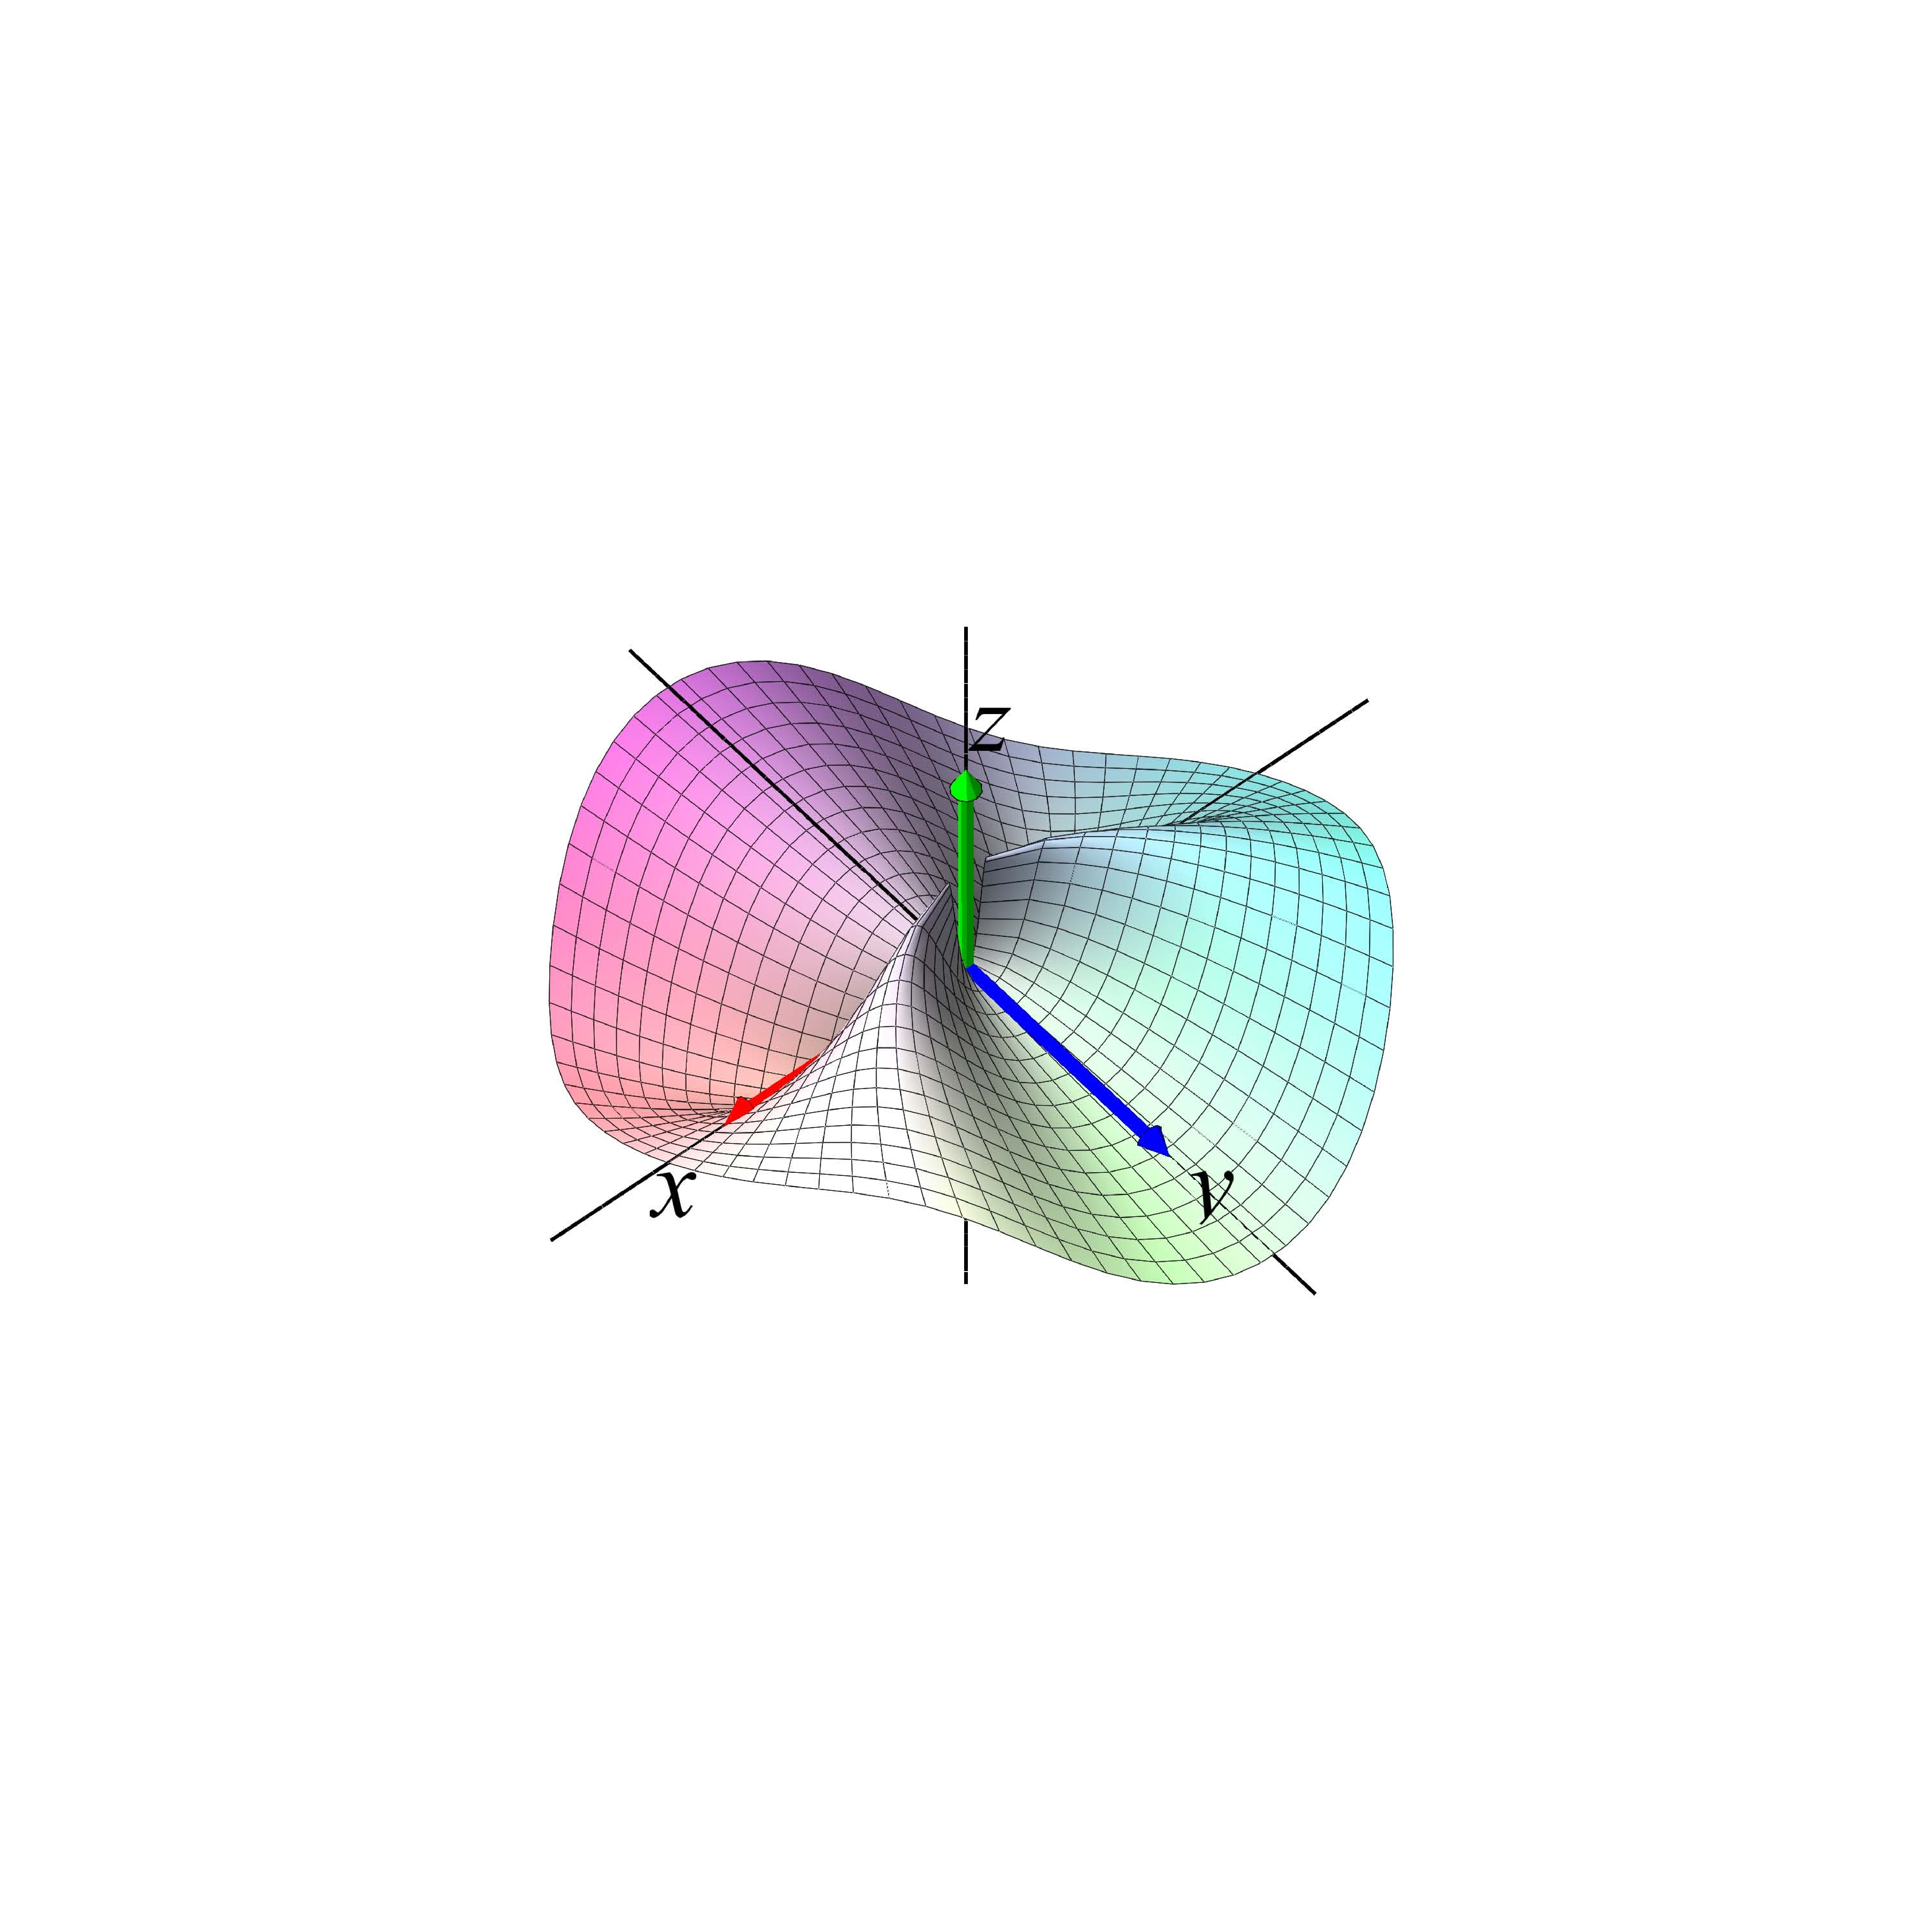
\includegraphics[height=90mm]{plotDiskontRes.pdf}\quad 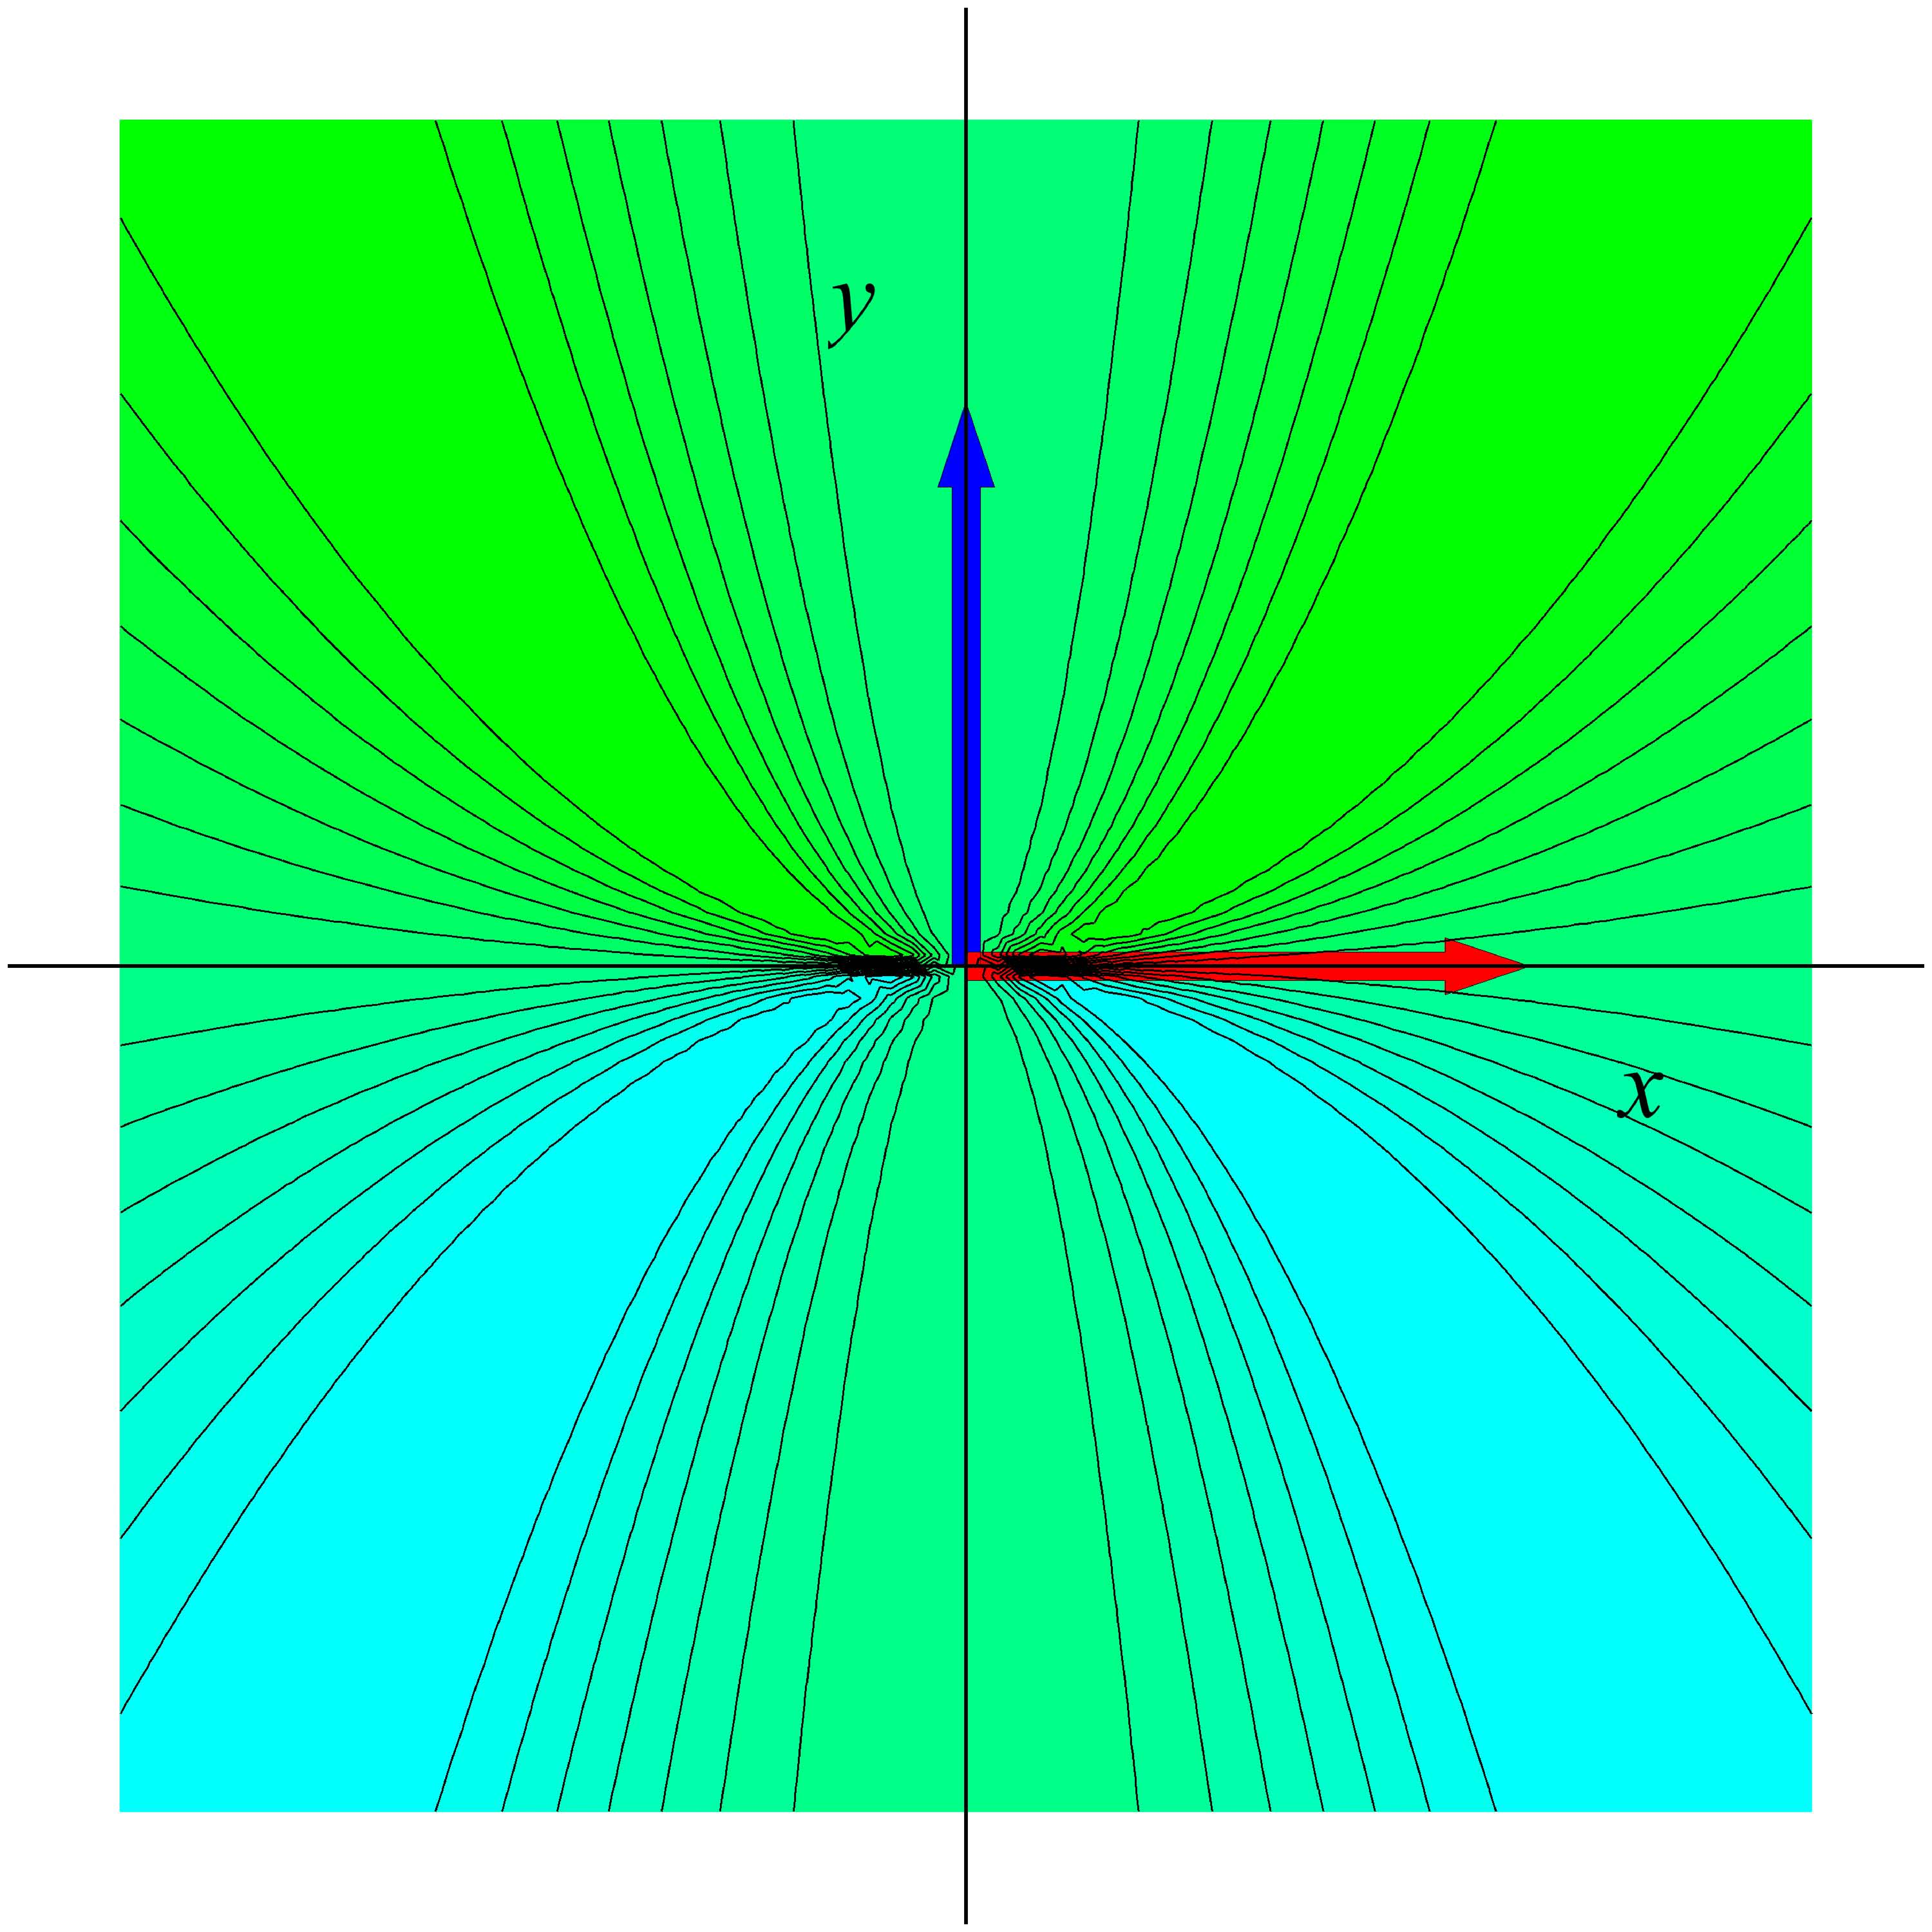
\includegraphics[height=35mm]{plotDiskontNiveau.pdf}}
\begin{center}
\caption{Grafen i rummet  og niveaukurve-forløbet i planen for funktionen i eksempel \ref{exampDiskont}.} \label{figDiskont}
\end{center}
\end{figure}

\begin{exercise}
Vis, at $0$-udvidelsen $\widehat{f}(x,y)$ af følgende funktion ikke er kontinuert i $(0,0)$:
\begin{equation}
f(x,y) = \frac{x}{x^{2} + y^{2}} \quad .
\end{equation}
\end{exercise}

\begin{example}[Første-grads-polynomier er kontinuerte]
Vi vil vise, at $f(x,y) = \alpha x + \beta y + \gamma$ er kontinuert i $(x_{0}, y_{0})$.
Det følger direkte af, at
\begin{equation}
f(x,y) - f(x_{0}, y_{0}) =  \alpha (x-x_{0}) + \beta (y-y_{0}) \to 0 \quad \textrm{for} \quad (x,y) \to (x_{0}, y_{0})) \quad,
\end{equation}
sådan at
\begin{equation}
f(x,y) = f(x_{0}, y_{0}) + \varepsilon_{f}(x-x_{0}, y-y_{0})
\end{equation}
med epsilonfunktionen $ \varepsilon_{f}(x-x_{0}, y-y_{0}) = \alpha (x-x_{0}) + \beta (y-y_{0})$. Overvej hvorfor dette er en epsilonfunktion.
\end{example}

\begin{exercise}
Vis, at følgende anden-grads polynomium er kontinuert i $(0,0)$:
\begin{equation}
f(x,y) = x^{2} + y^{2} \quad .
\end{equation}
\end{exercise}

\begin{exercise}
Vis, at $0$-udvidelsen af følgende funktion er kontinuert i $(0,0)$:
\begin{equation}
f(x,y) = \frac{x\,y^{2}}{x^{2} + y^{2}} \quad .
\end{equation}
\end{exercise}


\begin{example}[Kvadratroden af afstandsfunktionen]
Funktionen $f(x, y) = \sqrt{\rho_{(x_{0}, y_{0})}(x,y)}$ er -- ligesom $\rho_{(x_{0}, y_{0})}(x,y)$ selv -- en epsilonfunktion og er derfor kontinuert i $(x_{0}, y_{0})$. Se figur \ref{figSqrt}.
\end{example}

\begin{figure}[h]
\centerline{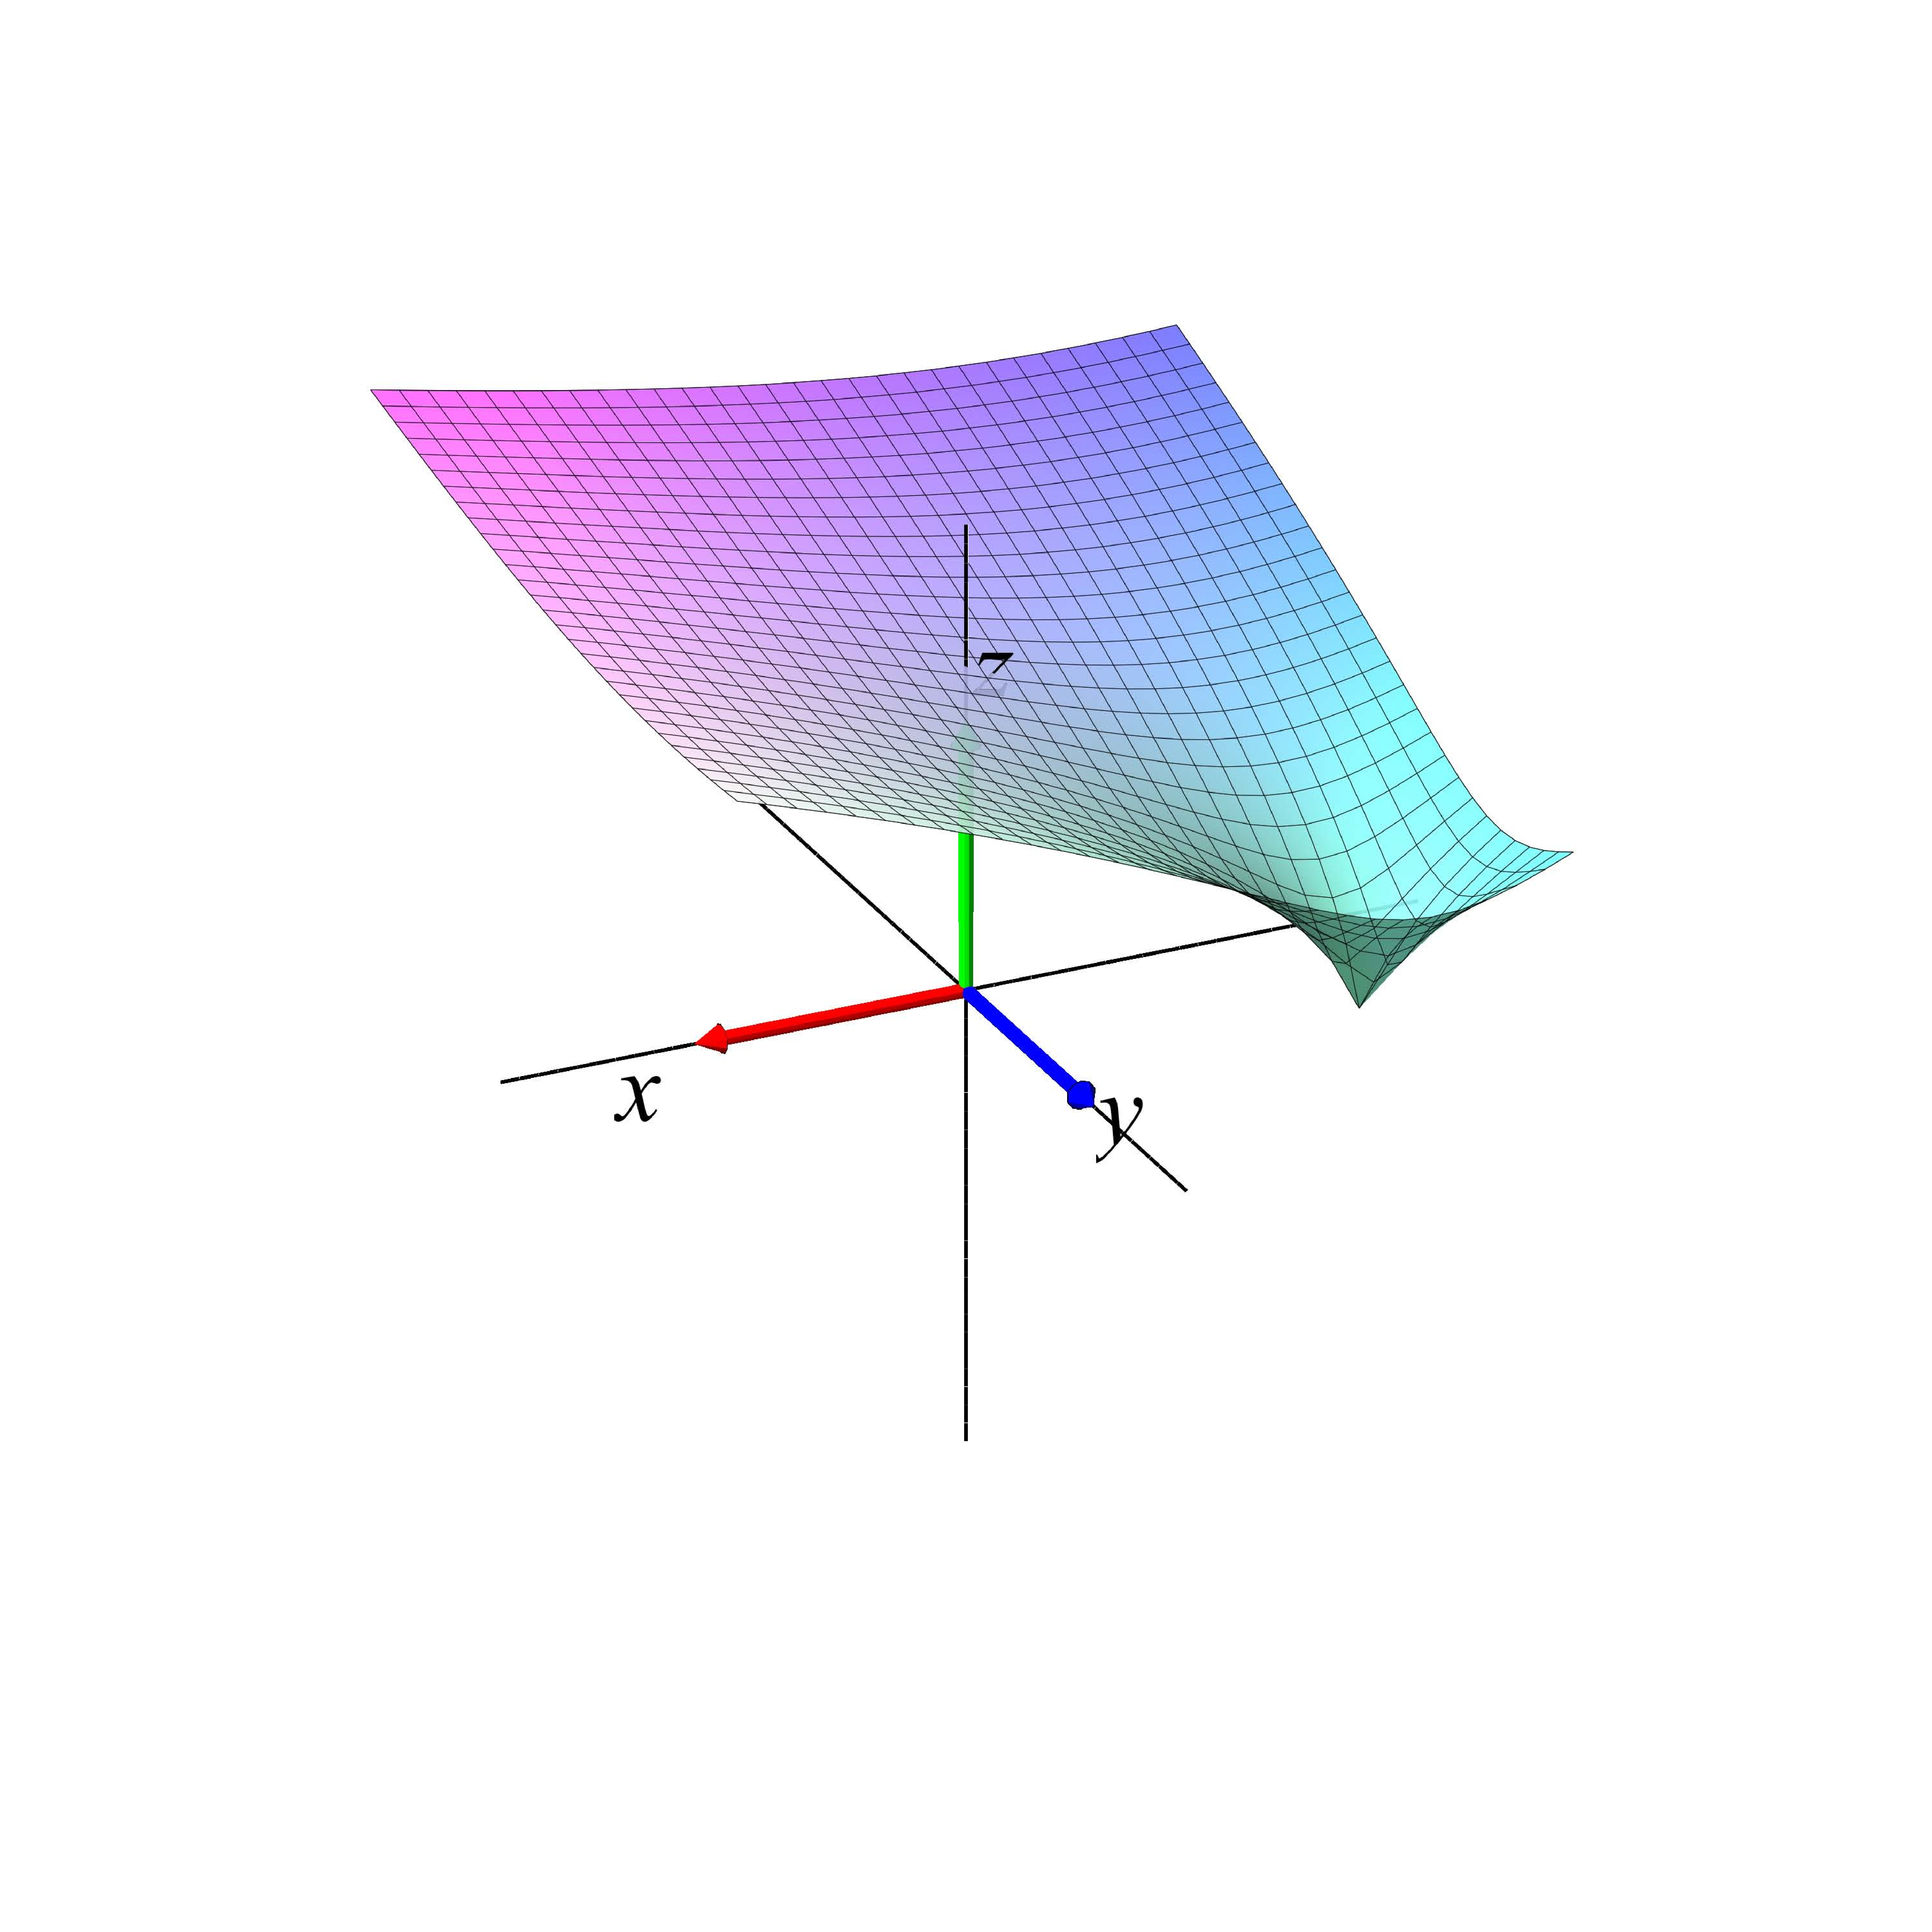
\includegraphics[height=80mm]{plotSqrt.pdf}\quad 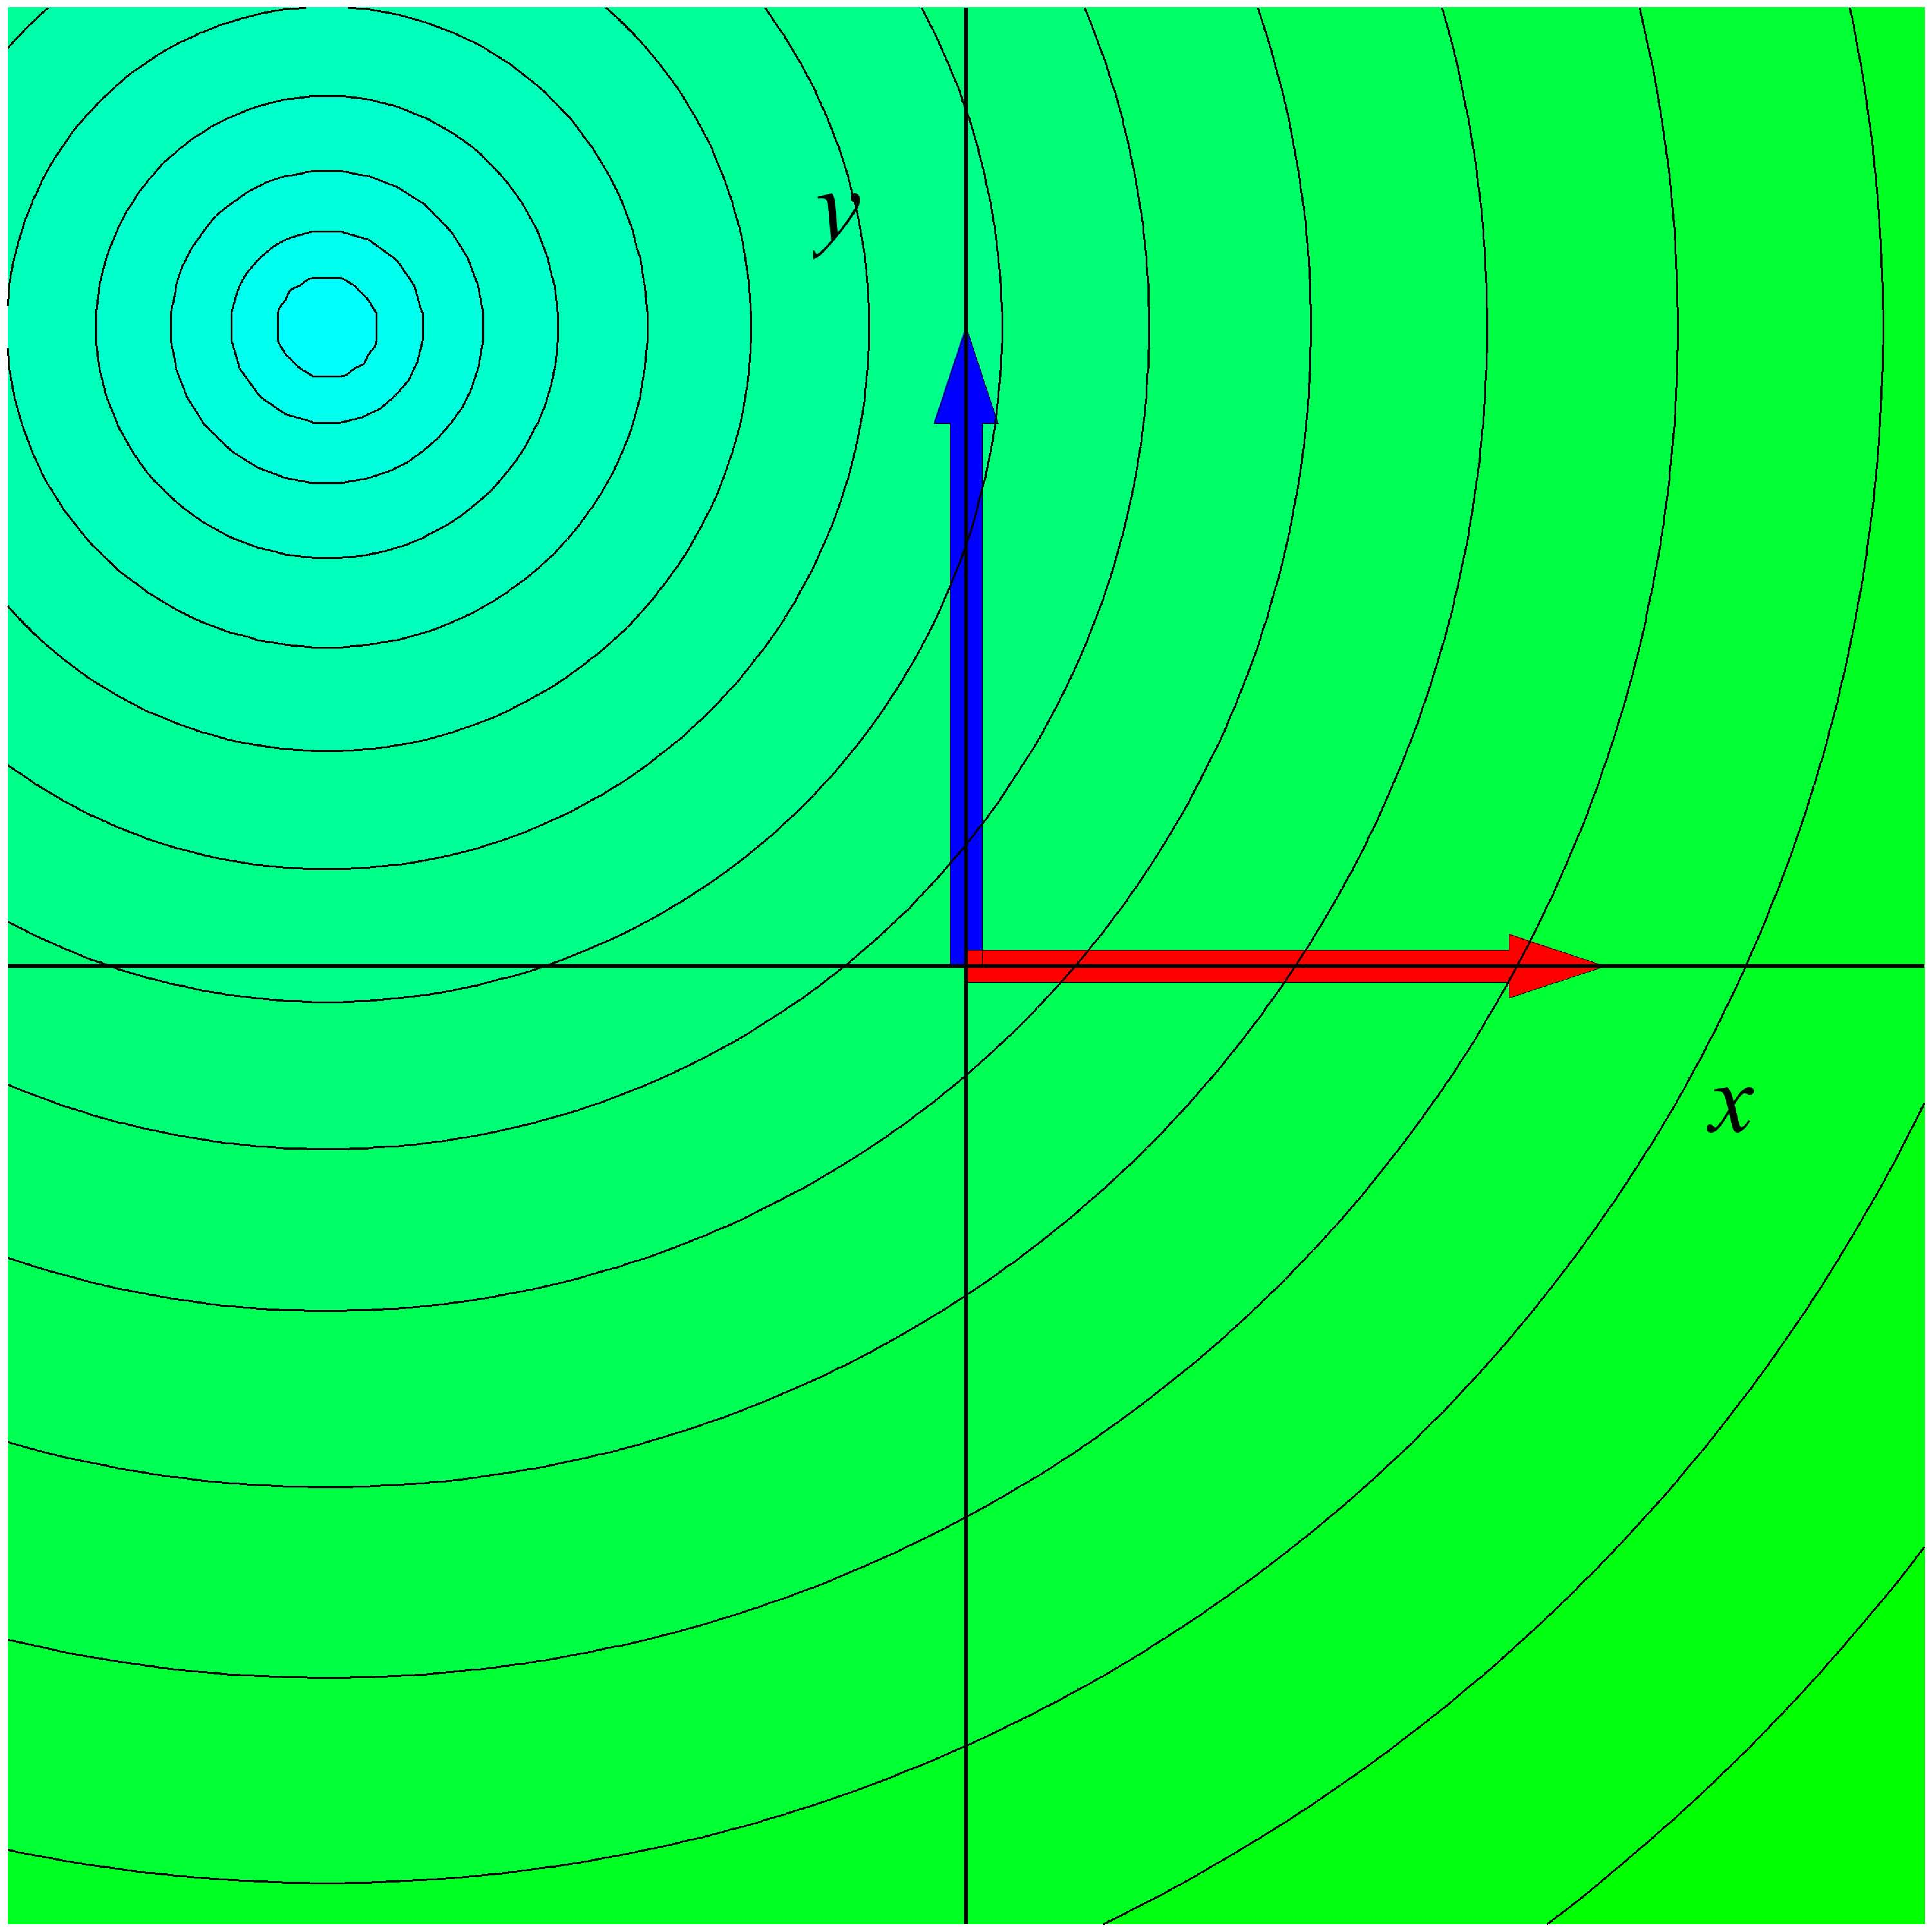
\includegraphics[height=25mm]{plotSqrtNiveau.pdf} \quad 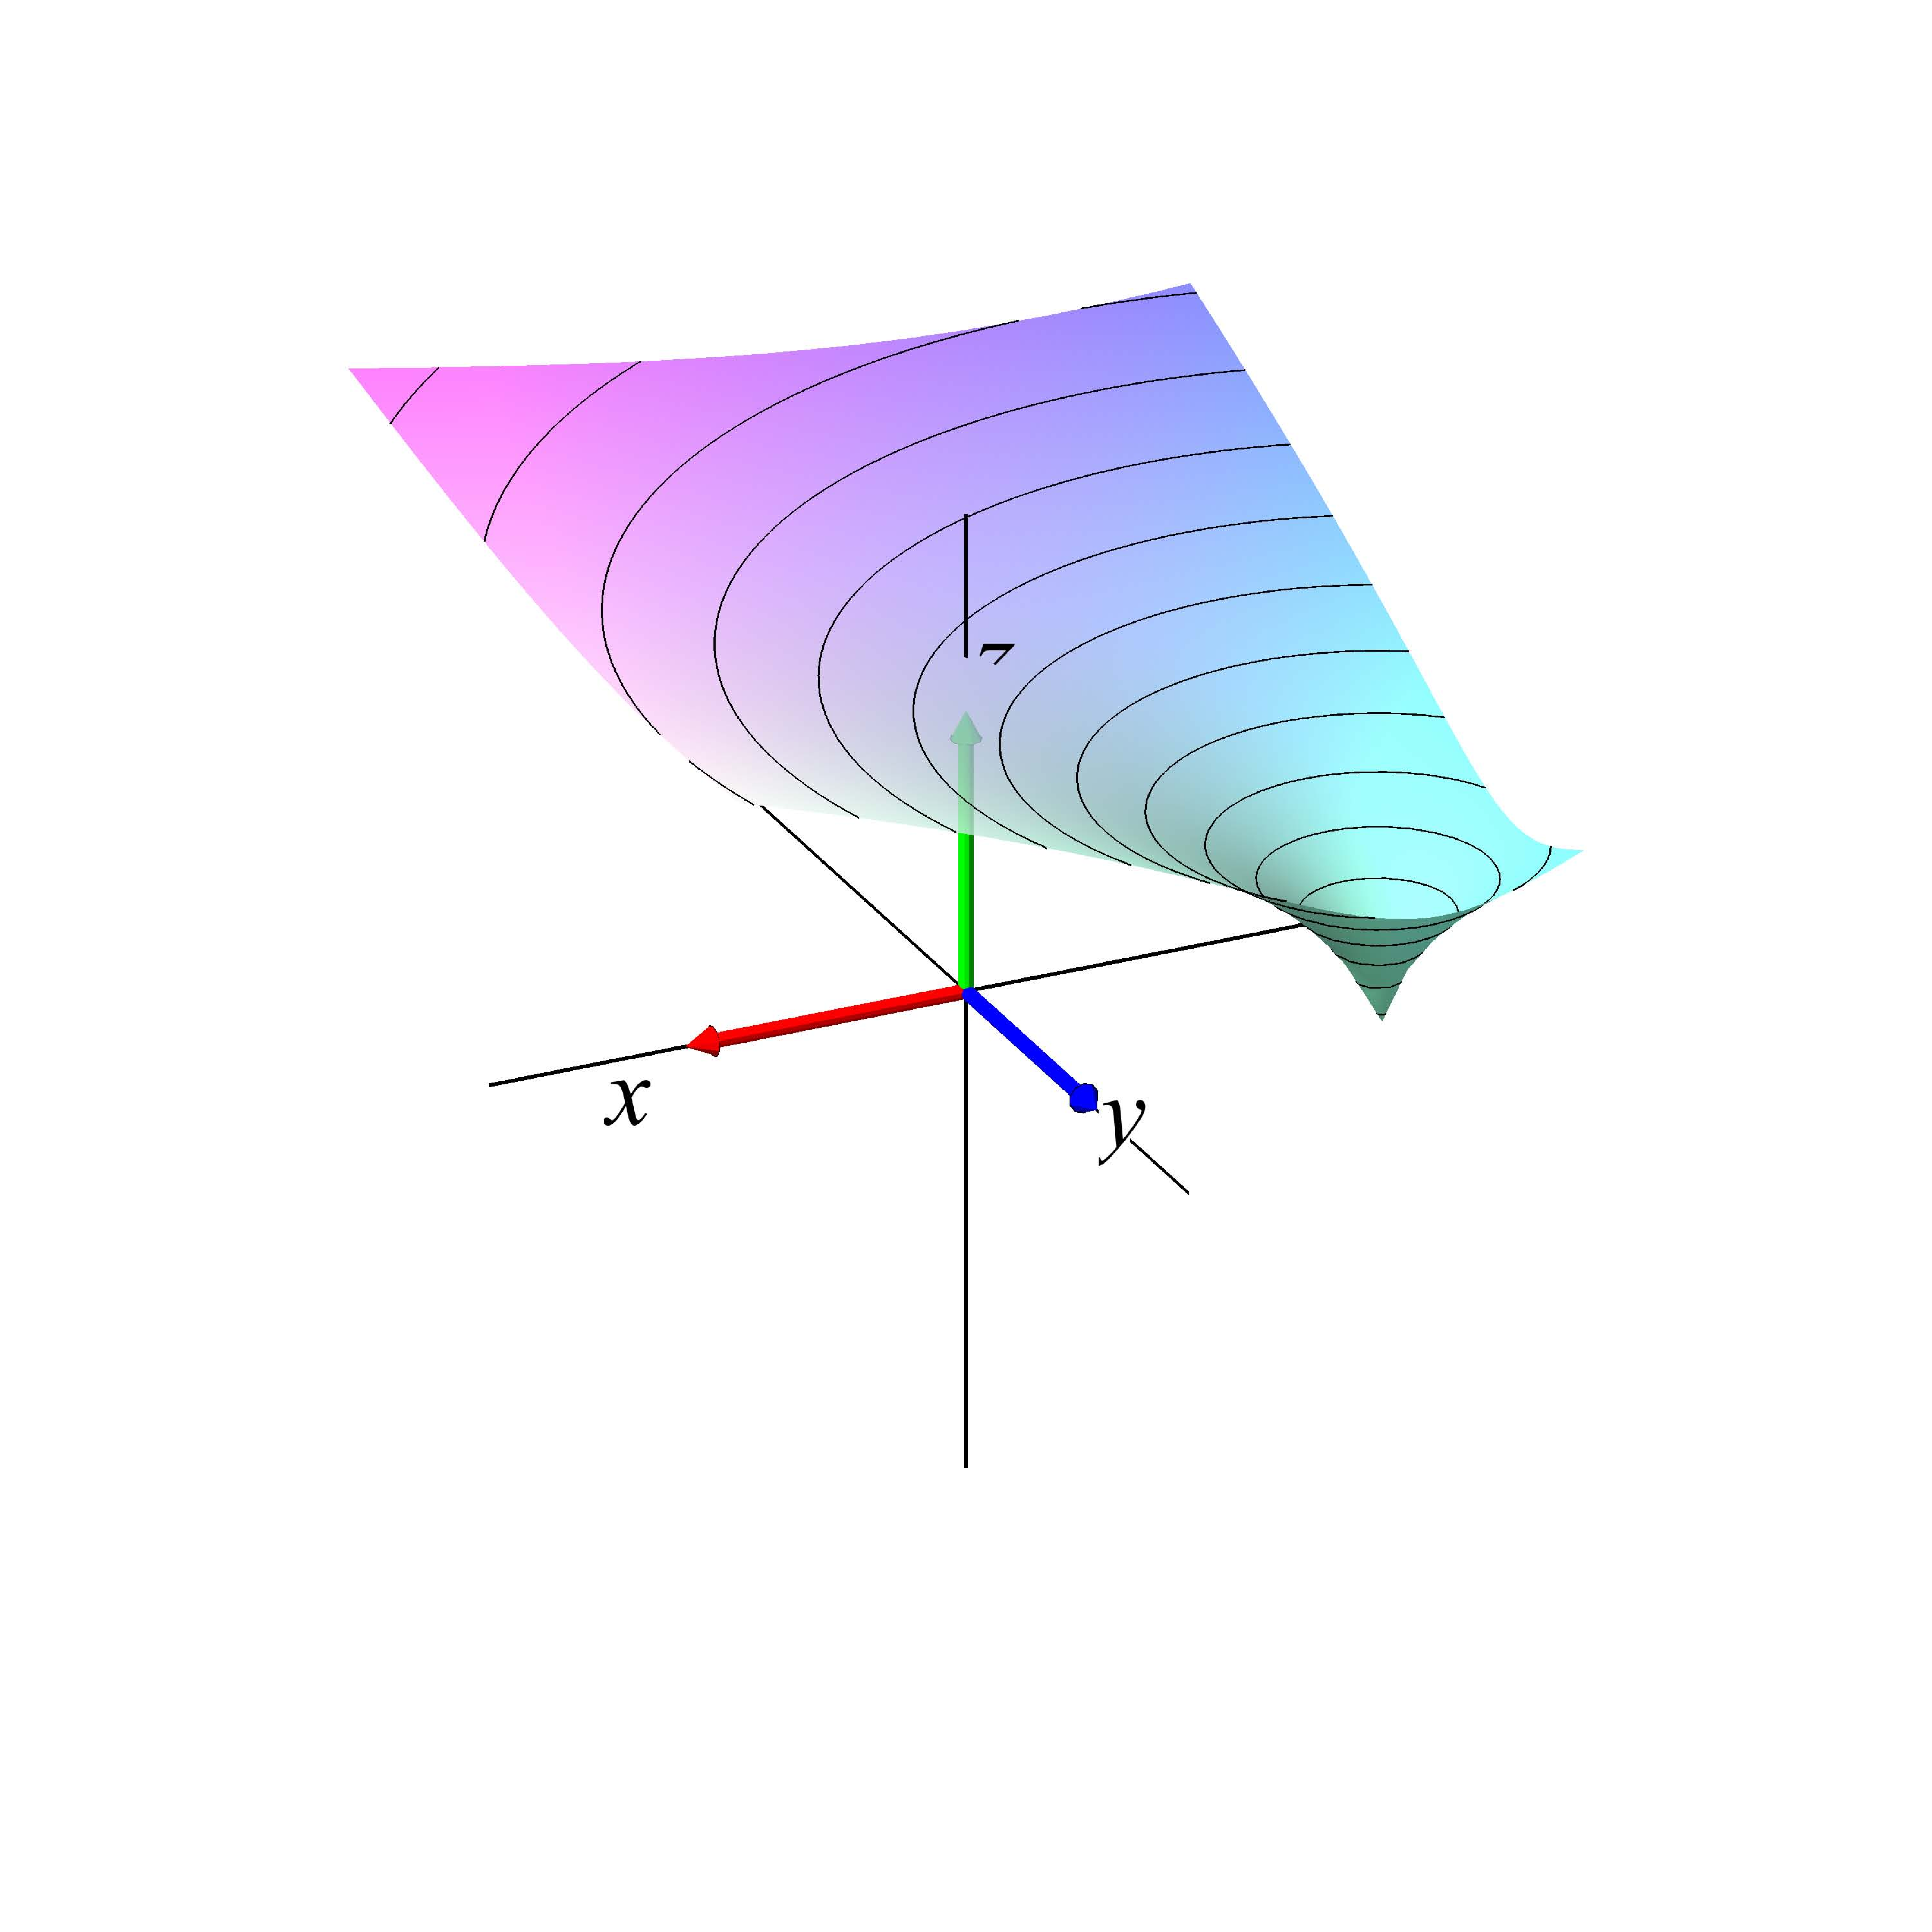
\includegraphics[height=80mm]{plotSqrtNiveauUP.pdf}}
\begin{center}
\caption{Grafen, niveau-kurverne, og højdesnitkurverne  for kvadratroden af afstandsfunktionen til punktet $(x_{0}, y_{0}) = (-1,1)$\, : \, $f(x, y) = \sqrt{\rho_{(x_{0}, y_{0})}(x,y)}\,$. } \label{figSqrt}
\end{center}
\end{figure}



%%%%%%%%%%%%%%%%%%%%%%%%%%%%%%%%%%%%%%%%%%%%%%%%%%%
%%%%%%%%%%%%%%%%%%%%%%%%%%%%%%%%%%%%%%%%%%%%%%%%%%%
%%%%%%%%%%%%%%%%%%%%%%%%%%%%%%%%%%%%%%%%%%%%%%%%%%%

\section{Differentiable funktioner af to variable} \label{Epsilon}
Langt de fleste af de funktioner vi betragter i Matematik 1 er differentiable i deres definitionsområder og af den grund også kontinuerte, som vi skal se nedenfor -- jævnfør tilsvarende for funktioner af \'{e}n variabel. \\

Differentiabilitet defineres som for funktioner af \'{e}n variabel, men her igen ved brug af de indførte epsilonfunktioner af to variable:

\begin{definition}[Differentiabilitet og partielle afledede]
En funktion $f(x,y)$ er differentiabel i $(x_{0}, y_{0}) \in \mathcal{D}m(f)$ hvis der findes \emph{to} konstanter $a$ og $b$ og en
epsilon-funktion $\varepsilon_{f}(x-x_{0},y-y_{0})$ sådan at
\begin{equation}
\begin{aligned}
f(x,y) = &f(x_{0}, y_{0}) + a\cdot (x-x_{0}) + b\cdot (y-y_{0}) \\
&\phantom{f(x,y) =}+ \rho_{(x_{0}, y_{0})}(x,y) \cdot \varepsilon_{f}(x-x_{0},y-y_{0}) \quad .
\end{aligned}
\end{equation}
Det er de to konstanter $a$ og $b$ vi herefter (når de findes, altså når $f(x,y)$ er differentiabel) kalder de \ind{partielle afledede}{partielle afledede} af $f$ i $(x_{0}, y_{0})$. De betegnes henholdsvis:
\begin{equation}
a = f'_{x}(x_{0}, y_{0}) \quad \textrm{og} \quad b = f'_{y}(x_{0}, y_{0})
\end{equation}
Med denne notation gælder altså -- når $f(x,y)$ er differentiabel i $(x_{0}, y_{0})$:
\begin{equation} \label{eqDifferentiabel}
\begin{aligned}
f(x,y) = &f(x_{0}, y_{0}) + f'_{x}(x_{0}, y_{0})\cdot (x-x_{0}) + f'_{y}(x_{0}, y_{0})\cdot (y-y_{0}) \\
&\phantom{f(x,y) =}+ \rho_{(x_{0}, y_{0})}(x,y) \cdot \varepsilon_{f}(x-x_{0},y-y_{0}) \quad .
\end{aligned}
\end{equation}
\end{definition}


\begin{definition}[Partielle afledede af partielle afledede] \label{defPartialPartial}
Hvis $f(x,y)$ er differentiabel i alle punkter $(x_{0}, y_{0})$ i et givet åbent område i $\mathcal{D}m(f) \subset \mathbb{R}^{2}$ siger vi, at $f(x,y)$ er differentiabel i hele området. Vi skriver så ofte de partielle afledede af $f(x,y)$ på følgende måde, idet de jo dermed selv er funktioner af de to \emph{variable} $(x_{0}, y_{0})$:
\begin{equation}
f'_{x}(x, y) = \frac{\partial}{\partial x}f(x,y) =  \frac{\partial f}{\partial x}(x,y)\quad \textrm{og} \quad  f'_{y}(x, y) = \frac{\partial}{\partial y}f(x,y) = \frac{\partial f}{\partial y}(x, y) \quad .
\end{equation}
Hvis disse partielle afledede af $f(x,y)$ selv er differentiable, kan vi fortsætte og finde de tilhørende \ind{partielle afledede af de partielle afledede}{partielle afledede af de partielle afledede}, etc. De benævnes på følgende måde:
\begin{equation}
\begin{aligned}
f''_{xx}(x, y) &= \frac{\partial}{\partial x}f'_{x}(x,y) =  \frac{\partial^{2} f}{\partial x \partial x}(x,y) \\
f''_{xy}(x, y) &= \frac{\partial}{\partial y}f'_{x}(x,y) =  \frac{\partial^{2} f}{\partial y \partial x}(x,y) \\
f''_{yx}(x, y) &= \frac{\partial}{\partial x}f'_{y}(x,y) =  \frac{\partial^{2} f}{\partial x \partial y}(x,y) \\
f''_{yy}(x, y) &= \frac{\partial}{\partial y}f'_{y}(x,y) =  \frac{\partial^{2} f}{\partial y \partial y}(x,y) \quad .
\end{aligned}
\end{equation}
\end{definition}




Hvordan finder vi så konkret de partielle afledede af en given funktion $f(x,y)$, f.eks. $f(x,y) = x\cdot \sin(y)$? Det er ikke svært:


\begin{theorem}[Hjælpefunktioner giver partielle afledede]
De partielle afledede af en funktion $f(x,y)$, der er differentiabel i $(x_{0}, y_{0})$ kan findes ved sædvanlig differentiation af to funktioner af \'{e}n variabel. Sæt
\begin{equation}
\begin{aligned}
f_{1}(x) &= f(x, y_{0}) \\
f_{2}(y) &= f(x_{0}, y) \quad.
\end{aligned}
\end{equation}
Så er funktionerne $f_{1}(x)$ og $f_{2}(y)$ to funktioner af hver \'{e}n variabel, henholdsvis $x$ og $y$, og de er begge differentiable i henholdsvis $x_{0}$ og $y_{0}$, og differentialkvotienterne er netop de partielle afledede:
\begin{equation}
f'_{x}(x_{0}, y_{0}) = f'_{1}(x_{0}) \quad \textrm{og} \quad f'_{y}(x_{0}, y_{0}) = f'_{2}(y_{0})
\end{equation}
Med andre ord: Ved at indføre de to hjælpefunktioner af \'{e}n variabel, $f_{1}(x)$ og $f_{2}(y)$, fås de partielle afledede af $f(x,y)$ ved at finde de sædvanlige differentialkvotienter af $f_{1}(x)$ og $f_{2}(y)$ i henholdsvis $x_{0}$ og $y_{0}$.
\end{theorem}
\begin{bevis}
Hvis vi sætter $y=y_{0}$ overalt i ligning (\ref{eqDifferentiabel}) får vi:
\begin{equation}
\begin{aligned}
f_{1}(x) = f(x,y_{0}) = &f_{1}(x_{0}) + f'_{x}(x_{0}, y_{0})\cdot (x-x_{0}) \\
&\phantom{f(x,y) =}+ \rho_{(x_{0}, y_{0})}(x,y_{0}) \cdot \varepsilon_{f}(x-x_{0},0) \quad ,
\end{aligned}
\end{equation}
sådan at koefficienten til faktoren $(x-x_{0})$ lige præcis er $f'_{x}(x_{0}, y_{0})$. Vi aflæser altså for det første, at $f_{1}(x)$ er differentiabel i $x_{0}$ og for det andet, at $ f'_{1}(x_{0}) = f'_{x}(x_{0}, y_{0})$. Og det var den ene halvdel af det vi skulle vise; den anden halvdel -- vedrørende $f'_{2}(y_{0}) = f'_{y}(x_{0}, y_{0})$ -- fås på helt tilsvarende måde.
\end{bevis}


\begin{example}[Bestemmelse af partielle afledede]
Vi vil bestemme de partielle afledede af funktionen $f(x,y) = 3\,x^{2} + 7\,y^{3} + 10\,x\,y^{7}$ i ethvert punkt $(x_{0}, y_{0})$ i $\mathbb{R}^{2}$. Vi opstiller først de to hjælpefunktioner $f_{1}(x) = f(x, y_{0})$ og $f_{2}(y) = f(x_{0}, y)$:
\begin{equation}
\begin{aligned}
f_{1}(x) &= 3\,x^{2} + 7\,y_{0}^{3} + 10\,x\,y_{0}^{7} \\
f_{2}(y) &= 3\,x_{0}^{2} + 7\,y^{3} + 10\,x_{0}\,y^{7} \quad.
\end{aligned}
\end{equation}
De to hjælpefunktioner har differentialkvotienterne henholdsvis:
\begin{equation}
\begin{aligned}
f_{1}'(x) &= 6\,x + 0 + 10\,y_{0}^{7} \quad \textrm{da $y_{0}$ jo er en konstant her,} \\
f_{2}'(y) &= 0 + 21\,y^{2} + 70\,x_{0}\,y^{6} \quad \textrm{da $x_{0}$ er en konstant} \quad.
\end{aligned}
\end{equation}
Heraf får vi dernæst hjælpefunktionernes differentialkvotienter i $x_{0}$ henholdsvis $y_{0}$:
\begin{equation}
\begin{aligned}
f_{1}'(x_{0}) &= 6\,x_{0} +  10\,y_{0}^{7}  = f'_{x}(x_{0}, y_{0})\\
f_{2}'(y_{0}) &= 21\,y_{0}^{2} + 70\,x_{0}\,y_{0}^{6} = f'_{y}(x_{0}, y_{0})  \quad.
\end{aligned}
\end{equation}
Heraf fås generelt, det vil sige for alle $(x,y)$ i $\mathbb{R}^{2}\,$:
\begin{equation}
\begin{aligned}
f'_{x}(x,y) &= 6\,x +  10\,y^{7}  \\
f'_{y}(x,y) &= 21\,y^{2} + 70\,x\,y^{6} \quad.
\end{aligned}
\end{equation}
\end{example}

\begin{exercise}
Vis (på samme måde som for differentiable funktioner af \'{e}n variabel), at hvis $f(x,y)$ er differentiabel i $(x_{0}, y_{0})$, så er de to konstanter $a$ og $b$, altså konstanterne $f'_{x}(x_{0}, y_{0})$ og $f'_{y}(x_{0}, y_{0})$, veldefinerede i følgende forstand: Der findes \emph{ikke} to forskellige par af
konstanter $a_{1}, b_{1}$ og $a_{2}, b_{2}$ og to epsilonfunktioner $\varepsilon_{1}$ og $\varepsilon_{2}$ sådan at der samtidig gælder:
\begin{equation}
\begin{aligned}
f(x,y) = &f(x_{0}, y_{0}) + a_{1}\cdot (x-x_{0}) + b_{1}\cdot (y-y_{0}) \\
&\phantom{f(x,y) =}+ \rho_{(x_{0}, y_{0})}(x,y) \cdot \varepsilon_{1}(x-x_{0},y-y_{0}) \\ \\
f(x,y) = &f(x_{0}, y_{0}) + a_{2}\cdot (x-x_{0}) + b_{2}\cdot (y-y_{0}) \\
&\phantom{f(x,y) =}+ \rho_{(x_{0}, y_{0})}(x,y) \cdot \varepsilon_{2}(x-x_{0},y-y_{0}) \quad .
\end{aligned}
\end{equation}
\end{exercise}



\begin{exercise}
Bestem samtlige partielle afledede af de partielle afledede i ethvert punkt $(x,y)$ for funktionen $f(x,y) = 3\,x^{2} + 7\,y^{3} + 10\,x\,y^{7}$.
\end{exercise}

\begin{exercise}
Bestem samtlige partielle afledede af de partielle afledede i ethvert punkt $(x,y)$ for funktionen $f(x,y) = \cos(3x)\cdot\sin(3y)$.
\end{exercise}


Den opmærksomme opgaveløser vil have observeret (f.eks. i opgaverne ovenfor) at $f''_{xy}(x, y)$ og $f''_{yx}(x, y)$ typisk er ens!
Det er ikke nogen tilfældighed, det gælder sædvanligvis at man kan nøjes med at beregne den ene af de to dobbeltafledede:

\begin{theorem}[De blandede dobbeltafledede er ens] \label{thmBlandDobbelt}
Hvis alle de $4$ dobbelt afledede af en given funktion $f(x,y)$ er kontinuerte i et åbent område, så gælder i hele området:
\begin{equation}
f''_{xy}(x,y) = f''_{yx}(x,y) \quad .
\end{equation}
\end{theorem}

\begin{exercise}
Vis (på samme måde som for funktioner af \'{e}n variabel) at: Hvis en funktion $f(x, y)$ af to variable er differentiabel i et punkt $(x_{0}, y_{0})$, så er funktionen også kontinuert i dette punkt. Vis også med et eksempel, at hvis en funktion er kontinuert i $(x_{0}, y_{0})$, så behøver den ikke at være differentiabel i $(x_{0}, y_{0})$. Se f.eks. på $\rho_{(x_{0}, y_{0})}(x,y)$.
\end{exercise}

Den opmærksomme vil også have noteret, at vi mangler en overvejelse: Hvis $f(x,y)$ er differentiabel i et punkt $(x_{0}, y_{0})$, så findes de partielle afledede
i konsekvens af differentiabiliteten og de kan bestemmes ved hjælp af de differentiable hjælpefunktioner $f_{1}(x)$ og $f_{2}(y)$. Man kan nu med god grund  spørge: Hvis de to hjælpefunktioner findes  for en given funktion $f(x,y)$,  og det viser sig, at de er differentiable i henholdsvis $x_{0}$ og $y_{0}$, betyder det så, at $f(x,y)$ er differentiabel i $(x_{0}, y_{0})$? \\

Følgende sætning kaster lys over dette spørgsmål:

\begin{theorem}[Fra partielle afledede til differentiabilitet] \label{thmPartiel2Dif}
Hvis $f(x,y)$ har partielle afledede (fundet via hjælpefunktionerne $f_{1}(x)$ og $f_{2}(y)$)  i et åbent område $A$ indeholdende $(x_{0}, y_{0})$, og hvis de partielle afledede af $f(x,y)$ begge er kontinuerte i $A$, så er $f(x,y)$ differerentiabel.
\end{theorem}

At der nødvendigvis må være en ekstra betingelse i sætning \ref{thmPartiel2Dif} følger af eksemplet her:

\begin{example}[Differentiable hjælpefunktioner er ikke nok]
Vi ser på $0$-udvidelsen af følgende funktion:
\begin{equation}
f(x,y) = \frac{x\,y^{2}}{x^{2} + y^{4}} \quad .
\end{equation}
Den funktion er ikke differentiabel i $(0,0)$ -- den er nemlig ikke engang kontinuert i $(0,0)$ (!) (Hvorfor ikke?) Ikke desto mindre findes de to hjælpefunktioner
\begin{equation}
\begin{aligned}
f_{1}(x) &= f(x, 0) = 0 \\
f_{2}(y) &= f(0, y) = 0 \quad,
\end{aligned}
\end{equation}
og som det ses, er de begge to særdeles differentiable i $(0,0)$. Selv om hjælpefunktionerne er differentiable behøver den aktuelle
funktion selv ikke at være differentiabel.
\end{example}




%%%%%%%%%%%%%%%%%%%%%%%%%%%%%%%%%%%%%%%%%%%%%%%%%%%
%%%%%%%%%%%%%%%%%%%%%%%%%%%%%%%%%%%%%%%%%%%%%%%%%%%
%%%%%%%%%%%%%%%%%%%%%%%%%%%%%%%%%%%%%%%%%%%%%%%%%%%



\section{Det approksimerende første-grads-polynomium}

Som for funktioner af \'{e}n variabel kan vi trunkere udtrykket i ligning (\ref{eqDifferentiabel}) ved simpelthen at fjerne 'epsilon-funktions-delen' hvorved vi står tilbage med et førstegrads-polynomium i de to variable $x$ og $y$:
\begin{equation}
P_{1, (x_{0}, y_{0})}(x,y) = f(x_{0}, y_{0}) + f'_{x}(x_{0}, y_{0})\cdot (x-x_{0}) + f'_{y}(x_{0}, y_{0})\cdot (y-y_{0}) \quad .
\end{equation}
Funktionen $P_{1, (x_{0}, y_{0})}(x,y)$ kaldes det approksimerende første-gradspolynomium for $f(x,y)$ med udviklingspunkt $(x_{0}, y_{0})$.\\

Læg mærke til, at $P_{1, (x_{0}, y_{0})}(x,y)$ virkelig \emph{er} et første-grads-polynomium i de to variable $x$ og $y$ fordi de højst optræder med potensen $1$ og alle andre faktorer og addender er konstanter.

\begin{example}[Paraboloide med tangentplan]
Vi ser på funktionen
\begin{equation}
f(x,y) = 1 - \frac{1}{2}x^{2} - \frac{1}{2}y^{2} \quad.
\end{equation}
Så er
\begin{equation}
\begin{aligned}
f'_{x}(x_{0}, y_{0}) &= -x_{0}\\
f'_{y}(x_{0}, y_{0}) &= - y_{0} \quad,
\end{aligned}
\end{equation}
sådan at
\begin{equation}
\begin{aligned}
P_{1, (x_{0}, y_{0})}(x,y) &=  f(x_{0}, y_{0}) - x_{0}\cdot(x-x_{0}) - y_{0}\cdot (y-y_{0}) \\
&= 1 - \frac{1}{2}x_{0}^{2} - \frac{1}{2}y_{0}^{2} - x\cdot x_{0} + x_{0}^{2} - y\cdot y_{0} + y_{0}^{2} \\
&= 1 + \frac{1}{2}x_{0}^{2} + \frac{1}{2}y_{0}^{2} - x\cdot x_{0} - y\cdot y_{0} \quad .
\quad.
\end{aligned}
\end{equation}
Specielt får vi med udviklingspunktet $(x_{0}, y_{0}) = (1, -1)$:
\begin{equation}
P_{1, (1, -1)}(x,y) = y - x + 2 \quad .
\end{equation}
Se figur \ref{figParabPlan}, hvor grafen for dette approksimerende første-gradspolynomium for $f(x,y)$ er plottet sammen med grafen for
funktionen selv. Højde-snit-kurverne og niveau-kurverne er ligeledes gengivet for begge funktionerne. I og omkring det markerede udviklingspunkt er funktionerne
meget ens - grafen for det approksimerende førstegrads-polynomium med udviklingspunkt $(x_{0}, y_{0})$ fortjener helt klart at blive kaldt \ind{tangentplan}{tangentplanen} til grafen for $f(x,y)$ i punktet $(x_{0}, y_{0}, f(x_{0}, y_{0})$.
\end{example}

\begin{definition}[Tangentplan til grafen for en funktion af to variable]
Givet en differentiabel funktion $f(x,y)$. Tangentplanen til grafen for $f(x,y)$ i punktet $(x_{0}, y_{0}, f(x_{0}, y_{0}))$ er givet ved ligningen:
\begin{equation}
z = P_{1, (x_{0}, y_{0})}(x,y) \quad,
\end{equation}
hvor højresiden er det approksimerende polynomium af første grad for $f(x,y)$ med udviklingspunkt $(x_{0}, y_{0})$.
\end{definition}



\begin{figure}[h]
\centerline{
\includegraphics[height=90mm]{plotParabPlanUP.pdf} \quad 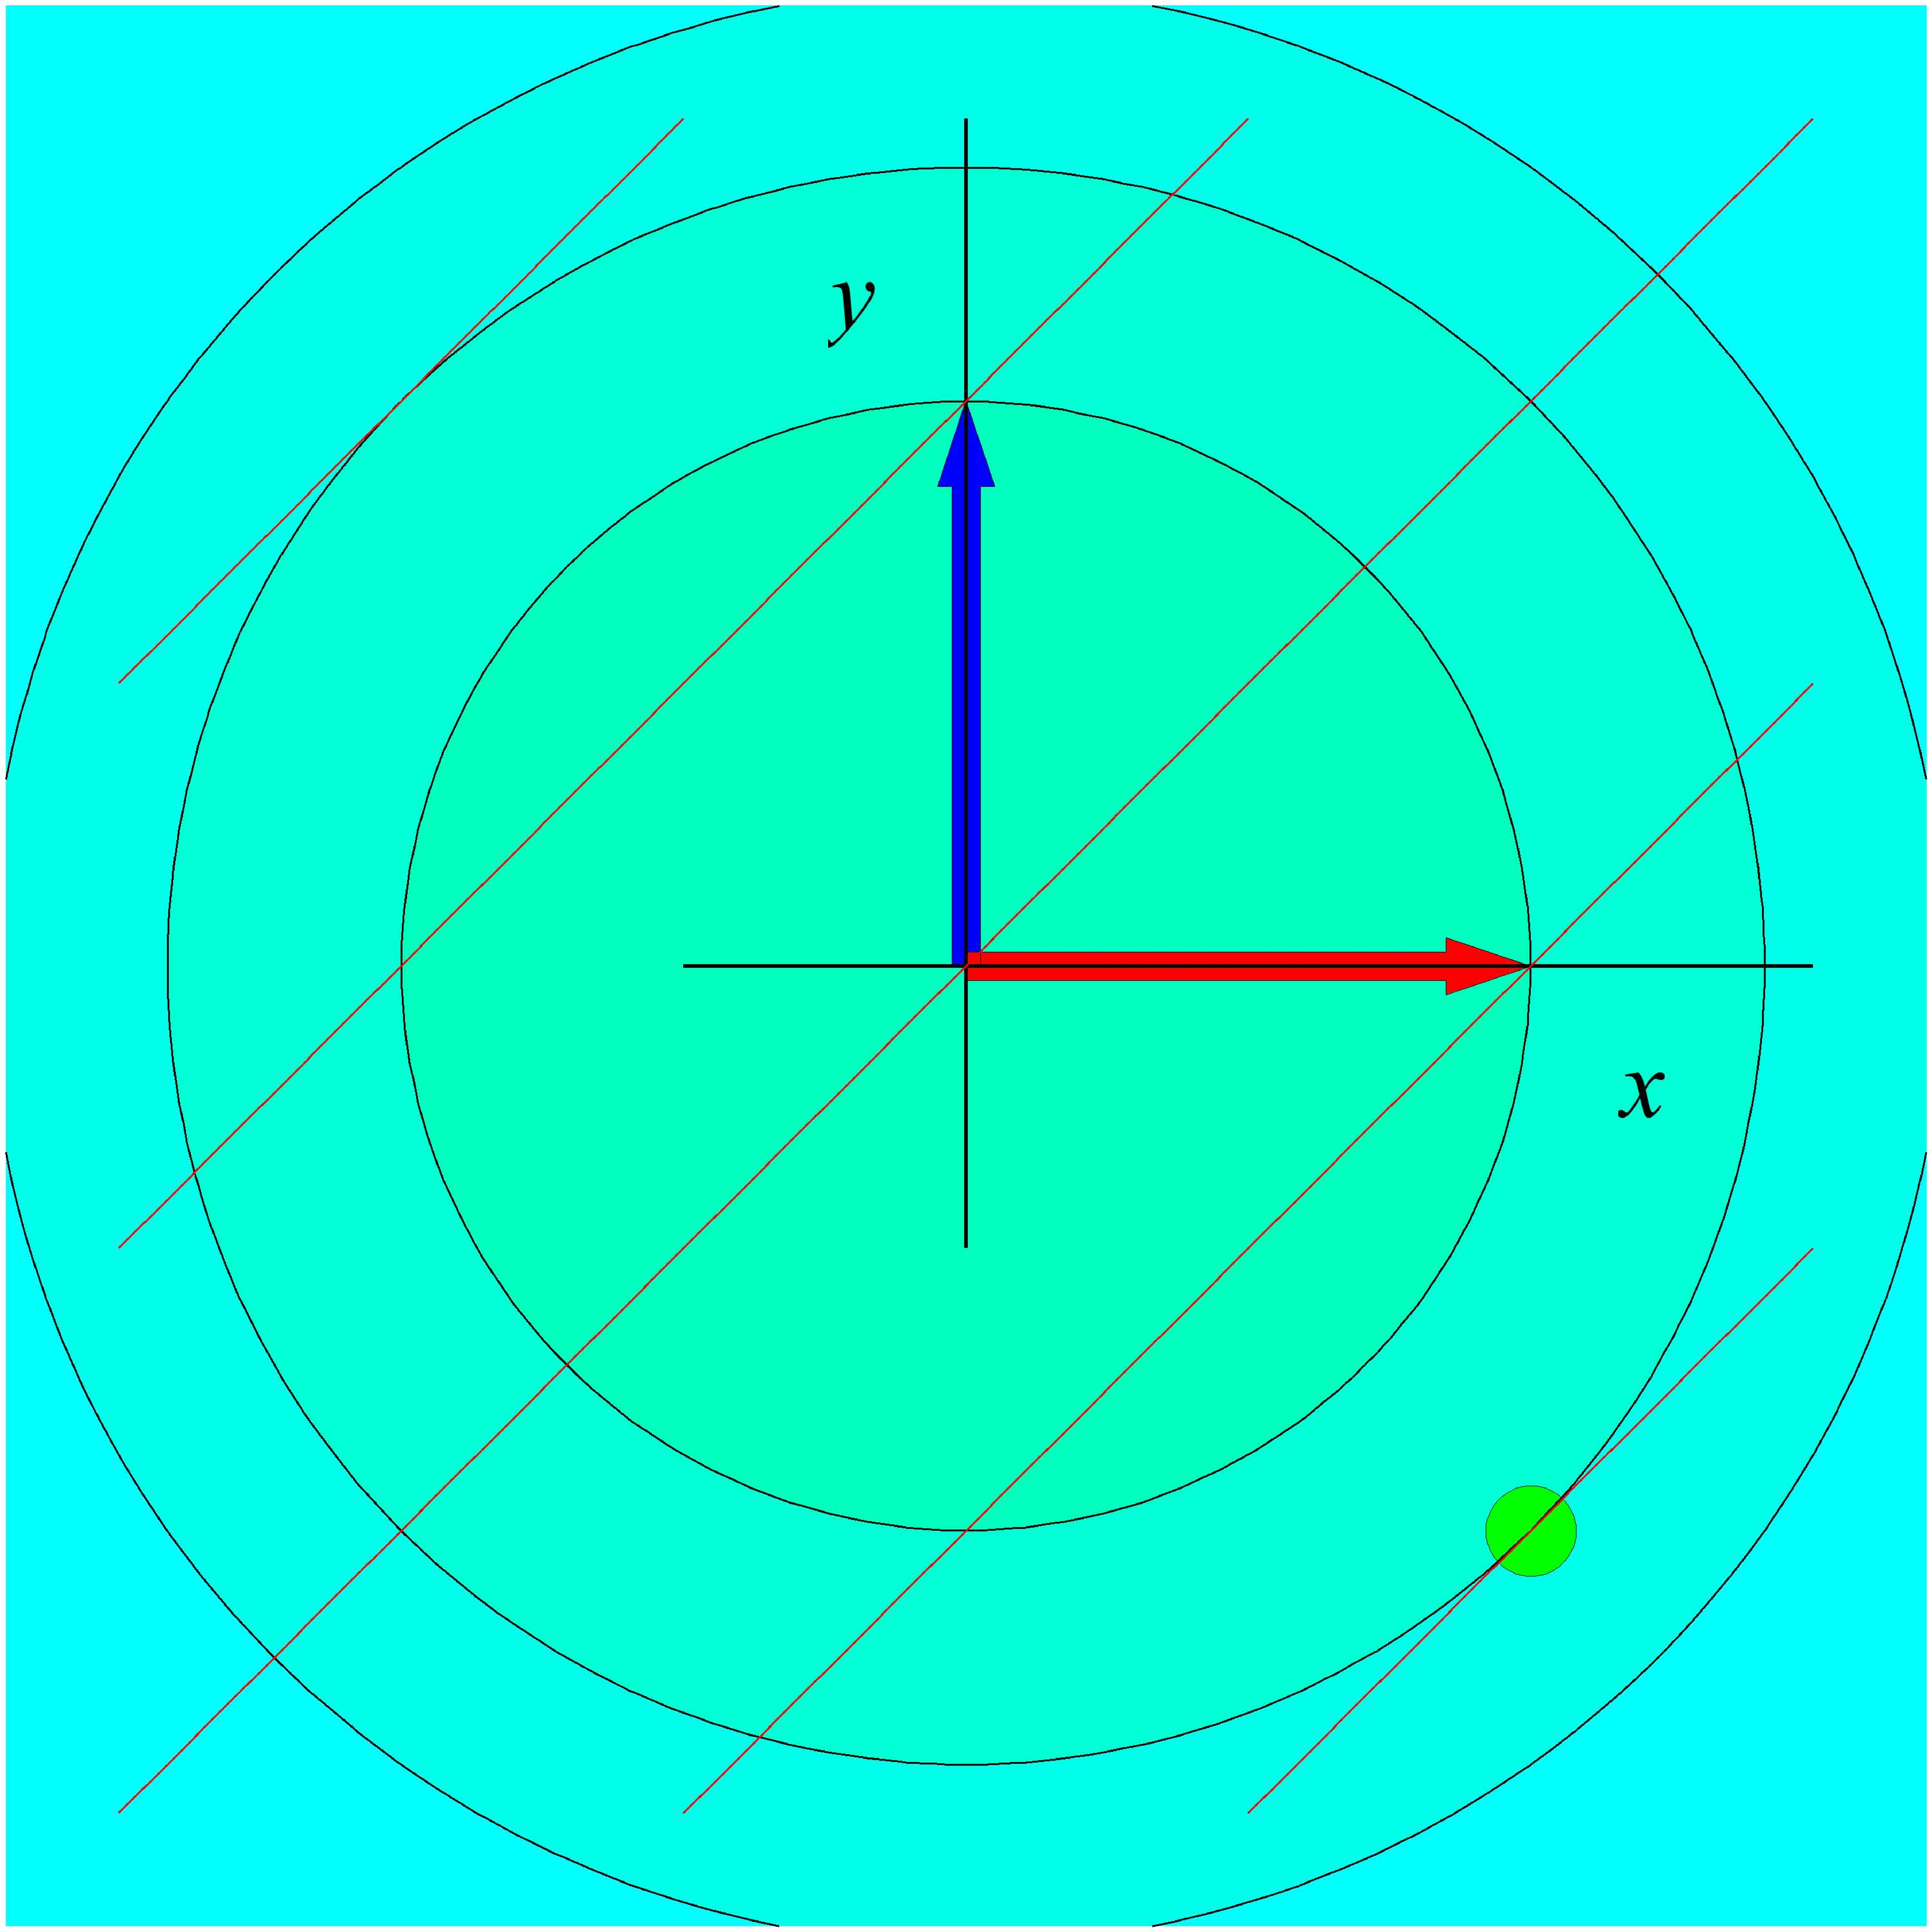
\includegraphics[height=35mm]{plotParabPlanNiveau.pdf}}
\begin{center}
\caption{Tangentplanen approksimerer grafen over udviklingspunktet og niveaulinjerne for det approksimerende førstegradspolynomium approksimerer niveaulinjerne for funktionen omkring udviklingspunktet i $(x, y)$-planen} \label{figParabPlan}
\end{center}
\end{figure}


\begin{exercise}
Bestem det approksimerende første-grads-polynomium for følgende funktion i ethvert punkt $(x_{0}, y_{0})$:
\begin{equation}
f(x,y) = \cos(3x)\cdot \sin(3y) \quad .
\end{equation}
\end{exercise}



%%%%%%%%%%%%%%%%%%%%%%%%%%%%%%%%%%%%%%%%%%%%%%%%%%%
%%%%%%%%%%%%%%%%%%%%%%%%%%%%%%%%%%%%%%%%%%%%%%%%%%%
%%%%%%%%%%%%%%%%%%%%%%%%%%%%%%%%%%%%%%%%%%%%%%%%%%%



\section{Partielle afledede af sammensatte funktioner}

Sammensatte funktioner af to variable optræder i rigtig mange anvendelser,
lige fra GPS teknologi til geologi og termodynamik. \\

En sammensat funktion af to variable
fås typisk således: Lad $f(x,y)$ være en funktion af to variable, hvor $(x,y) \in \mathcal{D}m(f) \subset \mathbb{R}^{2}$ og lad $p(u,v)$
og $q(u,v)$ være \emph{to} andre funktioner af to variable, hvor vi så antager, at $(u,v) \in \mathcal{D}m(p) \cap \mathcal{D}m(q) \subset \mathbb{R}^{2}$. Antager vi nu yderligere, at $(u,v)$ tilhører et område $A$ i $\mathbb{R}^{2}$ sådan at der gælder, at \emph{værdierne} af $p(u,v)$ og $q(u,v)$ ligger i definitionsmængden for $f(x,y)$ i den forstand, at $(p(u,v), q(u,v)) \in \mathcal{D}m(f)$ for $(u,v) \in A$,
så er den sammensatte funktion
\begin{equation}
h(u,v) = f(p(u,v), q(u,v)) \quad \textrm{veldefineret for alle} \quad (x,y) \in A \quad.
\end{equation}

Vi vil sædvanligvis kun se på sammensatte funktioner som er definerede i hele planen, sådan at  $A = \mathbb{R}^{2}$.

\begin{example}[Sammensatte funktioner af to variable]
Lad $f(x,y)$, $p(u,v)$, og $q(u,v)$ være bestemt ved de angivne funktioner nedenfor.  Så fås de tilsvarende sammensatte funktioner $h(u,v)$ ved at sætte $x= p(u,v)$, $y=q(u,v)$, og $h(u,v) = f(x,y) = f(p(u,v), q(u,v))$ i de respektive definitions-områder (de anføres ikke her):
\begin{equation}
\begin{array}{lllllll}
  f(x,y) = x+y & , & p(u,v) = 2u \cdot v  & , & q(u,v)= u^{2} + v^{2}& , & h(u,v) = (u + v)^{2}\\
  f(x,y) = y\cdot\e^{x} & , & p(u,v) = \ln(uv) & , & q(u,v)= 1/uv & , & h(u,v) = 1 \\
  f(x,y) = \sqrt{x + y} & , & p(u,v) = u^{4} & , & q(u,v)= 8\,u^{4}& , & h(u,v) = 3\cdot u^{2}\\
\end{array}
\end{equation}
\end{example}

\begin{theorem}[Kædereglen i planen] \label{thmChain2VarA}
Lad $f(x,y)$, $p(u,v)$, og $q(u,v)$ være tre differentiable funktioner - hver af to variable.
Lad $h(u,v)$ betegne den sammensatte funktion
\begin{equation}
h(u,v) = f(p(u,v), q(u,v)) \quad .
 \end{equation}
Så kan de partielle afledede af $h(u,v)$ udtrykkes ved hjælp af dels de partielle afledede af $f(x,y)$, dels de partielle afledede af $p(u,v)$, og dels de partielle afledede af $q(u,v)$. Vi vil udtrykke de partielle afledede af $h(u,v)$ i $(u_{0}, v_{0})$ så vi sætter $x_{0}= p(u_{0},v_{0})$ og $y_{0}= q(u_{0},v_{0})$.

 Så har vi:
\begin{equation}
\begin{aligned}
h'_{u}(u_{0},v_{0}) &=  f'_{x}(x_{0}, y_{0})\cdot p'_{u}(u_{0}, v_{0}) + f'_{y}(x_{0}, y_{0})\cdot q'_{u}(u_{0}, v_{0})\\
h'_{v}(u_{0},v_{0}) &=  f'_{x}(x_{0}, y_{0})\cdot p'_{v}(u_{0}, v_{0}) + f'_{y}(x_{0}, y_{0})\cdot q'_{v}(u_{0}, v_{0}) \quad .
\end{aligned}
\end{equation}
\end{theorem}
\begin{bevis}
Resultatet følger efter præcis samme opskrift som beviset for differentiation af den sammensatte funktion $f(g(x))$ af \'{e}n variabel -- der er bare lidt flere konstanter og funktioner at holde styr på.
\end{bevis}



\begin{exercise}
Bestem de partielle afledede i ethvert punkt $(u,v)$ for hver af de sammensatte funktioner nedenfor -- dels ved at beregne dem direkte ud fra det givne eksplicitte udtryk for $h(u,v)$ og dels ved at benytte kædereglen og de parteille afledede af ingredienserne i $h(u,v)$, altså de partielle afledede af $f(x,y)$, $p(u,v)$ og $q(u,v)$.
\begin{equation}
\begin{array}{lllllll}
  f(x,y) = x+y & , & p(u,v) = 2u \cdot v  & , & q(u,v)= u^{2} + v^{2}& , & h(u,v) = (u + v)^{2}\\
  f(x,y) = y\cdot\e^{x} & , & p(u,v) = \ln(uv) & , & q(u,v)= 1/uv & , & h(u,v) = 1 \\
  f(x,y) = \sqrt{x + y} & , & p(u,v) = u^{4} & , & q(u,v)= 8\,u^{4}& , & h(u,v) = 3\cdot u^2\\
\end{array}
\end{equation}
\end{exercise}



\begin{aha}
Læg mærke til, at hver af de partielle afledede af den sammensatte funktion $h(u,v) = f(p(u,v), q(u,v))$ i et punkt $(u_{0}, v_{0})$ effektivt kan udtrykkes ved prikprodukter hvori indgår en fælles faktor, nemlig vektoren $\left(f'_{x}(x_{0}, y_{0})\, , \,\,f'_{y}(x_{0}, y_{0})\right)$ hvor $x_{0}= p(u_{0}, v_{0})$ og $y_{0}= q(u_{0}, v_{0})$:
\begin{equation*}
\begin{aligned}
h'_{u}(u_{0},v_{0}) &=  \left(f'_{x}(x_{0}, y_{0})\, , \,\, f'_{y}(x_{0}, y_{0})\right) \bm{\cdot} \left(p'_{u}(u_{0}, v_{0})\, , \,\,q'_{u}(u_{0}, v_{0})\right)\\
h'_{v}(u_{0},v_{0}) &=  \left(f'_{x}(x_{0}, y_{0})\, , \,\, f'_{y}(x_{0}, y_{0})\right) \bm{\cdot} \left(p'_{v}(u_{0}, v_{0})\, , \,\, q'_{v}(u_{0}, v_{0}) \right)\quad .
\end{aligned}
\end{equation*}
\end{aha}


\subsection{Gradientvektorer} \label{subsecGradientVec}

\begin{definition}[Gradientvektor]
Lad $f(x,y)$ betegne en differentiabel funktion af to variable. De partielle afledede af $f(x,y)$ i et punkt $(x_{0}, y_{0})$ definerer
\ind{gradientvektoren for $f(x,y)$}{gradientvektoren for $f(x,y)$} i $(x_{0}, y_{0})$ på følgende måde:
\begin{equation}
{\bm{\nabla}}f(x_{0}, y_{0}) = \left(f'_{x}(x_{0}, y_{0})\, , \, \, f'_{y}(x_{0}, y_{0}) \right) \quad .
\end{equation}
På denne måde får vi altså defineret en ganske bestemt vektor i ethvert punkt, hvor $f(x,y)$ er differentiabel:
\begin{equation}
{\bm{\nabla}}f(x,y) = \left(f'_{x}(x,y)\, , \, \, f'_{y}(x,y) \right) \quad .
\end{equation}
\end{definition}

Hvis vi for ethvert fodpunkt $(x_{0}, y_{0})$ afsætter gradientvektoren ${\bm{\nabla}}f(x_{0},y_{0})$ for $f(x,y)$ ud fra det fodpunkt i planen $\mathbb{R}^{2}$ får vi konstrueret \ind{gradientvektorfelt}{gradientvektorfeltet} for $f(x,y)$.

\begin{exercise}
Bestem gradientvektorfeltet  i ethvert punkt $(x,y)$ for hver af følgende funktioner i deres respektive definitionsmængder:
$f(x,y) = x+y$, $f(x,y) = y\cdot\e^{x}$,  og $f(x,y) = \rho_{x_{0}, y_{0}}^{2}(x,y)$.
\end{exercise}

Ved hjælp af gradientvektorfeltet ${\bm{\nabla}}f(x,y)$ for $f(x,y)$ kan vi nu formulere de partielle afledede af den sammensatte funktion
$h(u,v) = f(p(u,v), q(u,v))$ lidt smartere:

\begin{theorem}[Kædereglen udtrykt med gradienten af $f(x,y)$] \label{thmChain2VarB}
Lad $f(x,y)$, $p(u,v)$, og $q(u,v)$ være tre differentiable funktioner - hver af to variable.
Lad $h(u,v)$ betegne den sammensatte funktion
\begin{equation}
h(u,v) = f(p(u,v), q(u,v)) \quad .
 \end{equation}
Så kan de partielle afledede af $h(u_{0},v_{0})$ med hensyn til henholdsvis $u$ og $v$ i $(u_{0},v_{0})$ udtrykkes ved gradienten af $f(x,y)$ i $(x_{0}, y_{0}) = (\,p(u_{0},v_{0}), q(u_{0},v_{0})\,)\,$:
\begin{equation} \label{eqGeneralChain}
\begin{aligned}
h'_{u}(u_{0},v_{0}) &= {\bm{\nabla}}f(x_{0}, y_{0}) \bm{\cdot} \left(p'_{u}(u_{0},v_{0}), q'_{u}(u_{0},v_{0}) \right) \\
h'_{v}(u_{0},v_{0}) &= {\bm{\nabla}}f(x_{0}, y_{0}) \bm{\cdot} \left(p'_{v}(u_{0},v_{0}), q'_{v}(u_{0},v_{0}) \right) \quad .
\end{aligned}
\end{equation}
\end{theorem}


%%%%%%%%%%%%%%%%%%%%%%%%%%%%%%%%%%%%%%%%%%%%%%%%%%%
%%%%%%%%%%%%%%%%%%%%%%%%%%%%%%%%%%%%%%%%%%%%%%%%%%%
\subsection{Kædereglen 'langs' kurver i planen}
Hvis funktionerne $p(u,v)$ og $q(u,v)$ kun afhænger af den ene variable $u$ kan vi selvfølgelig betegne funktionerne med henholdsvis  $p(u)$ og $q(u)$.
Den sammensattte funktion $h(u) = f(p(u), q(u))$ -- hvor $f(x,y)$ er en givet differerentiabel funktion i planen -- angiver så de funktionsværdier, som $f(x,y)$ antager \emph{langs den kurve} i planen, som er givet ved de to funktioner $p(u)$ og $q(u)$:

\begin{definition}[Parametriserede kurver i planen]
En \ind{kurve i planen}{kurve i planen} består af en punktmængde $\mathcal{C}$ i planen, som vi vil antage er givet ved to funktioner $p(u)$ og $q(u)$ på følgende måde:
\begin{equation}
\mathcal{C}_{\mathbf{r}}\quad : \quad \mathbf{r}(u) = (p(u), q(u)) \quad \textrm{hvor} \quad u \in \, ]\alpha, \beta[ \, \subset \mathbb{R} \quad .
\end{equation}
Det vil sige, at kurven er en parametriseret punktmængde med stedvektorerne $\mathbf{r}(u)$ og parameteren $u$ i et givet interval.
Kurven er \ind{differentiabel kurve}{differentiabel} hvis de to funktioner $p(u)$ og $q(u)$ begge er differentiable i hele intervallet $\,]\alpha, \beta[ \,$.\\

Den parametriserede kurve siges at være \ind{regulær kurve}{regulær}, hvis $\mathbf{r}'(u) \neq \mathbf{0}$ for alle $u \in \, ]\alpha, \beta[\,$.
\end{definition}


\begin{theorem}[Tangent til kurve]
Lad $\mathcal{C}_{\mathbf{r}}$ betegne en differentiabel kurve med parameterfremstillingen $\mathbf{r}(u)$ og antag at $\mathbf{r}'(u_{0}) \neq (0, 0)$.
Tangenten $L_{u_{0}}$ (igennem punktet $\mathbf{r}(u_{0})$) til  $\mathcal{C}_{\mathbf{r}}$ er så givet ved følgende parameterfremstilling:
\begin{equation}
L_{u_{0}}\quad : \quad \mathbf{T}(t) =  \mathbf{r}(u_{0}) + t \cdot \mathbf{r}'(u_{0}) \quad \textrm{hvor} \quad t \in \mathbb{R} \quad.
\end{equation}
\end{theorem}
\begin{bevis}
Vi nøjes med at se på det tilfælde hvor $p(u)$ er meget elementær: $p(u) = u$. Så er $\mathcal{C}_{\mathbf{r}}$ simpelthen grafen for funktionen $q(x)$ i $(x,y)$-planen. Grafen for den funktion har en tangent i punktet $(x_{0}, q(x_{0})$, som er givet ved ved det velkendte udtryk: $y = q(x_{0}) + q'(x_{0})(x-x_{0})$. En parameterfremstilling for den tangent er derfor:
\begin{equation}
\begin{aligned}
\mathbf{T}(t) &= (x_{0}, q(x_{0})) + t \cdot (1, q'(x_{0})) \\
&=  (p(u_{0}), q(u_{0})) +  t \cdot (p'(u_{0}), q'(u_{0})) \quad \textrm{(fordi $x = p(u) = u$} \\
&= \mathbf{r}(u_{0}) + t \cdot \mathbf{r}'(u_{0}) \quad,
\end{aligned}
\end{equation}
og det var det, vi skulle indse.
\end{bevis}

Vi kan nu undersøge hvordan kædereglen ser ud og simplificeres langs parametriserede kurver -- vi skal blot 'bruge' den generelle kæderegel på de to $v$-uafhængige funktioner $p(u)$ og $q(u)$:

\begin{theorem}[Kædereglen langs kurver] \label{thmKurveChainrule}
Lad $\mathbf{r}(u) = (p(u), q(u))$ være en differentiabel parametriseret kurve i $(x,y)$-planen. En differentiabel funktion $f(x,y)$ antager så værdierne  $h(u) = f(p(u), q(u)) = f(\mathbf{r}(u))$ langs kurven. Den sammensatte funktion $h(u)$ af den ene variabel $u$ er differentiabel, og
\begin{equation} \label{eqKurveChain}
h'(u) = {\bm{\nabla}}f(p(u), q(u)) {\bm{\cdot}} (p'(u), q'(u) ) = {\bm{\nabla}}f(\mathbf{r}(u))\, {\bm{\cdot}} \,{\mathbf{r}}'(u)\quad .
\end{equation}
\end{theorem}
\begin{bevis}
Resultatet følger direkte af den øverste ligning i (\ref{eqGeneralChain}). Bemærk, at funktionerne $h(u)$, $p(u)$, og $q(u)$ jo ikke afhænger af $v$, sådan at den nederste ligning i (\ref{eqGeneralChain}) reducerer til $0 = 0$.
\end{bevis}


Motiveret af dette simple udtryk for den afledede af funktionen $f(x,y)$ langs en parametriseret kurve $\mathbf{r}(u)$ indfører vi den \ind{retningsafledet af en funktion}{retningsafledede af funktionen} i den retning fra et givet punkt $(x_{0}, y_{0})$ som er givet ved en enhedsvektor $\mathbf{e}$:


\begin{definition}[Retningsafledede]
Den \ind{retningsafledede}{retningsafledede} af $f(x,y)$ i punktet $(x_{0}, y_{0})$  i retningen med enhedsretningsvektor $\mathbf{e}$ betegnes med
$f'((x_{0}, y_{0}); \mathbf{e})$ og er givet ved prikproduktet:
\begin{equation}
f'((x_{0}, y_{0}); \mathbf{e}) = {\bm{\nabla}}f(x_{0}, y_{0}) {\bm{\cdot}} \mathbf{e} \quad .
\end{equation}
\end{definition}

Kædereglen langs kurver kan nu formuleres ved hjælp af den retningsafledede:

\begin{theorem}[Kæderegel langs kurver udtrykt ved retningsafledede]
Funktionen $f(x,y)$ antager værdierne  $h(u) = f(p(u), q(u)) = f(\mathbf{r}(u))$ langs $\mathbf{r}(u)$. Hvis $\mathbf{r}(u)$ er en regulær parameterfremstilling for kurven får vi differentialkvotienten af $h(u)$:
\begin{equation} \label{eqKurveChain}
h'(u) = {\bm{\nabla}}f(p(u), q(u)) {\bm{\cdot}} (p'(u), q'(u) ) = f'((x_{0}, y_{0}); \mathbf{e})\cdot |\mathbf{r}'(u)| \quad .
\end{equation}
\end{theorem}

\begin{aha}
Læg mærke til, at den afledede af den sammensatte funktion $h(u) = f(\mathbf{r}(u))$ i et punkt på kurven $\mathbf{r}(u)$ kun afhænger af tangentvektoren til kurven i punktet -- $h'(u)$ er uafhængig af 'resten' af kurven.
\end{aha}

\begin{example}[Retningsafledede]\label{exampRetningsafledede}
Funktionen $f(x,y) = 2\,x^{2} + 3\,y^{2}$ har de partielle afledede
\begin{equation}
f'_{x}(x,y) = 4\,x \quad , \quad f'_{y}(x,y) =  6\,y \quad,
\end{equation}
og derfor gradientvektorfeltet
\begin{equation}
{\bm{\nabla}}f(x,y) = (4\,x\, , \,\,6\,y )
\end{equation}
Den retningsafledede af $f(x,y)$ i punktet $(x_{0}, y_{0})= (1,1)$ i retningen bestemt ved $\mathbf{e}(\theta) = (\cos(\theta), \sin(\theta))$, hvor $\theta \in [0, 2\pi]$ er derfor:
\begin{equation}
f'((1,1); (\cos(\theta), \sin(\theta))) = 4\cos(\theta) + 6\sin(\theta) \quad .
\end{equation}
\end{example}


%%%%%%%%%%%%%%%%%%%%%%%%%%%%%%%%%%%%%%%%%%%%%%%%%%%
%%%%%%%%%%%%%%%%%%%%%%%%%%%%%%%%%%%%%%%%%%%%%%%%%%%

\subsection{Kædereglen 'langs' \emph{niveau}-kurver for en funktion}


En kurve  $(p(u), q(u))$ som er niveaukurve for en funktion $f(x,y)$
giver anledning til en særlig simpel -- og meget vigtig -- version af kædereglen:

\begin{theorem}[Kædereglen langs niveaukurver] \label{thmLevelChainrule}
Lad $\mathbf{r}(u) = (p(u), q(u))$ være en parametriseret kurve i $(x,y)$-planen.
Antag, at kurven er en niveau-kurve for $f(x,y)$, dvs. $f(x,y)$ er en konstant $c$ langs hele kurven,
\begin{equation}
f(p(u), q(u)) = c \quad  \textrm{for alle $u$} \quad.
\end{equation}
Så  er
\begin{equation}
{\bm{\nabla}}f(\mathbf{r}(u)) {\bm{\cdot}} \mathbf{r}'(u) = 0 \quad .
\end{equation}
Med andre ord: Gradienten for en funktion $f(x,y)$ er i ethvert punkt hvor den ikke er $\mathbf{0}$ vinkelret på den niveau-kurve for $f(x,y)$ som går igennem punktet:
\begin{equation}
{\bm{\nabla}}f(\mathbf{r}(u))\,\, \bot  \,\, \mathbf{r}'(u) \quad .
\end{equation}
\end{theorem}
\begin{bevis}
Funktionen $h(u) = f(p(u), q(u)) = c$ har tydeligvis $h'(u) = 0$ og da sætning \ref{thmKurveChainrule} giver $h'(u) = {\bm{\nabla}}f(p(u), q(u)) {\bm{\cdot}} (p'(u), q'(u) )$ fås resultatet.
\end{bevis}

\begin{aha}
Læg mærke til, at sætning \ref{thmLevelChainrule} mere end antyder en anden sætning, som vi dog ikke vil vise her:
Hvis en differentiabel funktion $f(x,y)$ har et egentligt gradientvektorfelt --
dvs. hvis ${\bm{\nabla}}f(x,y) \neq (0,0)$ for alle $(x,y)$ i et givet åbent område $A$ i definitionsmængden --  så består alle niveau-mængderne for $f(x,y)$ i $A$ af pæne kurver, dvs. de kan parametriseres med differentiable vektorfunktioner $\mathbf{r}(u)$ som ovenfor.
\end{aha}


%%%%%%%%%%%%%%%%%%%%%%%%%%%%%%%%%%%%%%%%%%%%%%%%%%%
%%%%%%%%%%%%%%%%%%%%%%%%%%%%%%%%%%%%%%%%%%%%%%%%%%%
%%%%%%%%%%%%%%%%%%%%%%%%%%%%%%%%%%%%%%%%%%%%%%%%%%%

\begin{summary}
Funktioner af to variable er behandlet i denne eNote efter samme 'skema' som funktioner af \'{e}n variabel:
Definitionsmængderne er her delmængder af planen og giver derfor anledning til nye begreber og deskriptorer,
som kan bruges til  beskrivelse af generelle mængder i planen. Vi har indført og illustreret begreberne:
Åbne, afsluttede, begrænsede, og stjerneformede mængder samt defineret det
indre af en mængde og det ydre af en mængde. Grafer og niveau-mængder for en funktion er vigtige hjælpemidler til at
 forstå hvordan funktionsværdierne $f(x,y)$ 'opfører sig' i afhængighed af hvor punktet $(x,y)$ befinder sig i
definitionsmængden. Kontinuitet og differentiabilitet (eller mangel på samme) for en funktion kan ofte inspiceres ved at konstruere eller tegne
grafen for funktionen eller ved at tegne niveau-mængderne for funktionen.

\begin{itemize}
\item Niveaumængden hørende til værdien $c$ for funktionen $f(x,y)$ er givet ved
\begin{equation}
\mathcal{K}_{c}(f) = \maengde{(x,y) \in \mathcal{D}m(f)}{f(x,y) = c} \quad .
\end{equation}
\item En funktion $f(x,y)$ er kontinuert i $(x_{0}, y_{0})$ hvis $f(x,y) - f(x_{0}, y_{0})$ er en epsilonfunktion af $x-x_{0}, y - y_{0})$, dvs.
\begin{equation}
f(x,y) = f(x_{0}, y_{0}) + \varepsilon_{f}(x - x_{0}, y-y_{0}) \quad.
\end{equation}
\item En funktion $f(x,y)$  er differentiabel med de partielle afledede $f'_{x}(x_{0}, y_{0})$ og $f'_{x}(x_{0}, y_{0})$ i $(x_{0}, y_{0})$ hvis
\begin{equation}
\begin{aligned}
f(x,y) = &f(x_{0}, y_{0}) + f'_{x}(x_{0}, y_{0})\cdot (x-x_{0}) + f'_{y}(x_{0}, y_{0})\cdot (y-y_{0}) \\
&\phantom{f(x,y) =}+ \rho_{(x_{0}, y_{0})}(x,y) \cdot \varepsilon_{f}(x-x_{0},y-y_{0}) \quad .
\end{aligned}
\end{equation}
\item De partielle afledede af $f(x,y)$ i et punkt $(x_{0}, y_{0})$ kan findes  ved at beregne de sædvanlige differentialkvotienter af de to hjælpefunktioner $f_{1}(x) = f(x, y_{0})$ og
$f_{2}(y) = f(x_{0}, y)$ i henholdsvis $x_{0}$ og $y_{0}$:
\begin{equation}
f'_{x}(x_{0}, y_{0}) = f'_{1}(x_{0}) \quad \textrm{og} \quad f'_{y}(x_{0}, y_{0}) = f'_{2}(y_{0})
\end{equation}
\item Det approksimerende førstegradspolynomium for $f(x,y)$ med udviklingspunkt $(x_{0}, y_{0})$ er givet ved:
\begin{equation}
P_{1, (x_{0}, y_{0})}(x,y) = f(x_{0}, y_{0}) + f'_{x}(x_{0}, y_{0})\cdot (x-x_{0}) + f'_{y}(x_{0}, y_{0})\cdot (y-y_{0}) \quad .
\end{equation}
\item Tangentplanen til grafen for $f(x,y)$ i punktet $(x_{0}, y_{0}, f(x_{0}, y_{0})$ er givet ved:
\begin{equation}
z = P_{1, (x_{0}, y_{0})}(x,y) \quad.
\end{equation}
\item Gradientvektorfeltet for en funktion $f(x,y)$ er givet ved:
\begin{equation}
{\bm{\nabla}}f(x_{0}, y_{0}) = \left(f'_{x}(x_{0}, y_{0})\, , \, \, f'_{y}(x_{0}, y_{0}) \right) \quad .
\end{equation}
\item Den retningsafledede af $f(x, y)$ i punktet $(x_{0}, y_{0})$ i retningen givet ved en enhedsvektor $\mathbf{e}$ er givet ved:
\begin{equation}
f'((x_{0}, y_{0}); \mathbf{e}) = {\bm{\nabla}}f(x_{0}, y_{0}) {\bm{\cdot}} \mathbf{e} \quad .
\end{equation}
\end{itemize}

\end{summary}







%%%%%%%%%%%%%%%%%%%%%%%%%%%%%%%%%%%%%%%%%%%%%
%%%%%%%%%%%%%%%%%%%%%%%%%%%%%%%%%%%%%%%%%%%%%
%%% HER SKAL DU STOPPE MED AT SKRIVE %%%%%%%%
%%%%%%%%%%%%%%%%%%%%%%%%%%%%%%%%%%%%%%%%%%%%%
%%%%%%%%%%%%%%%%%%%%%%%%%%%%%%%%%%%%%%%%%%%%%


\end{document} 

%%%%%%%%%%%%%%%%%%%%%%%%%%%%%%%%%%%%%%%%%%%%%%%%%%%
%%%%%%%%%%%%%%%%%%%%%%%%%%%%%%%%%%%%%%%%%%%%%%%%%%% 